\documentclass{apuntes}

% Paquetes adicionales

% --------------------



\title{Autómatas y lenguajes}
\author{Pedro Valero y Alberto Parramón}

\date{2014/2015}
\usepackage{forest}

\begin{document}
\pagestyle{plain}

\maketitle
\tableofcontents
\newpage

\printindex

\chapter{Introducción}
Vamos a trabajar con tres elementos fundamentales:
\begin{itemize}
\item \textbf{Máquinas/Autómata}
\begin{itemize}
\item Autómatas finitos $\Rightarrow$ Expresiones regulares
\item Autómatas de pila $\Rightarrow$ Lenguajes independientes del contexto
\end{itemize}
\item \textbf{Problemas} ¿Qué se puede computar?. Conjeturas que se creen ciertas pero cuya veracidad, por ahora, no se ha demostrado.

\item \textbf{Lenguajes/Gramática}
\end{itemize}

Nuestro objetivo es ver qué relación existe entre estos tres elementos. Para ello, primero debemos establecer algunas definiciones.

\section{Lenguaje}
\begin{defn}[Símbolo]
``Letra", elemento de un conjunto
\end{defn}

\begin{defn}[Alfabeto]
Conjunto finito de símbolos no vacío.
\end{defn}

\begin{defn}[Palabra (Cadena)]
Secuencia finita de símbolos tomados de un alfabeto.
La palabra vacía tiene 0 símbolos y se representa por $\lambda$.
\end{defn}

Será conveniente acostumbrarnos a usar el término ``cadena'' en lugar del término ``palabra'' ya que representa mejor el concepto que queremos representar.


\begin{defn}[Longitud de cadena]
Número de símbolos que contiene.
\end{defn}

\begin{defn}[Lenguaje]
Conjunto de palabras, cualquier subconjunto de $\Sigma^*$.
\end{defn}

Hay algunos casos particulares de lenguajes:
\subsection{Lenguajes particulares}
\begin{defn}[Lenguaje universal (sobre $\sum$)]
Denotado por $\sum^*$ representa el conjunto de todas las palabras que se pueden formar con los símbolos de $\Sigma$, incluido $\lambda$.
\end{defn}

\begin{defn}[Lenguaje de un autómata]
Conjunto de palabras que acaban en un estado final del autómata y, por tanto, son aceptadas por el mismo.
\end{defn}

\begin{defn}[Lenguaje vacío]
Lenguaje que no contiene ningún elemento: $\phi$.
\end{defn}

\begin{defn}[Lenguaje $\lbrace \lambda \rbrace$]
Lenguaje que sólo contiene $\lambda$.
\end{defn}
El lenguaje $\lbrace \lambda \rbrace$ es distinto del lenguaje vacío aunque $\lambda$ sea la palabra vacía. En particular $|\{\lambda\}|=1$ y $|\phi|=0$.

\begin{defn}[Lenguaje $\Sigma^+$ ]
\[ \Sigma^+ = \Sigma \setminus \lbrace \lambda \rbrace \]
\end{defn}

\begin{defn}[Lenguajes Regulares]
Son lenguajes que pueden ser admitidos por autómatas finitos.
\end{defn}

\subsection{Operadores de utilidad}
Tenemos dos operadores importantes:
\begin{enumerate}
\item \begin{defn}[Cierre estrella (star-closure)]
El operador estrella se corresponde con la suma infinita:
\[a^* = \lambda + a + a^2 + a^3 + ...\]

\end{defn}
\item \begin{defn}[Cierre positivo (positive-closure)]
Este operador se corresponde con la suma infinita:
\[a^+ = a + a^2 + a^3 + ...\]
\end{defn}
\end{enumerate}
En otras palabras, estos conceptos nos sirven para entender por qué $\Sigma ^*$  representa todas las palabras posibles. Para poder entender esto debemos entender la multiplicación como una concatenación y la suma como un \textit{OR}. Así el ``elemento neutro del producto'' sería la cadena vacía.

Tomemos ahora el alfabeto binario $\Sigma = \lbrace 0, 1 \rbrace$
Entonces:
\[\Sigma ^* = (0+1)^* = \lambda + (0+1)+(0+1)^2+(0+1)^3+... = \]
\[= \lambda + 0 + 1 + 00 + 01 +10 +11 +000+001+010+011+100+101+110+111+...\]
Y con esto vemos cómo se forman todas las posibles combinaciones de bits de diferente longitud. Si en lugar de este alfabeto hubiésemos tomado nuestro alfabeto castellano, habríamos obtenido todas las posibles combinaciones de letras.

Si cada conjunto de símbolos representa una cadena, es lógico pensar que no tiene sentido la operación suma como la hemos conocido siempre. La forma de entenderlo es que si yo tengo la palabra \textit{abc} y también tengo la palabra \textit{cda}, en total tengo \textit{abc}+\textit{cda}, es decir, tengo ambas palabras (unión).

\section{Expresiones regulares}

\begin{defn}[Expresión regular]
Forma alternativa de representar un lenguaje regular.
\end{defn}

Dado un alfabeto $\Sigma$ existen tres tipos de expresiones regulares primitivas:
\begin{enumerate}
\item $\emptyset$

L($\emptyset$) = $\emptyset$
\item $\lambda$

 L($\lambda$)=$\lbrace \lambda \rbrace$
\item $a\in \Sigma$

L($a$) = $\lbrace a \rbrace$
\end{enumerate}

A partir de estas expresiones regulares primitivas podemos construir expresiones regulares compuestas aplicando la siguiente regla:

Siendo $\alpha, \beta$ dos expresiones regulares primitivas o compuestas sobre $\Sigma$ también lo son:
\begin{enumerate}
\item $\alpha + \beta$ (Unión de lenguajes)

L($\alpha + \beta$) = L($\alpha $) $\cup$ L($\beta$)
\item $\alpha . \beta$ (Concatenación de lenguajes)

L($\alpha . \beta$) = L($\alpha $). L($\beta$)
\item $\alpha^*$ (Cierre)

L($\alpha^*$) = L($\alpha$)$^*$

L($\beta^*$) = L($\beta$)$^*$

El cierre es la repetición de cero o más veces de las expresiones regulares a las que aplica.
\end{enumerate}

Orden de precedencia de los operadores (de más a menos):
\begin{enumerate}
\item *
\item .
\item +
\end{enumerate}
Cuando la precedencia no esté clara o se quiera alterar, se pueden (y deben) usar paréntesis.

\begin{example}
Encontrar los lenguajes definidos por las siguientes expresiones regulares:
\begin{enumerate}
\item$a.(b+a).b$\\
 Cadenas de tres símbolos que empiezan por 'a' y acaban por 'b' y el símbolo central es una 'a' o una 'b': \{abb,aab\}
\item $(a+b)$\\
Cadenas de un solo símbolo, que es o 'a' o 'b': \{a,b\}
\item $(a+b)*$\\
Todas las cadenas posibles formadas por los símbolos a y b (incluso la cadena vacía)
\item $(a+b).(a+b)*$ \\
Todas las cadenas posibles formadas por los símbolos a y b. Pero no incluye la cadena vacía ya que por $(a+b)$ necesariamente deben contener una 'a' o una 'b'.
\item $(aa+bb)*$ \\
Todas las cadenas posibles formadas por 'a' y 'b' con la condición de que siempre aparezcan los símbolos consecutivos un número par de veces. Es decir, cadenas del tipo 'aaaabbaabbbbbb', (no valdría 'aaabb') (incluyendo la cadena vacía).

\end{enumerate}

\end{example}


\chapter{Gramática}
\begin{defn}[Gramática]
Hay varias definiciones para este término. No son muy precisas pero nos dan una idea de su significado:
\begin{enumerate}
\item Mecanismo para formalizar matemáticamente un lenguaje.
\item Conjunto de reglas que determinan cómo formar las cadenas de un lenguaje.
\end{enumerate}
\end{defn}

\begin{example}
Tomemos las reglas:
\begin{enumerate}
\item ORACIÓN $\rightarrow$ SUJETO PREDICADO
\item SUJETO $\rightarrow$ ARTÍCULO NOMBRE
\item PREDICADO $\rightarrow$ VERBO
\item ARTÍCULO $\rightarrow$ el | un
\item NOMBRE $\rightarrow$ coche | perro
\item VERBO $\rightarrow$ come | corre
\end{enumerate}
Estas reglas constituyen una gramática que nos permite generar un lenguaje. En este caso el lenguaje estaría por formado todas las cadenas que se pueden construir a partir de estas reglas. Empezando siempre por el axioma (en este caso: ``ORACIÓN'').
%TODO Ejemplo de árbol de derivación con estas reglas
\end{example}

Una gramática está compuesta por una serie de elementos que definiremos a continuación.

\begin{defn}[Símbolos terminales (T)]
Conjunto de símbolos que pueden aparecer en la cadena final (o sentencia). En el ejemplo anterior serían elementos terminales aquellos escritos en minúscula. Para ellos no existe ninguna regla que indique cómo se derivan.
\end{defn}

\newpage
\begin{defn}[Símbolos no terminales (N)]
Conjunto de símbolos que no pueden aparecer en la cadena final. Simplemente son usados para definir las reglas de derivación.
\end{defn}

\noindent Los conjuntos T y N deben ser disjuntos, es decir $T \cap N = \emptyset$. Utilizaremos el símbolo $\Sigma$ para referirnos a la unión de ambos, $\Sigma = T \cup N$.

\begin{defn}[Reglas de producción (P)]
Explican cómo se transforma un símbolo no terminal en un conjunto de símbolos terminales y/o no terminales.
\end{defn}

\begin{defn}[Símbolo inicial / Axioma (S)]
Indica dónde empieza a construirse la cadena. En el ejemplo anterior, el axioma sería el símbolo ORACIÓN. Una gramática sólo puede tener un único axioma.
\end{defn}

\begin{defn}[Gramática (G)]
Cuádrupla formada por T, N, P y S.

\[ G = ( T, N, P, S) \]
\end{defn}

Una gramática permite generar cadenas para un lenguaje. Por ejemplo, para la gramática anterior:

ORACIÓN $\rightarrow$ (derivamos ORACIÓN:)

SUJETO PREDICADO $\rightarrow$ (derivamos SUJETO:)

ARTÍCULO NOMBRE PREDICADO $\rightarrow$ (derivamos ARTÍCULO:)

el NOMBRE PREDICADO $\rightarrow$ (derivamos NOMBRE;)

el coche PREDICADO $\rightarrow$ (derivamos PREDICADO:)

el coche VERBO $\rightarrow$ (derivamos VERBO:)

el coche corre (acabamos, pues no hay más que derivar)

Este proceso se llama derivación. Cada una de las cadenas en una derivación se denomina {\em forma sentencial}. La última de ellas es una cadena válida del lenguaje generado por la gramática, y se denomina {\em sentencia}. Está formada únicamente por símbolos terminales de la gramática. El lenguaje generado por una gramática, $L(G)$, es el conjunto de todas las sentencias posibles, es decir, el conjunto de todas las cadenas de símbolos no terminales que pueden derivarse a partir del axioma.

Vamos a ver algunos ejemplos de gramáticas y los lenguajes que generan:
\begin{example}
Tomemos la gramática generada por las reglas:
\begin{enumerate}
\item S $\rightarrow$ aSb
\item S $\rightarrow$ $\lambda$
\end{enumerate}

\begin{gather*}
T = \lbrace a, b \rbrace \\
N = \lbrace S \rbrace
\end{gather*}

Y su axioma es S.

El lenguaje generado por esta gramática serían todas las palabras de la forma: $a^i b^i$ con $ i=0,1,... \infty$
\end{example}

\begin{example}
Ahora vamos a tratar de construir la gramática que define un lenguaje dado:
L=$\lbrace (ab)^na, n \geq 0 \rbrace$

La gramática que define este lenguaje es:
\begin{enumerate}
\item S $\rightarrow$ abS
\item S $\rightarrow$ a
\end{enumerate}

El autómata finito asociado a este lenguaje sería:
\begin{center}
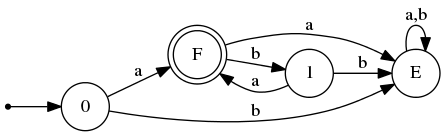
\includegraphics[scale=0.75]{automata1.png}
\end{center}
\end{example}


\begin{defn}[Gramáticas independientes del contexto]
Son aquellas cuyas reglas tienen un único símbolo no terminal en el lado izquierdo.
\end{defn}


\begin{example}[Gramática dependiente de contexto]
\begin{itemize}
\item aSb $\rightarrow$ abb
\item cSd $\rightarrow$ cdd
\end{itemize}
S puede derivarse dependiendo de lo que la rodee, es decir, de su contexto.
\end{example}

\begin{example}[Gramática independiente de contexto (regular)]
\begin{itemize}
\item A $\rightarrow$ aA
\item A $\rightarrow$ a
\end{itemize}
A la derecha tenemos únicamente símbolos terminales o bien símbolos terminales acompañados de un único símbolo no terminal.
Si el elemento no terminal está a la izquierda se denomina gramática lineal por la izquierda. En caso contrario, gramática lineal por la derecha.
\end{example}

\newpage
{\bf Nota a lo anterior:} Una gramática es {\em lineal por la derecha} (right-linear) si todas sus reglas de producción son de una de las dos formas siguientes:

\begin{itemize}
\item B $\rightarrow$ aA
\item B $\rightarrow$ a
\end{itemize}

\noindent con $A, B \in N$ y $a \in T^{*}$. Una gramática es {\em lineal por la izquierda} (left-linear) si todas sus reglas de producción son de una de las dos formas siguientes:

\begin{itemize}
\item B $\rightarrow$ Aa
\item B $\rightarrow$ a
\end{itemize}

\noindent con $A, B \in N$ y $a \in T^{*}$. Una gramática es {\em regular} si es lineal por la izquierda o lineal por la derecha. Todas las gramáticas regulares son independientes del contexto.

\begin{defn}[Equivalencia de gramáticas]
Dos gramáticas son equivalentes si generan el mismo lenguaje
\end{defn}

\section{Gramáticas independientes del contexto}
Como ya vimos una gramática puede representarse como una cuádrupla G=(N,T,S,P), es decir, consta de símbolos no terminales, símbolos terminales, un axioma y unas reglas de producción.

En el caso de una gramática independiente del contexto las reglas de P son de la forma:
\begin{itemize}
\item $A \rightarrow x$

Con $A\in N$, $x \in \Sigma^*$ con $\Sigma=T\cup N$
\end{itemize}

\begin{example}
El lenguaje:
\[L = \lbrace ww^R : w \in (a+b)^*\rbrace\]
es independiente del contexto puesto que puede representarse por medio de una gramática G independiente del contexto, que sería:
\begin{itemize}
\item $S \rightarrow aSa$
\item $S \rightarrow bSb$
\item $S \rightarrow \lambda$
\end{itemize}

\newpage
Para demostrar que el lenguaje generado por la gramática, L(G), es el mismo que L, habría que hacer dos cosas:

\begin{enumerate}
\item Probar que cualquier palabra de $L(G)$ está en $L$.
\item Probar que cualquier palabra de $L$ está en $L(G)$.
\end{enumerate}

El punto 1 es fácil de ver, pues está claro que cualquier cadena generada por $G$ es simétrica (siempre que añadimos una $a$ al principio añadimos otra al final, y lo mismo para $b$).

Para demostrar el punto 2 vamos a probar que si $w \in L$ entonces $w \in L(G)$ usando inducción:

\begin{itemize}
\item Todas las cadenas de $L$ tienen un número par de símbolos: $|w| = 2n$  $\forall w \in L$, $n=0,1,2,...$

\item Para $n=0$ tenemos $w = \lambda \in L$ y se cumple que $w \in L(G)$. Tomamos este caso como base de la inducción.

\item Supongamos que se cumple la hipótesis para $n$: si $w \in L$ con $|w| = 2n$ entonces $w \in L(G)$.

\item Demostremos que se cumple la hipótesis para $n+1$:

Sea $w \in L$ con $|w| = 2n+2$. Entonces $w$ debe ser de la forma $ava$ o $bvb$ con $v \in L$ y $|v| = 2n$. Por hipótesis tenemos que $v \in L(G)$, es decir se puede generar a partir del axioma $S$. Finalmente si $w = ava$ podemos generarla a partir del axioma con la regla $S \rightarrow aSa$, y si $w = bvb$ podemos generarla a partir del axioma con la regla $S \rightarrow bSb$. Por tanto también $w \in L(G)$.

\end{itemize}

\end{example}

\begin{defn}[Derivación directa]
Dada una gramática independiente del contexto G=(N,T,S,P) y sean $v$, $w$ dos formas sentenciales, decimos que w es derivación directa de v:
\[v \rightarrow w\ \equiv v=xZy \wedge w=x\alpha y \wedge \exists \ regla \ en \ P \tq Z \rightarrow \alpha\]
\end{defn}

\noindent con $Z \in N$ y $\alpha \in \Sigma^{*}$.

\begin{defn}[Derivación]
Dada una gramática G=(N,T,S,P) y sean $v$, $w$ dos formas sentenciales, decimos que w es derivación de v, y lo escribimos $v \rightarrow^{+} w$, si existe una cadena de formas sentenciales $a_{0}$, $a_{1}$, $a_{2}$,... $a_{n}$, tales que:
\[v = a_0 \rightarrow a_1 \rightarrow a_2 \rightarrow ... \rightarrow a_n = w\]
\end{defn}

\newpage
\begin{defn}[Lenguaje generado por G]
Dada una gramática G=(N,T,S,P) definimos el lenguaje generado por ella como:
\[L(G) = \lbrace w \in T^*: S \rightarrow^{+} w \rbrace\]
\end{defn}


Veamos algunos ejemplos:

\begin{example}
Dado el lenguaje:
\[L = \lbrace a^n b^n : n\geq 0 \rbrace\]

La gramática que genera este lenguaje es:
\begin{itemize}
\item $S \rightarrow \lambda$
\item $S \rightarrow aSb$
\end{itemize}
\end{example}

\begin{example}
Dado el lenguaje:
\[L = \lbrace w \in (a+b)^* \tq n_a(w)=n_b(w)\rbrace\]

La gramática que genera este lenguaje es:
\begin{itemize}
\item $S \rightarrow aSb | bSa | \lambda$
\item $S \rightarrow SS$
\end{itemize}

Para construirla nos hemos fijado en que una palabra w puede ser de 4 formas:
\[w = \left\{ \begin{array}{lcc}
             aw_0b &   con  & w_0 \in L \\
             \\ bw_0a &  con & w_0 \in L \\
             \\ aw_0a  \Rightarrow  w = w_1w_2  & con  & w_1,w_2 \in L\\
             \\ bw_0b  \Rightarrow  w = w_1w_2  &  con &  w_1,w_2 \in L
             \end{array}
   \right.\]
\end{example}

Una sentencia puede ser derivada de diferentes formas a partir de una misma gramática. Para estos casos vamos a definir derivaciones ``leftmost'' y ``rightmost'':

\begin{defn}[Leftmost]
Consiste en derivar, en cada paso, el elemento no terminal colocado más a la izquierda. Se deja para el lector el arduo trabajo de deducir que significa una derivación ``rightmost''.
\end{defn}

Esto nos lleva a definir un nuevo concepto:

\begin{defn}[Ambigüedad]
Una gramática se define como ambigua si existen dos o más \textbf{árboles de derivación distintos} para la misma sentencia.

Otra forma de definirlo sería considerar ambiguas aquellas gramáticas para las que existen dos \textbf{derivaciones leftmost (o rightmost)} distintas para la misma sentencia.
\end{defn}

\begin{example}
Consideremos la gramática dada por las reglas:
\begin{itemize}
\item $E \rightarrow E + E | E \times E | I$
\item $I \rightarrow a | b | c$
\end{itemize}

Se trata de una gramática ambigua ya que la sentencia $a+b\times c$ tiene dos derivaciones distintas leftmost.
\begin{enumerate}
\item $E \rightarrow E + E \rightarrow I + E \rightarrow a + E \rightarrow a + E \times E \rightarrow a + I \times E \rightarrow a + b \times E \rightarrow a + b \times I \rightarrow a + b \times c$
\item $E \rightarrow E \times E \rightarrow E + E \times E \rightarrow I + E \times E \rightarrow a + E \times E \rightarrow a + I \times E \rightarrow a+b \times E \rightarrow a + b \times I \rightarrow a + b \times c$
\end{enumerate}
\end{example}

Ya vimos que dos gramáticas son equivalentes si generan el mismo lenguaje pero vamos a recalcar que hay \textbf{infinitas} gramáticas que generan el mismo lenguaje.

Dada una gramática G=(T,N,S P) para obtener otra equivalente basta con hacer otra:
\[G' =(T, N \cup \lbrace Z \rbrace, Z, P \cup \lbrace Z \rightarrow E \rbrace)\]

\newpage

\chapter{Autómatas finitos: deterministas y no deterministas}
\begin{defn}[Autómata finito determinista]
Se representa como:
\[ A=(Q, \Sigma, \delta, q_0, F)\]
 donde:
\begin{itemize}
\item Q = conjunto de estados
\item $\Sigma$ =  alfabeto de entrada
\item $\delta$ = función de transición: $\delta : Q\times \Sigma \rightarrow Q$
\item $q_0$ = estado inicial $\in$ Q
\item F = conjunto de estados finales, $F \subset Q$
\end{itemize}
\end{defn}

% La función de transición no es inyectiva, dos elementos del dominio pueden tener la misma imagen (desde dos estados distintos se puede pasar al mismo estado).
%\begin{defn}[Autómata Finito Determinista. AFD\IS]
%Implica que la función de transición es inyectiva. Dado un estado y una entrada sólo hay un estado al que podamos pasar.
%\[\delta: Q \times \Sigma \rightarrow Q\]
%\end{defn}

\begin{defn}[Función de transición extendida\IS]
Consiste en una extensión de la función de transición a cadenas. Se representa como $\delta ^*$:
\[\delta^*(q, w)=q_1\]
Siendo $w\in \Sigma ^*$, $q$ el estado en el que comenzamos y $q_1$ el estado al que llegamos tras procesar toda la palabra. Recordemos que $\Sigma$ es el alfabeto de entrada (conjunto de símbolos) y $\Sigma^*$ es el conjunto formado por todas las posibles cadenas de símbolos que puedes crear con dicho alfabeto.
\end{defn}

\begin{defn}[Lenguaje aceptado\IS por un AFD]
El lenguaje aceptado por un autómata finito determinista, A, es el conjunto de palabras que llevan al autómata a un estado final.
\[L(A) = \lbrace w \in \Sigma^* \ : \ \delta^*(q_0, w) \in F \rbrace\]
\end{defn}

Veamos algún ejemplo:
\begin{example}
Queremos un autómata que reconozca el lenguaje: L=$\lbrace$101,110$\rbrace$

El autómata resultado es:
\begin{center}
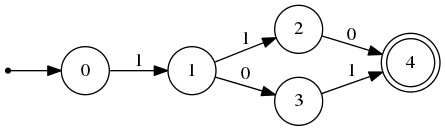
\includegraphics[scale=0.75]{automata2.png}
\end{center}
\obs: Un autómata determinista tiene que tener todas las transiciones definidas, se sobreentiende que las transiciones que no están dibujadas van a un sexto estado en el cual se quedan colgadas.

Este autómata es determinista y su transición de estados dada una entrada "101" sería:

 \begin{tabbing}
   \hspace*{2cm} \= \hspace*{2cm} \= \hspace*{2cm} \= \hspace*{2cm} \= \kill
  entrada:\> 1   \> 0   \> 1   \\
 q0 \> q1 \> q3 \> q4  \\
 \end{tabbing}

Por tanto "101" forma parte del lenguaje del autómata.

Pero podríamos representar el mismo lenguaje con un autómata no determinista:
\begin{center}
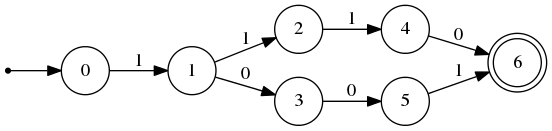
\includegraphics[scale=0.75]{automata3.png}
\end{center}
Y su transición de estados dada una entrada "101" sería:

 \begin{tabbing}
   \hspace*{2cm} \= \hspace*{2cm} \= \hspace*{2cm} \= \hspace*{2cm} \= \kill
  entrada: \> 1   \> 0   \> 1  \\
 q0 \> q1 \> q4 \> q5\\
  \> q2 \> - \> - \\

 \end{tabbing}

Como al menos uno de los caminos lleva a un estado final, la cadena "101" forma parte del lenguaje del autómata (los guiones indican transición no definida, o a un estado vacío).

La ventaja de un autómata no determinista es que podemos explorar varias ramas en paralelo.
\end{example}


\begin{defn}[Transición $\lambda$]
Transición que puede ocurrir sin consumir ningún valor de entrada. Un autómata finito que tenga transiciones de este tipo se considera no determinista.
\end{defn}

\begin{defn}[Autómata finito no determinista. AFN\IS]
Autómata con función de transición de la forma:
\[\delta: Q\times (\Sigma \cup \lbrace \lambda \rbrace) \rightarrow 2^Q\]
Es decir, dado un estado y una entrada (posiblemente vacía) salta a un conjunto de estados.
\end{defn}

\begin{defn}[Función de transición de un AFN extendida\IS]
Consiste en una extensión de la función de transición a cadenas. Se representa como $\delta ^*$:
\[\delta^*(q, w) = E\]
Siendo $w\in \Sigma ^*$, $q$ el estado en el que empezamos y $E$ el conjunto de estados a los que llegamos tras procesar toda la palabra.
\end{defn}

\begin{defn}[Lenguaje aceptado\IS por un AFN]
El lenguaje aceptado por un autómata finito no determinista, A, es el conjunto de palabras que llevan al autómata a un estado final.
\[L(A) = \lbrace w \in \Sigma^* \ : \ \delta^*(q_0, w)\cap F \neq \emptyset \rbrace\]
\end{defn}

\begin{example}
Diseñar un autómata para el siguiente lenguaje

Tenemos el alfabeto: $\Sigma = \lbrace 0,1,2,3,4,5,6,7,8,9,+,-,\cdot \rbrace$ con las siguientes restricciones:
\begin{enumerate}
\item Signo puede o no aparecer
\item Parte decimal puede aparecer o no
\item Parte entera puede o no aparecer
\item Debe haber al menos parte entera o decimal.
\end{enumerate}

El autómata queda:
\begin{center}
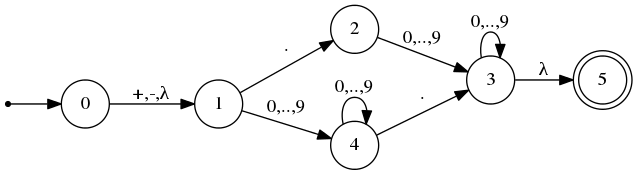
\includegraphics[scale=0.75]{automata4.png}
\end{center}
\end{example}

\newpage

\begin{defn}[Fuentes de indeterminismo de un AF]
Un autómata finito no determinista se caracteriza por tener alguna de las siguientes propiedades:
\begin{enumerate}
\item Con la misma entrada, varias transiciones posibles para un mismo estado.
\item Hay transiciones lambda
\item Se puede transitar a $\emptyset$ (transiciones no definidas)
\end{enumerate}
\end{defn}

\begin{example}
Otro ejemplo de autómata no determinista podría ser:
\begin{center}
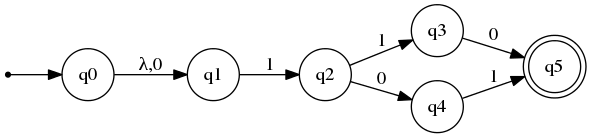
\includegraphics[scale=0.75]{automata3a.png}
\end{center}
Cuya transición de estados dada una entrada "101" sería:

 \begin{tabbing}
   \hspace*{2cm} \= \hspace*{2cm} \= \hspace*{2cm} \= \hspace*{2cm} \= \hspace*{2cm} \kill
 Estados \> 1   \> 0   \> 1   \\
 q0 \> - \> - \> -  \\
 q1 \> q2 \> q4 \> q5\\
 \end{tabbing}

En este autómata, podemos avanzar al estado 'q1'  a través de la transición $\lambda$, aunque el primer símbolo de la entrada sea un '1', (segunda línea de la tabla). Sin embargo en el camino en el que nos mantenemos en el estado 'q0'  (primera línea de la tabla), no tenemos la transición definida con entrada '1' y vamos al estado vacío. Llegamos a un estado final, por tanto la palabra "101" pertenece al lenguaje de este autómata.

\end{example}

\begin{theorem}
Los autómatas finitos no deterministas y deterministas son equivalentes.
\end{theorem}

Esto significa que dado un autómata finito determinista que acepta un determinado lenguaje, existe otro no determinista que acepta el mismo lenguaje, y viceversa. Se utilizan los AFN por comodidad, porque las demostraciones formales son más sencillas.

\section{Equivalencia entre AF y ER}
Vamos a ver cuál es la relación existente entre los autómatas finitos y las expresiones regulares.

Como ya vimos una gramática puede expresarse como una cuádrupla G=(N,T,S,R), es decir, consta de símbolos no terminales, símbolos terminales, un símbolo inicial o axioma y unas reglas de producción.

Recordamos también que una gramática regular es aquella que es lineal por la derecha o lineal por la izquierda

Hay 4 formas de representar un lenguaje regular, y en ellas reside la equivalencia entre autómatas finitos y expresiones regulares. Las 4 formas de representar un lenguaje regular son:
\begin{enumerate}
\item Describiendo todos sus componentes
\item Con una gramática regular
\item Con una expresión regular
\item Mediante un AFN/AFD
\end{enumerate}

\newpage


%%%%%%%%%%%%%%%%%%%%%%%%%%%%%%%%%%%%%%%%%%%%%%%%%%%%%%%%%%%%%%%%%%%%%%%%


\chapter{Autómatas a pila}
Dado el lenguaje:
\[L=\lbrace ww^R \tq w \in (0+1)^*\rbrace\]
que representa palabras capicúas sobre $\lbrace 0, 1\rbrace$ con un número par de símbolos, vamos a intentar construir un autómata finito para él.

Esto no es posible ya que siempre necesito llegar hasta la mitad de la palabra ``almacenando'' lo que hemos leído para después comprobar que lo leemos al revés. Puesto que la palabra puede tener longitud arbitraria, necesitaremos una cantidad de memoria arbitraria y esto no es viable (sería necesario un autómata con un número infinito de estados).

Es aquí donde surgen los autómatas a pila. Estos autómatas se caracterizan por que en cada salto indicamos una entrada, saca el símbolo de la cima de la pila y añade una cadena a la pila.

Para el lenguaje dado, el autómata a pila que lo representa sería:

\begin{center}
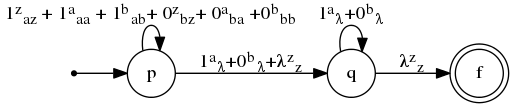
\includegraphics[scale=0.75]{automata5.png}
\end{center}
En teoría, las etiquetas de los arcos del autómata son de la forma:
\[A_b^c\]
donde $A$ sería la entrada leída, $b$ el elemento que extraemos del tope de la pila y $c$ la cadena que insertamos en la pila. Por tanto una transición solo se puede dar si aparte de tener la entrada correspondiente, la cima de la pila coincide con lo que vamos a extraer de ella. Introducir $az$ implica que la 'a' se queda como cima de la pila, y la 'z' detrás.

En algunos ejercicios usaremos la notación $\{b,A,c\}$ con idéntico significado.

\newpage
\begin{defn}[Autómata a pila]
Un autómata a pila se representa como:
\[A=(Q, \Sigma, \delta, q_0, F, \topl, A_0)\]
siendo:
\begin{itemize}
\item $Q$: conjunto de estados
\item $\Sigma$: alfabeto de entrada
\item $\delta$: función de transición: $\delta:Q\times(\Sigma \cup \{\lambda\})\times \topl \rightarrow 2^{Q\times \topl^*}$
\item $q_0$: estado inicial $\in Q$
\item $F$: conjunto de estados finales
\item $\topl$: alfabeto de la pila
\item $A_0$: símbolo inicial de la pila $\in \tau$
\end{itemize}

\noindent {\bf Nota:} En realidad el codominio de $\delta$ es el conjunto de subconjuntos finitos de $Q\times \topl^*$.

Básicamente consiste en un autómata, como los vistos hasta ahora, acompañado de una pila en la que realizaremos inserciones y extracciones en cada transición.
\end{defn}

Vamos a ver un pequeño ejemplo que explica cómo entender la función de transición:
\begin{example}
La evaluación de la función de transición:
\[\delta(q,a,x)=\{(p,y)\}\]

\noindent con $q, p \in Q$, $a \in \Sigma$, $x \in \topl$ y $y \in \topl^{*}$.
Implica que, estando en el estado 'q', ante una entrada 'a', habiendo en la cima de la pila un 'x' pasamos al estado 'p', insertando en la pila 'y', y sacando la 'x'.
\end{example}

En estos autómatas los conceptos de determinismo o no determinismo se mantienen. Es decir, un autómata a pila será no determinista si dada una entrada y un elemento a extraer de la cima de la pila tiene varias acciones que puede llevar a cabo (varios pares ('estado','inserción en pila')). Profundizaremos más adelante en este concepto.

\obs Aunque un autómata finito determinista es equivalente a uno no determinista, con autómatas a pila no ocurre lo mismo.

\begin{defn}[Autómata a pila determinista]
Un autómata a pila será determinista si cumple las siguientes condiciones:
\begin{itemize}
\item No hay transiciones $\lambda$ o, si las hay, no hay ninguna otra transición con un símbolo diferente. Es decir, si desde un estado p y con a en la pila pudieras pasar a otro q por una transición lambda, no habría otra posible transición desde el estado p y con a en la pila.
\item Dada una situación (estado p, símbolo de entrada x y símbolo a en la cima de la pila) $\delta (p,x,a)$ contiene como mucho un elemento $(q,b)$.
\end{itemize}
\end{defn}

\begin{defn}[Descripción instantánea]
Se trata de una representación de la situación actual del autómata. (q,X,A) es una descripción instantánea donde:\\
\begin{enumerate}
\item q = Nodo/estado en el que nos encontramos
\item X = Entrada que falta por leer, $X \in \Sigma^{*}$
\item A = Contenido de la pila, $A \in \topl^{*}$
\end{enumerate}

Dada una descripción instantánea podemos continuar el procesamiento de la cadena sin perder información.
\end{defn}

\begin{defn}[Precedencia entre descripciones instantáneas]
Decimos que una descripción instantánea precede a otra:
\[(q,xX,aA) \vdash (p, X, bA)\]
si:
\[(p,b) \in \delta(q, x, a)\]
Siendo 'p','q' nodos del autómata, 'x' el siguiente símbolo de entrada que se va a leer, 'X' el resto de la cadena de entrada; 'a' el carácter que hay en la cima de la pila, 'A' el resto del contenido de la pila y,'b' una cadena de símbolos que insertamos en la pila. En este transición se lee 'x', se saca 'a' de la cima de la pila y se introduce 'b'.

Es decir, una descripción instantánea precede a otra si hay una transición que nos lleva de una a otra.

\end{defn}

\begin{defn}[Precedencia *]
Decimos que hay precedencia * entre dos descripciones instantáneas:
\[(q,X,A) \vdash^* (p, Y, B)\]
cuando hay una secuencia $d_0,d_1,..., d_n$ de descripciones instantáneas tales que:
\[(q,X,A) = d_0 \vdash d_1 \vdash ... \vdash d_n = (p, Y, B)\]
\end{defn}

\noindent con $p, q \in Q$, $X, Y \in \Sigma^{*}$ y $A, B \in \topl^{*}$.

Basándonos en estas definiciones, podemos representar el lenguaje aceptado por un autómata a pila como:
\[L(A) = \lbrace w \in \Sigma^* \tq (q_0, w, A_0) \vdash^* (p, \lambda, X)\rbrace\]
con $p\in F, X \in \topl^*$

\begin{example}
Queremos encontrar un autómata que represente el lenguaje:
\[L = \lbrace a^nb^n, n \geq 0\rbrace\]

El autómata de pila que representa este lenguaje es:

\begin{center}
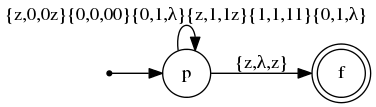
\includegraphics[scale=0.75]{automata6.png}
\end{center}
\end{example}

\newpage
\chapter{Gramáticas de atributos}
Un compilador se encarga de generar el código máquina a partir de un código dado.

En primer lugar debemos saber que un compilador realiza tres tareas:
\begin{enumerate}
\item \textbf{Análisis morfológico}. A estas alturas consideramos que ya nos viene hecho y no nos preocupamos por ello.
\item \textbf{Análisis sintáctico}. Consiste en construir el árbol de derivación. Es decir, se comprueba que la sentencia obtenida sale de derivar el axioma.
\item \textbf{Análisis semántico}. Consiste en recorrer el árbol de derivación calculando atributos y realizando comprobaciones semánticas.
\end{enumerate}

Vamos a centrarnos ahora en análisis semántico.
\section{Análisis semántico}

Vamos a explicar brevemente la idea que hay detrás de esto:

Partiendo de una gramática independiente del contexto, y derivando el axioma hasta obtener una sentencia, queremos obtener alguna función específica de nuestra gramática.

Es entonces cuando surgen las gramáticas de atributos, que añaden lo siguiente a la gramática independiente del contexto:
\begin{itemize}
\item Incorporan atributos a los nodos no terminales.

\item Incorporan funciones sobre esos atributos en las reglas de derivación. (Además veremos que estas funciones se podrán realizar en instantes concretos).

\item Incorporan una \textbf{información global} a la gramática. La información global está formada por un conjunto de variables que son accesibles desde cualquier nodo del árbol.
\end{itemize}
Por tanto, una vez obtenido el árbol de derivación, el análisis semántico recorrerá dicho árbol utilizando el recorrido en  \textbf{profundidad por la izquierda y con vuelta atrás} (lo explicamos más adelante) corroborando el buen funcionamiento de estas nuevas funciones.

El paso de información de un nodo a otro del árbol se podrá realizar mediante tres métodos:

\begin{itemize}
\item Síntesis: la información se propaga del nodo inferior al nodo superior.

\item Herencia: la información se propaga del nodo superior al nodo inferior.

\item Usando la información global.
\end{itemize}

Vamos a ver un ejemplo con detalle, explicando sobre él algunos de los conceptos:

Como hemos dicho, la idea es que dada una gramática independiente del contexto, podemos conseguir que esta realice funciones específicas. Lo conseguimos añadiendo atributos y especificaciones a las reglas de derivación.

\begin{example}
Consideremos la gramática:
\[G=\{\{(,)\}, \{L,I\}, L, P\}\]
Con las reglas de derivación P:
\begin{itemize}
\item $L \rightarrow (I)$
\item $I \rightarrow (I)$
\item $I \rightarrow II$
\item $I \rightarrow λ$
\end{itemize}

En primer lugar vamos a derivar el axioma y obtener una sentencia, nos queda (por ejemplo) el siguiente árbol de derivación:

\begin{forest}
for tree={
  draw,
  minimum height=1cm,
  anchor=north,
  align=center,
  child anchor=north
},
[{L}, align=center, name=SS
  [$($, tier=word]
  [{I}, name=PDC
    [{I}, name=MS
      [{$($}, tier=word]
      [{I}
        [{λ}, tier=word]]
      [{$)$}, tier=word]]
    [{I}
      [{$($}, tier=word]
      [{I}
        [{$($}, tier=word]
        [{I}
          [{λ}, tier=word]]
        [{$)$}, tier=word]]
      [{$)$}, tier=word]]
    ]
    [{$)$}, tier=word]
 ]
\end{forest}

Vemos que sintácticamente es correcto ya que se obtiene de derivar el axioma $L$.

Queremos hacer que esta gramática nos devuelva la profundidad de una expresión, es decir, el máximo número de paréntesis contenidos unos en otros.

Para ello, vamos a utilizar gramática de atributos, en primer lugar debemos añadir a los elementos L e I un atributo profundidad.

Vamos a intentar hacerlo propagando el atributo profundidad hacia arriba (es decir, usando síntesis). Por ello, un nodo terminal como sería λ debería tener profundidad 0. Por lo que la cuarta regla queda de la forma:
\[I \rightarrow λ \{I.prof=0\}\]

En las dos primeras reglas, debemos realizar una propagación hacia arriba, aumentando en uno la profundidad. Así estas dos primeras reglas quedan de la forma:
\[L \rightarrow (I) \{L.prof = I.prof+1\}\]
\[I_1 \rightarrow (I_2) \{I_1.prof=I_2.prof+1\}\]

Para la tercera regla, podemos ver que la profundidad que asciende será el máximo de las profundidades de cada uno de los símbolos en los que deriva. La tercera regla quedaría:
\[I_1 \rightarrow I_2I_3 \{I_1.prof = max(I_2.prof, I_3.prof)\}\]

Si ahora analizamos los instantes en que se realizaría la función de cada regla y agrupamos todo lo indicado anteriormente llegamos a:
\[G=\{\{(,)\}, \{L(prof),I(prof)\}, L, P, \emptyset \}\]
Con P:
\begin{itemize}
\item $L \rightarrow (I) \{2: \ L.prof = I.prof+1\}$
\item $I_1 \rightarrow (I_2) \{2: \ I_1.prof=I_2.prof+1\}$
\item $I_1 \rightarrow I_2I_3 \{2: \ I_1.prof = max(I_2.prof, I_3.prof)\}$
\item $I \rightarrow λ \{0: \ I.prof=0\}$
\end{itemize}

Así, hemos conseguido una gramática de atributos que realiza una función específica (obtener la profundidad). Lo hemos logrado a partir de una gramática independiente del contexto añadiendo atributos y el instante en el que debo realizar cada asignación en las reglas de derivación.

Además, una gramática de atributos contiene una información global. En este caso no la vamos a usar por lo que la declaramos vacía (es el último símbolo que se ha añadido a G).

También debemos saber que el árbol se recorre en \textbf{profundidad por la izquierda y con vuelta atrás}. Esta técnica consiste en recorrer siempre el hijo más a la izquierda, cuando no queden hijos a la izquierda, continuamos con el siguiente hijo más a la izquierda. Cuando no queden hijos volvemos al nodo superior y así sucesivamente.

Si suponemos un caso simple en el que un nodo raíz tiene n hijos inmediatos, podemos ver que al aplicar este procedimiento recorremos el nodo raíz n+1 veces. Por tanto el nodo raíz tendrá n+1 instantes.

Vamos a dejar claro a qué nos referimos con el instante en el que realizo la función de cada regla. Para ello, debemos saber que al realizar el análisis semántico cada nodo sabe qué regla de derivación se ha usado sobre él, y por tanto conocerá el número de hijos inmediatos que tiene. Así, por ejemplo un nodo I al que le aplicamos la regla $I_1 \rightarrow I_2 I_3$, tiene 3 instantes:

-El instante 0, en el que se visita el nodo $I_1$.

-El instante 1, en el que se vuelve al nodo $I_1$ después de haber visitado el nodo $I_2$.

-El instante 2, en el que se vuelve al nodo $I_1$ después de haber visitado el nodo $I_3$.

Veamos ahora como queda el árbol realizando el recorrido en profundidad por la izquierda y con vuelta atrás y aplicando las distintas funciones:

\begin{forest}
for tree={
  draw,
  minimum height=1cm,
  anchor=north,
  align=center,
  child anchor=north
},
[{L\\0:nada\\ p=2 en instante 2}, align=center, name=SS
  [$($, tier=word]
  [{$I^1$\\p=2 en instante 2}, name=PDC
    [{$I^2$\\p=1 en instante 2}, name=MS
      [{$($}, tier=word]
      [{$I^4$\\p=0 en instante 0}
        [{λ}, tier=word]]
      [{$)$}, tier=word]]
    [{$I^3$\\p=2 en instante 2}
      [{$($}, tier=word]
      [{$I^5$\\p=1 en instante 2}
        [{$($}, tier=word]
        [{$I^6$\\p=0 en instante 0}
          [{λ}, tier=word]]
        [{$)$}, tier=word]]
      [{$)$}, tier=word]]
    ]
    [{$)$}, tier=word]
 ]
\end{forest}

Hemos puesto superíndices a las I para poder referirnos ahora a ellas:

El recorrido en profundidad de esté árbol quedaría:

Empezamos en L, estamos en el instante 0 de L... bajamos a $($, como es terminal no hacemos nada... subimos a L, instante 1 de L... bajamos a $I^1$, instante 0 de $I^1$...bajamos a $I^2$, instante 0 de $I^2$... bajamos a $($ como es terminal no hacemos nada... subimos a $I^2$, instante 1 de $I^2$...bajamos a $I^4$, instante 0 de $I^4$, que como es un nodo que deriva con la regla $I\rightarrow \lambda$ le aplicamos la función $I.prof=0$... subimos a $I^2$, instante 2 de $I^2$, que como es un nodo que deriva con la regla $I_1\rightarrow (I_2)$, le aplicamos la función $I_1.prof=I_2.prof+1$, por tanto tenemos ahora mismo $I^2.prof=1$... bajamos a $)$, como es un nodo terminal no hacemos nada... subimos a $I^2$, instante 3 de $I^2$... subimos a $I^1$, instante 1 de $I^1$... bajamos a $I^3$, instante 0 de $I^3$... etc etc etc.

\end{example}



\begin{example}
Vamos a apoyarnos en la gramática definida en el ejemplo anterior y a modificar simplemente las acciones, con el fin de obtener un programa que cuente el número de listas (parejas de paréntesis).

Vamos a realizarlo de tres formas distintas: con síntesis, herencia y con información global. Estas diferentes formas dan lugar a diferentes acciones, pero el árbol de derivación sigue siendo el mismo.

Cada una de las reglas de derivación serían:

\begin{itemize}
\item \textbf{Síntesis}
\[G=\{\{(,)\}, \{L(n),I(n)\}, L, P\}\]
\begin{itemize}
\item $L \rightarrow (I) \{2: \ L.n = I.n+1\}$
\item $I_1 \rightarrow (I_2) \{2: \ I_1.n=I_2.n+1\}$
\item $I_1 \rightarrow I_2I_3 \{2: \ I_1.n = I_2.n + I_3.n)\}$
\item $I \rightarrow λ \{0: \ I.n=0\}$
\end{itemize}

\item \textbf{Herencia}
\[G=\{\{(,)\}, \{L(n),I(antes, despues)\}, L, P\}\]
\begin{itemize}
\item $L \rightarrow (I) \{0: \ I.antes=1, \ 2: \ L.n=I.despues\}$
\item $I_1 \rightarrow (I_2) \{0: I_2.antes = I_1.antes+1, \ 2: \ I_1.despues=I_2.despues\}$
\item $I_1 \rightarrow I_2I_3 \{0: \ I_2.antes = I_1.antes, \ 1: \ I_3.antes=I_2.despues, \ 2: \ I_1.despues=I_3.despues\}$
\item $I \rightarrow λ \{0: \ I.despues=I.antes\}$
\end{itemize}
Hemos usado alguna acción que se sale de un esquema puro de herencia por ser imposible realizarlo de otra forma.

\item \textbf{Información global}
\[G=\{\{(,)\}, \{L,I\}, L, P, \{n\}\}\]
\begin{itemize}
\item $L \rightarrow (I) \{0: \ n=0; \ 1: \ n = n+1\}$
\item $I_1 \rightarrow (I_2) \{0: \ n=n+1\}$
\item $I_1 \rightarrow I_2I_3$
\item $I \rightarrow λ $
\end{itemize}
Este caso es bastante más sencillo, pues en cada derivación tienes acceso al contador global y basta con incrementarlo, sin preocuparte por los sucesores.

Usando información global es realmente importante \textbf{indicar los instantes en que se realiza cada acción} puesto que de lo contrario habría lugar a confusión. (En los casos anteriores los atributos imponían un orden sin ambigüedad).

\end{itemize}
\end{example}

En las transparencias podéis ver estos tres ejemplos para diferenciar la herencia, la síntesis y la información global (llamada tabla de símbolos):

\includepdf[frame=true, noautoscale=true, delta=10 10, nup=2x4,pages={2-9}, scale=0.72]{pdf/GramaticaAtributos.pdf}

\includepdf[frame=true, noautoscale=true, delta=10 10, nup=2x4,pages={10-17}, scale=0.72]{pdf/GramaticaAtributos.pdf}

\includepdf[frame=true, noautoscale=true, delta=10 10, nup=2x4,pages={18-25}, scale=0.72]{pdf/GramaticaAtributos.pdf}

\includepdf[frame=true, noautoscale=true, delta=10 10, nup=2x4,pages={26-27}, scale=0.72]{pdf/GramaticaAtributos.pdf}

\begin{example}
Para ver claramente las diferencia entre análisis semántico y sintáctico nos podemos fijar en lo siguiente, según el ejemplo 1, el código:
\begin{verbatim}
                           int _x,_y
                               _x=7
\end{verbatim}
es correcto semántica y sintácticamente, mientras que el código:
\begin{verbatim}
                           int _x,_y
                               _z=7
\end{verbatim}
es sintácticamente correcto pero no semánticamente.
\end{example}

\begin{example}
Vamos a tomar un caso sencillo con dos reglas sacadas del último ejemplo mostrado en las transparencias. La semántica es:
\begin{itemize}
\item $L \rightarrow i \{st(i.nombre,L.tipo\}$
\item $A \rightarrow i = E \{in TS (i.nombre)==true; \; gt(i.nombre)==E.tipo; \; sv(i.nombre, E.valor)\} $
\end{itemize}

Para la primera regla, el orden en que se recorrería el árbol de derivación es:
\begin{verbatim}
- En el instante 0 bajamos del nodo L al nodo i,
- En el instante 1 volvemos al nodo L.
\end{verbatim}

Como es lógico, la operación de setType representada en la gramática no puede realizarse hasta conocer el tipo de L y el nombre de i, por lo que se realiza en el instante 1.

Lo representaríamos como:
\[L \rightarrow i \{1:st(i.nombre,L.tipo\}\]

Vamos ahora con la segunda regla. El orden en el que se recorrería el árbol de derivación seria:
\begin{verbatim}
- En el instante 0 bajamos del nodo A al nodo i, en el instante 1 volvemos al A.
- En ese instante bajaríamos al nodo =, del que volveríamos en el instante 2.
- Por último bajaríamos al nodo E y volveríamos del mismo en el instante 3
\end{verbatim}

Siguiendo esta secuencia y analizando en qué momento tenemos disponibles los valores para cada operación la segunda regla de la gramática sería de la forma:
\[A \rightarrow i = E \{ 1: \ in TS (i.nombre)==true; 3: \ gt(i.nombre)==E.tipo; 3: \ sv(i.nombre, E.valor)\}\]

En este tercer ejemplo es importante añadir algunas comprobaciones más en las reglas, que no vienen en las trasparencias:
\begin{itemize}
\item En la regla $A \rightarrow i=E$ comprobar $inTS(i.nombre)==true$ (es decir, ¿está en la tabla de símbolos i.nombre?)

\item En la regla $E_1 \rightarrow E_2 + E_3$ y $E_1 \rightarrow E_2 * E_3$ comprobar que $E_2.tipo=E_3.tipo$

\item En la regla $E \rightarrow i$ comprobar $inTS(i.nombre)==true$ y $gt(i.nombre)==E.tipo$ con gt=getType (es decir, ¿es el parametro tipo de i.nombre igual al de E?).
\end{itemize}
\end{example}



\chapter{Analizador morfológico}
Empezamos este capítulo recordando la función de un compilador.

Dado un archivo \textit{fuente}, este archivo pasará a través de un analizador de código, que realiza tres funciones, utilizando para ello una tabla de símbolos que él mismo genera:
\begin{itemize}
\item Análisis morfológico
\item Análisis sintáctico
\item Análisis semántico
\end{itemize}
Tras ser analizado, se genera un árbol de derivación como los vistos hasta ahora.

Nos centramos ahora en el analizador morfológico (también llamado léxico o scanner). Este realiza principalmente la siguiente función:

\textbf{Obtención de unidades sintácticas.} Son los llamados tokens. Estos pueden ser identificadores, constantes, palabras reservadas ($if$, $them$, $for$,...) u otros símbolos (simples: $+$, $=$,... o dobles: $:=$,...).\\

No obstante, el analizador morfológico también es importante en la consecución de las siguientes tareas secundarias:
\begin{enumerate}
\item Eliminar delimitadores (espacios en blanco, tabuladores, saltos de línea...).
\item Eliminación de comentarios en el código.
\item Detecta errores morfológicos. (Símbolos inválidos, constantes e identificadores mal construidos...)
\item Inicializa algunas tareas semánticas, es decir, calcula el valor de algunos atributos de constantes o identificadores.
\end{enumerate}

Lo vemos con un ejemplo: tenemos un lenguaje que admite el siguiente tipo de objetos:
\begin{itemize}
\item Identificadores: letra seguida de cero o más dígitos y letras.
\item Constantes: (números enteros).
\item Palabras reservadas: \textit{begin}, \textit{end}, \textit{int}, \textit{print}.
\item Símbolos: tanto simples: ';' como dobles: ':='.
\end{itemize}

Con este lenguaje, y dado el siguiente fichero de entrada  \textit{fuente}.

\begin{verbatim}
    begin
        int A;
        A := 100;
        print A;
    end
\end{verbatim}

El analizador morfológico generará un fichero de salida semejante al siguiente:

\begin{verbatim}
    <"begin",TOK_BEGIN>
    <"int",TOK_INT>
    <"A",TOK_ID, valor='A'>
    .
    .
    .
    <"100",TOK_CONST, valor=100>
    .
    .
    .
\end{verbatim}

La 4ª tarea secundaria, que tenía el analizador morfológico, es la que realiza la función de crear un atributo valor e inicializarlo.

\chapter{Analizador sintáctico}

\section{Introducción}

Para llevar a cabo el análisis sintáctico de una entrada se emplean tablas de análisis. Estas permiten analizar una sentencia, con el fin de saber si se trata de una sentencia válida para una gramática dada o no.

Existen dos tipos de análisis: \textbf{ascendente} y \textbf{descendente}

Veamos un ejemplo:
\begin{example}
Dada la gramática:
\begin{itemize}
\item 1) E $\rightarrow$ E + E
\item 2) E $\rightarrow$ E x E
\item 3) E $\rightarrow$ -E
\item 4) E $\rightarrow$ (E)
\item 5) E $\rightarrow$ id
\end{itemize}

Vamos a realizar un \textbf{análisis ascendente} partiendo de la siguiente sentencia:
\begin{center}
(id+id)xid
\end{center}

Para ello vamos a contar con la ayuda de una pila y nos basaremos en dos reglas básicas:
\begin{enumerate}
\item \textbf{Reducción}
Se aplicará siempre que sea posible. No hay elección.

Se lleva a cabo cuando los elementos de la cima de la pila coinciden con la parte derecha de alguna regla de nuestra gramática.

En este caso se extraen los elementos de la pila y se sustituyen por la parte izquierda de la regla indicada anteriormente.

\item \textbf{Desplazamiento}
Se aplica cuando no puede realizarse ninguna reducción.

Consiste en introducir en la cima de la pila el siguiente elemento de la sentencia que estamos analizando
\end{enumerate}

Aplicando estas reglas a nuestra sentencia obtenemos el siguiente resultado:
\begin{center}
\begin{tabular}{| c | c | c | c |}
\hline
Instante & Entrada & Pila & Acción \\
\hline
0 & (id+id)xid & - & Desplazamiento \\
\hline
1 & id+id)xid & ( & Desplazamiento \\
\hline
2 & +id)xid & (id & Reducción(5) \\
\hline
3 & +id)xid & (E & Desplazamiento \\
\hline
4 & id)xid & (E+ & Desplazamiento \\
\hline
5 & )xid & (E+id & Reducción(5)\\
\hline
6 & )xid & (E+E & Reducción(1) \\
\hline
7 & )xid & (E & Desplazamiento \\
\hline
8 & xid & (E) & Reducción(4) \\
\hline
9 & xid & E & Desplazamiento \\
\hline
10 & id & Ex & Desplazamiento \\
\hline
11 & - & Exid & Reducción(5) \\
\hline
12 & - & ExE & Reducción(2) \\
\hline
13 & - & E & Fin \\
\hline
\end{tabular}
\end{center}
Puesto que en la pila sólo queda el axioma, concluimos que la sentencia es válida para este lenguaje.
\end{example}

Tras este ejemplo podemos definir formalmente el algoritmo de análisis ascendente.

\begin{defn}[Análisis ascendente]
Este algoritmo consiste de dos pasos:
\begin{verbatim}
     Mientras queden elementos en la entrada:
       desplazamos
       mientras podemos reducir:
           reducimos

     Si en la pila sólo está el axioma:
         OK.
     En caso contrario:
         ERROR.
\end{verbatim}
\end{defn}

Una vez visto el análisis ascendente el siguiente paso es estudiar el análisis descendente.

\begin{defn}[Análisis descendente]
Algoritmo para determinar si una entrada es válida o no para una gramática dada mediante derivaciones (partiendo del axioma)

Es decir, tomamos el axioma y aplicamos derivaciones sucesivas intentando llegar a la sentencia que queremos analizar.

Si logramos generar la sentencia que estamos analizando, esta será válida. (En caso contrario no)
\end{defn}

Vamos a trabajar con gramáticas sencillas en las que sólo haya una derivación posible en cada paso. En caso de no ser así deberíamos avanzar todo lo posible para después hacer backtracking, comprobando que no dejamos caminos sin explorar.

Veámoslo con un ejemplo:
\begin{example}
Dada la gramática:
\begin{itemize}
\item E $\rightarrow$ TB
\item B $\rightarrow$ +TB | λ
\item T $\rightarrow$ FX
\item X $\rightarrow$ *FX | λ
\item F $\rightarrow$ i | (E)
\end{itemize}
Vamos a usar un \textbf{análisis descendente} para comprobar si es válida la sentencia:
\begin{center}
i*i
\end{center}
Para hacerlo apoyándonos en una pila, como en el ejemplo anterior, los pasos a seguir son los siguientes:

\begin{tabular}{| c | c | c |}
\hline
Instante & Pila & Acción\\
\hline
1 & E & Derivamos\\
\hline
2 & B | T & Derivamos \\
\hline
3 & B | X | F & Derivamos\\
\hline
4 & B | X | i & Extraemos, pues i está en la sentencia dada\\
\hline
5 & B | X & Derivamos \\
\hline
6 & B | X | F | * & Extraemos, pues * está en la sentencia dada \\
\hline
7 & B | X | F & Derivamos \\
\hline
8 & B | X | i & Estraemos, pues i está en la sentencia dada \\
\hline
9 & B | X & Derivación λ\\
\hline
10 & B & Derivación λ \\
\hline
\end{tabular}

Si al finalizar nos queda la pila vacía concluimos que la sentencia estudiada es correcta.
\end{example}


A lo largo de esta sección profundizaremos sobre el análisis ascendente y el análisis descendente.


\section{Tablas de análisis ascendente}

Vamos a estudiar ahora diferentes tablas de análisis (y autómatas asociados) que se utilizan para realizar el análisis ascendente.

\subsection{Tablas LR(0)}

\begin{defn}[Tabla LR(n)]
Tabla empleada para el procesamiento de entrada desde la izquierda (\textbf{L}eft) mediante derivaciones \textbf{R}ight-most con \textbf{n} símbolos de entrada.

\end{defn}

Veamos un ejemplo de como funciona esta tabla de análisis
\begin{example}
Consideremos la gramática G=(T, N, E, P):
\begin{itemize}
\item E $\rightarrow$ T | E+T
\item T $\rightarrow$ i | (E)
\end{itemize}

El primer paso para realizar el análisis LR(O) consiste en añadir un axioma E' y la regla:
\begin{center}
E' $\rightarrow$ E\$
\end{center}

De forma que se obtiene la siguiente \textbf{gramática extendida}:
\begin{itemize}
\item E' $\rightarrow$ E \$
\item E $\rightarrow$ T
\item E $\rightarrow$ E+T
\item T $\rightarrow$ i
\item T $\rightarrow$ (E)
\end{itemize}

Ahora lo que hacemos es añadir un '.' delante del símbolo que estemos analizando en cada paso.

Para realizar el análisis por este método vamos a construir un autómata finito determinista, que procesa una cadena de símbolos, empezando por el estado S0:

\begin{center}
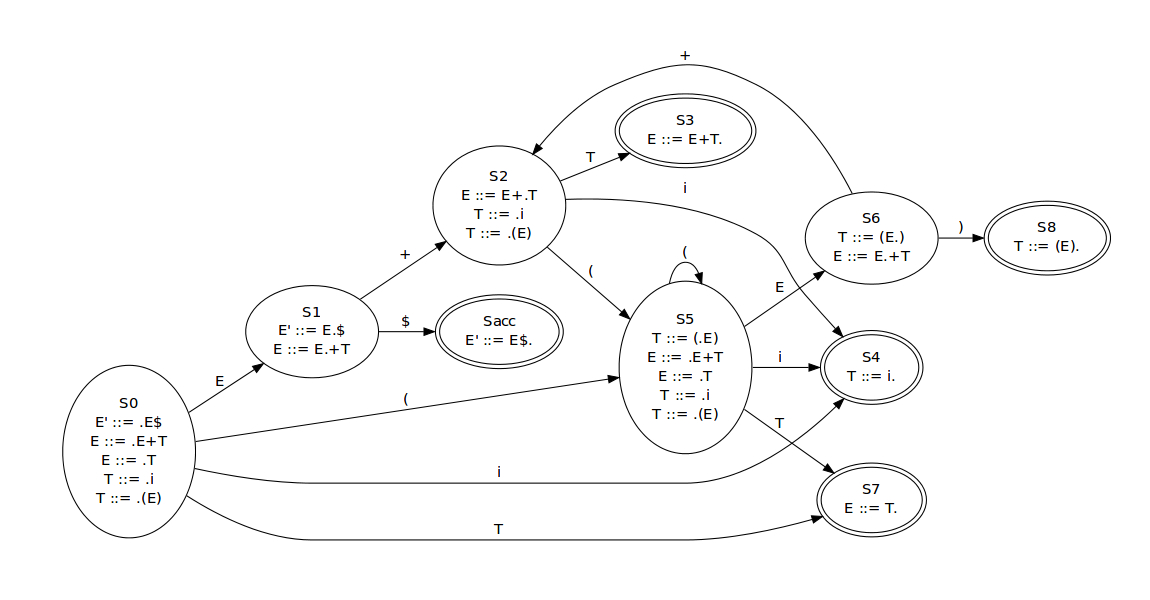
\includegraphics[scale=0.45]{img/automatalr0.jpg}
\end{center}

Si aplicamos el algoritmo de análisis LR(0) a lo bruto, tras cada reducción todo lo que hay en la pila (una vez aplicado el correspondiente cambio fruto de la reducción) pasa al inicio de la cadena de entrada y saltamos al estado $S_0$ para continuar con el análisis.

No obstante, esta práctica implica deshacer lo andado muchas veces y alarga mucho el desarrollo del algoritmo. Para evitar esto, en la pila guardamos, además de la última entrada leída, el estado en que nos encontramos y tras una reducción nos desplazamos al estado indicado en la pila justo antes de la reducción y añadimos la nueva cadena (fruto de la reducción) al inicio de la cadena de entrada.

A continuación explicamos cómo se realiza el análisis a lo bruto.

Si el análisis de una cadena llega al estado de aceptación ($S_{acc}$) en este autómata, se termina el análisis concluyendo que la cadena es sintácticamente correcta.

Para construir el autómata seguimos los siguientes pasos:
\begin{itemize}
\item Partimos en el estado $S_0$ del axioma de la gramática extendida ($E'$).
\item Situamos un '.' delante del símbolo que analizamos, en este caso empezamos por el símbolo E. Ya que la regla de derivación del axioma es $E' \rightarrow E\$$. Por tanto nos queda $E' \rightarrow .E\$$
\item Ahora tenemos que \textbf{cerrar} el símbolo que esta inmediatamente después del punto. Si es un terminal ya estaría cerrado. Si es un no terminal lo cerramos escribiendo las reglas de derivación del mismo, poniendo de nuevo un '.' delante del primer símbolo de cada una de las reglas y cerrando el símbolo inmediatamente posterior al '.'. Así terminamos el estado $S_0$
\item Creamos los siguientes estados. La transición de un estado a otro se da a partir de la entrada de un símbolo. Si entra un símbolo que se encuentra inmediatamente después del '.', entonces se irá a un nuevo estado del autómata en el que ahora el '.' se encontrará en la siguiente posición dentro de la regla de derivación. Si llega un símbolo que no está inmediatamente después del '.', se saltará a un estado de error.
\item Si se llega a un estado en el que el '.' queda a la derecha de la regla de derivación (sin ningún símbolo inmediatamente después), este estado será un \textbf{estado final}. Esto implica que nada más llegar a este estado se \textbf{reducirá} la regla (introduciendo en la entrada la pare izquierda de la regla )y volveremos al estado inicial $S_0$.
\end{itemize}

A partir de este autómata se puede crear una tabla, denominada \textbf{tabla de análisis LR(0)} que resume el funcionamiento del autómata:

\begin{center}
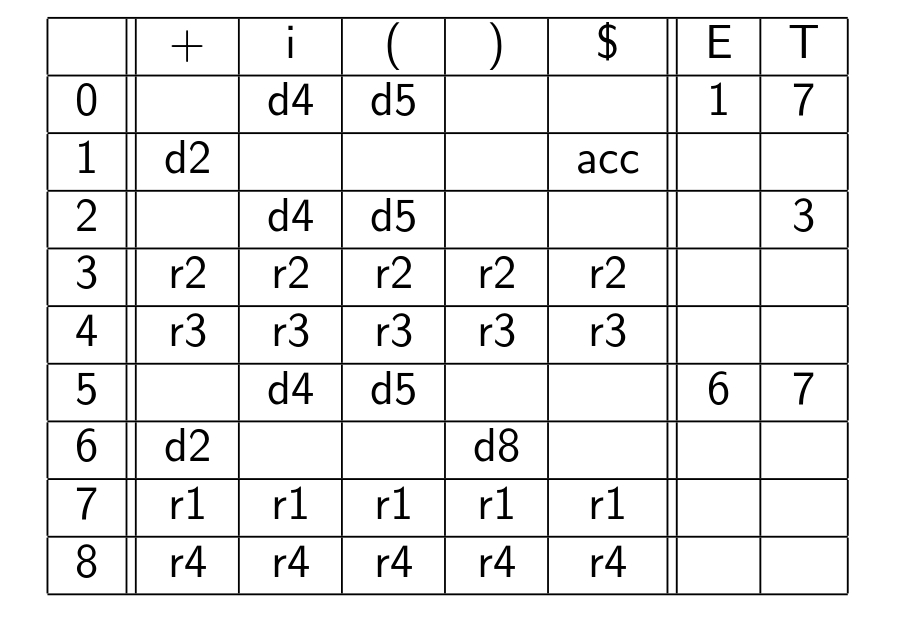
\includegraphics[scale=0.3]{img/tablaanallr0.jpg}
\end{center}

En la cual vemos que se indica la acción a realizar según el estado en el que nos encontremos y el símbolo de entrada que leamos.

Así, para realizar el análisis de una entrada nos basta con utilizar esta tabla y una pila en la que vayamos guardando las acciones que vamos realizando.

A la hora de analizar una entrada realizamos los siguientes 5 tipos de acciones:
\begin{itemize}
\item ERROR: si llegamos a una casilla en blanco de la tabla se deduce que la entrada es incorrecta.
\item Desplazar (símbolo terminal): Avanzamos un símbolo en la entrada y lo introducimos en la pila junto con el número del estado al que saltas. Corresponde a las casillas dx, siendo x el estado al que saltamos.
\item Reducir: Sacar de la pila la parte derecha de la regla (doble de símbolos de los que tiene la parte derecha ya que sacamos símbolo y número de estado al que saltó). Tras la reducción se considera que volvemos al estado $S_0$ con símbolo de entrada el de la parte izquierda de la regla que se acaba de reducir. Corresponde a las casillas rx, siendo x la regla de la gramática que reducimos.
\item Ir a (desplazamiento de símbolo no terminal). Saltar al estado indicando introduciendo en la pila el no terminal y el estado al que se salta. Se aplica justo después de realizar una reducción. No se avanza por tanto en la cadena de entrada. Corresponde a las casillas de la tabla en la que hay solo un número (estado al que saltamos).
\item Aceptar: Se acepta el símbolo e entrada si llegamos al estado de aceptación $S_{acc}$.
\end{itemize}

La siguiente tabla recoge el resultado detallado del análisis de la entrada (por comodidad mostramos en análisis mejorado, guardando en la pila el estado en que nos encontramos):
\[i+i+i\$\]
\begin{tabular}{| c | c | c | c | c | c |}
\hline
Instante & Entrada &  Pila2 & Acción \\
\hline
0 & i+i+i\$ & 0 & d4: desplazar i, saltar a 4\\
\hline
1 & +i+i\$ & 0i4 & r3: Reducción con regla 3, T -> i \\
\hline
2 & +i+i\$ & 0& 7: desplazar T, ir a 7 \\
\hline
3 & +i+i\$ & 0T7 & r1: reducción E -> T\\
\hline
4  & +i+i\$ & 0 & 1: desplazar E, ir a 1 \\
\hline
5 & +i+i\$  & 0E1 & d2: desplazar +, saltar a 2\\
\hline
6 & i+i\$  & 0E1+2 & d4: desplazar i, saltar a 4\\
\hline
7 & +i\$ & 0E1+2i4 & r3: reducción T -> i \\
\hline
8 & +i\$ & 0E1+2 & 3: desplazar T, ir a 3 \\
\hline
9 & +i\$ & 0E1+2T3 & r2: reducción E -> E+T \\
\hline
10 & +i\$ & 0 & 1: desplazar E, ir a 1 \\
\hline
11 & +i\$ & 0E1 & d2: desplazar +, saltar a 2 \\
\hline
12 & i\$ & 0E1+2 & d4: desplazar i, saltar a 4 \\
\hline
13 & \$ & 0E1+2i4 & r3: reducción T -> E\\
\hline
14 & \$ & 0E1+2 & 3: desplazar T, ir a 3 \\
\hline
15 & \$ & 0E1+2T3 & r2: reducción E -> E+T \\
\hline
16 & \$ & 0 & 1: desplazar E, ir a 1 \\
\hline
17 & \$ & 0E1 & Acepar: desplazas \$ y saltas a $S_{acc}$ \\
\hline
\end{tabular}
\end{example}

\begin{example}
Veamos un ejemplo del análisis de una expresión que termina en error:

\begin{center}
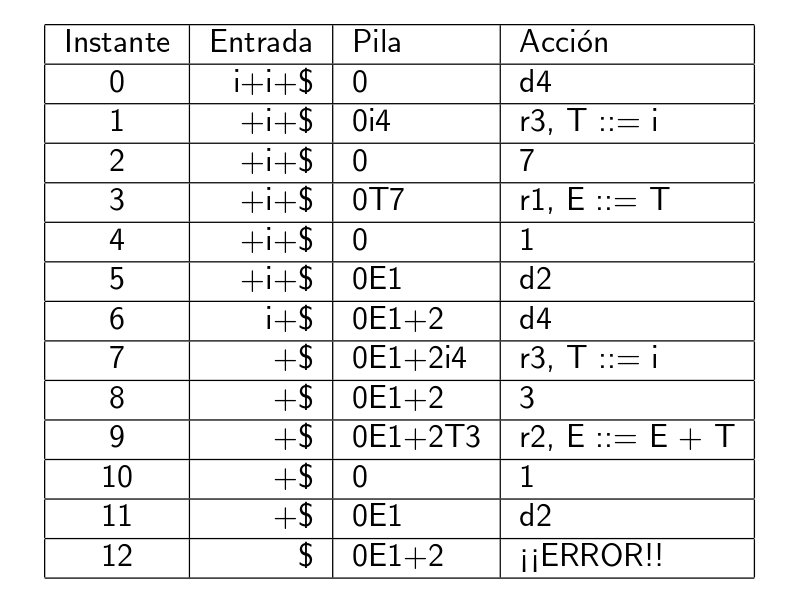
\includegraphics[scale=0.3]{img/tablaanallr0error.jpg}
\end{center}
\end{example}

\subsubsection{Conflictos, y herramientas para solucionarlos}
Vamos a definir nuevos conceptos que pondremos en práctica en esta sección.

Las tablas LR(0) no son suficientemente potentes para representar todo tipo de gramáticas. Podemos encontrarnos dos tipos de conflictos:

\begin{itemize}
\item Conflicto desplazamiento/reducción: Se producen cuando te encuentras en un estado final y además de la reducción, existe la posibilidad de desplazar.
\item Conflicto reducción/reducción: Se producen cuando te encuentras en un estado final y puedes realizar una reducción utilizando dos reglas diferentes.
\end{itemize}

Para solucionar estos conflictos definimos primero(x) y siguiente(x):

\begin{defn}[Primero(A)]
El primero de A es el conjunto de terminales que pueden aparecer al principio de una cadena derivada de A.
\end{defn}

Veamos cómo calcular el primero de A. Para ello observamos que existen tres diferentes casos para una regla de la forma $A \rightarrow α$:
\begin{enumerate}
\item $α \in T$ (Si α es un símbolo terminal):  primero(A)=α
\item $α \in N$ (Si α es un símbolo no terminal): primero(A)=primero(α)

%\item $α = α_1α_2...α_n \in T \cup %N$: Este sería el caso más %interesante. Vamos a construir %primero(A) por partes.
%\begin{verbatim}
%primero(A) añadimos primero(α1)-{λ}
%si λ pertenece a primero(α1):
%    añadimos primero(α2)-{λ}
%    si λ pertenece a primero(α2):
%        añadimos primero(α3)-{λ}
\end{enumerate}

Veamos un ejemplo
\begin{example}
Dada la gramática:
\begin{itemize}
\item $E \rightarrow TE'$
\item $E' \to +TE'$
\item $E' \to λ$
\item $T \to FT'$
\item $T' \to *FT'$
\item $T' \to λ$
\item $F \to (E)$
\item $F \to i$
\end{itemize}

Vamos a calcular el primero de algunos símbolos. Por ejemplo:

primero(E')=$\{+, λ\}$

primero(T')=$\{*, λ\}$

primero(F)=$\{(, i\}$

primero(T)=$\{(, i\}$

primero(E)=$\{(, i\}$
\end{example}

\begin{example}
Si tuviéramos la misma gramática que en el apartado anterior cambiando la regla $T' \rightarrow λ$ por $T' \rightarrow λT$, entonces:

primero(T')=$\{*,λ, (, i\}$
\end{example}



\begin{defn}[Siguiente(A)]
Dada una gramática, el siguiente de un elemento, A, es el conjunto de símbolos terminales que pueden aparecer justo después de A en alguna forma sentencial derivada del axioma.
\end{defn}

Para calcularlo formalmente, dada una regla $\appl{}{X}{\alpha A \{\beta_1,\beta_2,...\}}$, con $\alpha, \beta_i \in \sum^*$
\begin{enumerate}
\item añadimos primero($\beta_1$) $\setminus \lambda$  a siguiente(A).
\item si $\lambda \in$ primero($\beta_1$), repetimos (1) con $\beta_2$.
\end{enumerate}
\begin{itemize}
\item iteramos hasta que $\lambda \notin$ primero($\beta_j$) o se acaben los símbolos a su derecha.
\item si se acaban los símbolos a su derecha, añadimos siguiente(X) a siguiente(A).
\item si el algoritmo te lleva a que en siguiente de un símbolo se debe unir siguiente de ese mismo símbolo, se ignora.
\end{itemize}

\obs $\$ \in $ Siguiente(axioma) siempre (Al formar la gramática extendida). En este caso como el axioma es E, y ya existe un E', habría que definir una nueva regla del tipo $E'' \rightarrow E\$$

Veamos un ejemplo para poner en práctica lo aprendido:

\begin{example}
Considerando la misma gramática del ejemplo anterior, tenemos:

E es el axioma, y por tanto tenemos que:

siguiente(T)=primero(E') $\cup$ siguiente(E') $\cup$ siguiente(E) = $\{ +, ), \$\}$

siguiente(E')=siguiente(E) = $\{ ), \$ \}$

siguiente(E)=$\{ ), \$\}$

siguiente(F)=primero(T') $\cup$ siguiente(T) $\cup$ siguiente(T') = $\{ +, *, ), \$ \}$

siguiente(T')=siguiente(T) = $\{ +, ), \$ \}$
\end{example}


\subsection{Tablas SLR(1)}

Las tablas de análisis SLR(1) surgen para solucionar los conflictos desplazamiento/reducción. Lo vemos con un ejemplo:
\newpage
\begin{example}
Definimos la siguiente gramática extendida para aplicarle la tabla de análisis LR(0):

\begin{itemize}
\item (0) B' $\rightarrow$ B \$
\item (1) B $\rightarrow$ bD;Ef
\item (2) D $\rightarrow$ d
\item (3) D $\rightarrow$ D;d
\item (4) E $\rightarrow$ e
\item (5) E $\rightarrow$ e;E
\end{itemize}

Genera el siguiente autómata:
\begin{center}
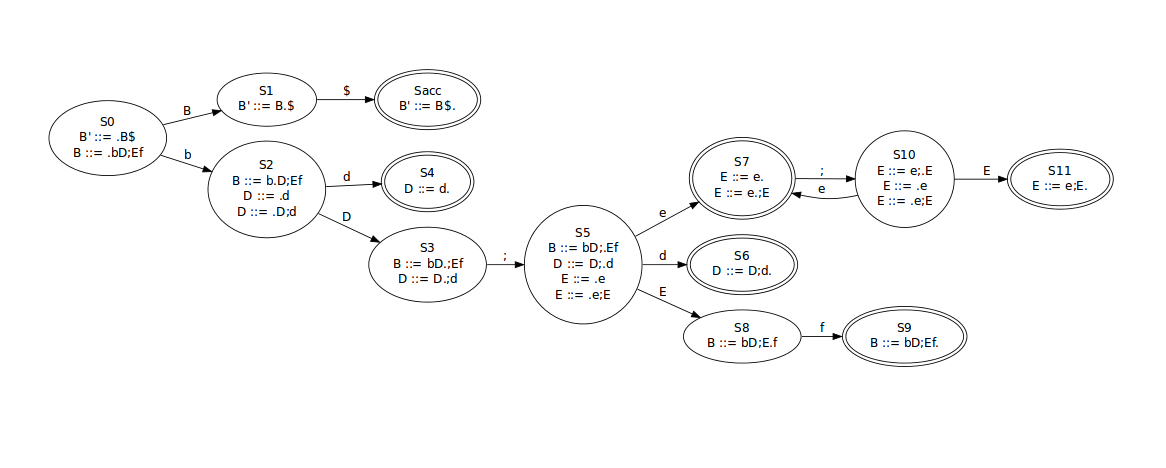
\includegraphics[scale=0.4]{img/automatalr0conflicto.jpg}
\end{center}

En el cual podemos observar que en el estado final $S_7$ tenemos dos posibles acciones si entra un ';', la de reducir (por ser estado final y encontrarse el '.' a la derecha de la regla) o la de desplazar al estado $S_{10}$

Por tanto nos quedaría la siguiente tabla de análisis LR(0):

\begin{center}
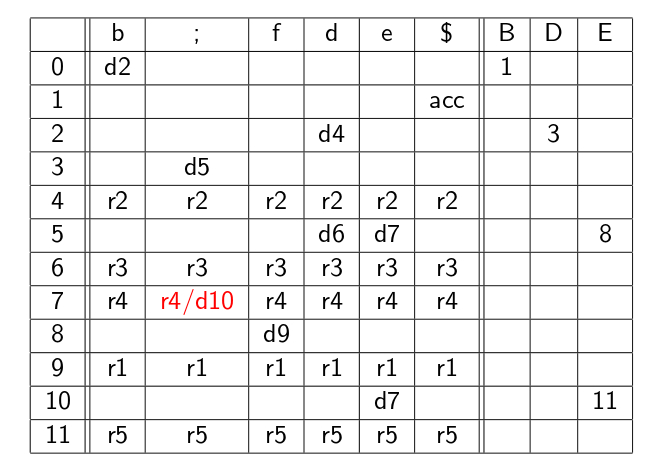
\includegraphics[scale=0.3]{img/tablaanalisislr0conflicto.jpg}
\end{center}
\end{example}
Concluimos que no es por tanto un autómata LR(0) ya que tenemos conflictos que debemos solucionar. Para ello usaremos SLR(1).

\begin{defn}[Tabla SLR(1)]
Tabla que mejora la tabla de análisis LR(0) modificando las transiciones de los estados finales del autómata.

En el caso de LR(0) realizaban una reducción siempre, mientras que en SLR(1) se específica cuándo hay que realizar una reducción, cuándo un desplazamiento, y cuándo vamos a un estado de error.
\end{defn}

Por tanto el autómata quedará igual a simple vista (sólo que ahora habra más transiciones a estados de error aunque estas no aparezcan dibujadas). Los cambios los mostraremos en la tabla de análisis.

La idea principal del análisis SLR(1) es que sólo aplicaremos las reducciones de reglas de la froma $X \rightarrow $ algo, delante del \textbf{Siguiente(X)}.

Vamos a calcular los elementos siguientes de los no terminales B, D y E.

\begin{itemize}
\item siguiente(B) $\rightarrow$ {\$}, por tanto las reducciones de B sólo se producirán delante del símbolo \$.
\item siguiente(D) $\rightarrow$ {;}, por tanto las reducciones de B sólo se producirán delante del símbolo \$.
\item siguiente(E) $\rightarrow$ {f}, por tanto las reducciones de B sólo se producirán delante del símbolo \$.
\end{itemize}

Se eliminan así los conflictos, quedando la tabla de análisis de la siguiente manera:

\begin{center}
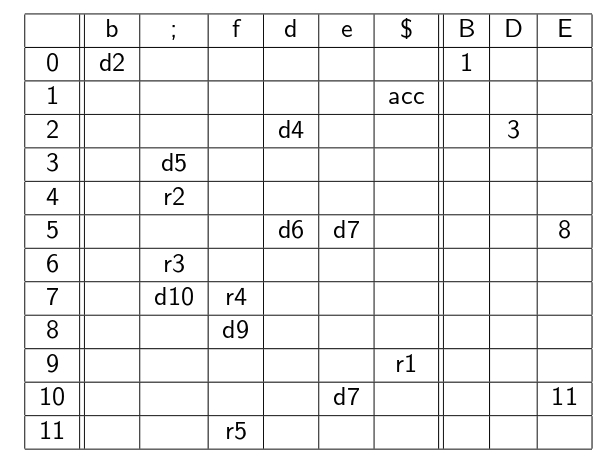
\includegraphics[scale=0.4]{img/tablaanalisisslr1.jpg}
\end{center}

Como podemos observar, en el estado S7, se reduce siguiendo la regla (4) (ver las reglas de la gramática definidas al principio del ejemplo), pero sólo si el siguiente elemento de la entrada es una f, ya que siguiente(E)={f}.
\newpage
Conclusión: Para realizar una tabla de análisis SLR(1) basta con:
\begin{enumerate}
\item Hacer la tabla de análisis LR(0).
\item Calcular los elementos siguientes de los símbolos no terminales.
\item Modificar las filas de la tabla que correspondan a estados finales. Poniendo huecos en blanco en todas las casillas salvo en aquellas en las que haya desplazamiento y aquellas en las que realmente reduzcamos, es decir, en las que el siguiente elemento del que vayamos a reducir coincida con el de la entrada.
\end{enumerate}


\subsection{Tablas LR(1)}
Las tablas LR(1) surgen para corregir los conflictos desplazamiento/reducción que no es capaz de solventar el análisis SLR(1).

Veamos dos ejemplos en los que el análisis SLR(1) falla:

\begin{example}
Definimos la siguiente gramática extendida para aplicarle la tabla de análisis SLR(1):

\begin{itemize}
\item (0) E' $\rightarrow$ E \$
\item (1) E $\rightarrow$ E+E
\item (2) E $\rightarrow$ E*E
\item (3) E $\rightarrow$ i
\end{itemize}

Genera el siguiente autómata:
\begin{center}
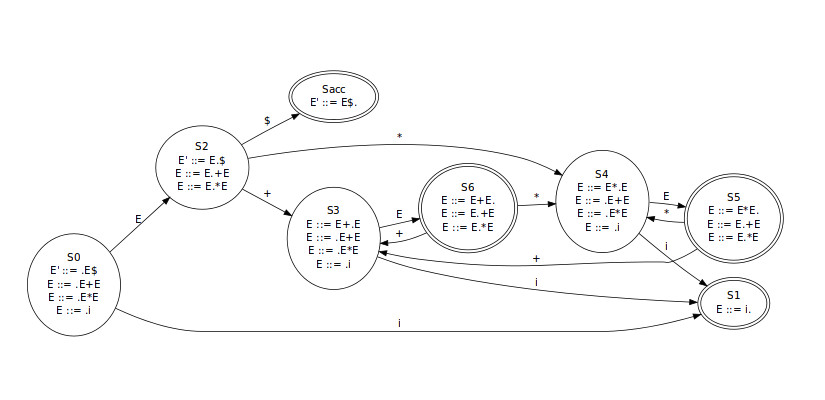
\includegraphics[scale=0.5]{img/automataslr1conflicto.jpg}
\end{center}

En el cual podemos observar que en el estado final $S_6$ podríamos desplazar o reducir para los símbolos '+' y '*'. Ya que siguiente(E)=$\{+,*\$\}$.

\newpage
Por tanto nos quedaría la siguiente tabla de análisis:

\begin{center}
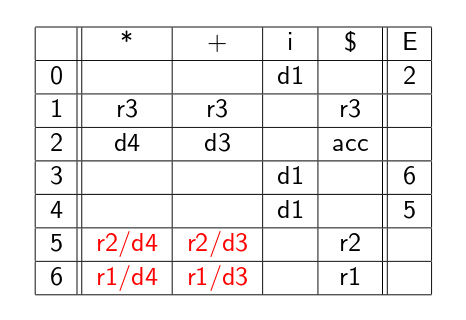
\includegraphics[scale=0.4]{img/tablaanalisisslr1conflicto.jpg}
\end{center}
\end{example}

\begin{example}
Definimos la siguiente gramática extendida para aplicarle la tabla de análisis SLR(1):

\begin{itemize}
\item (0) S' $\rightarrow$ S \$
\item (1) S $\rightarrow$ xb
\item (2) S $\rightarrow$ A
\item (3) A $\rightarrow$ aAb
\item (4) A $\rightarrow$ x
\end{itemize}

Genera el siguiente autómata:
\begin{center}
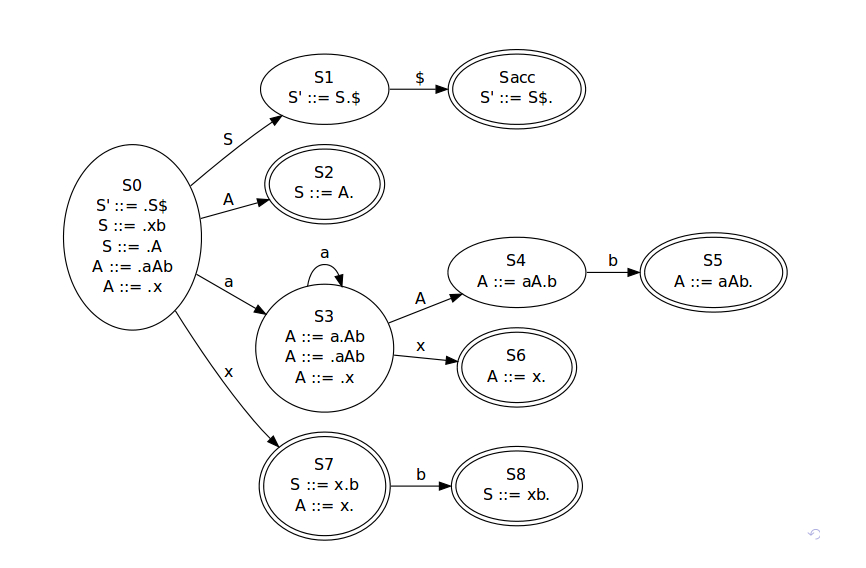
\includegraphics[scale=0.5]{img/automataslr1c1.jpg}
\end{center}

En el cual vuelve a ocurrir algo parecido a lo del ejemplo anterior. En este caso tenemos que:
\begin{itemize}
\item siguiente(S)=$\{\$\}$
\item siguiente(A)=$\{b,\$\}$
\end{itemize}
Por tanto nos quedaría la siguiente tabla de análisis:

\begin{center}
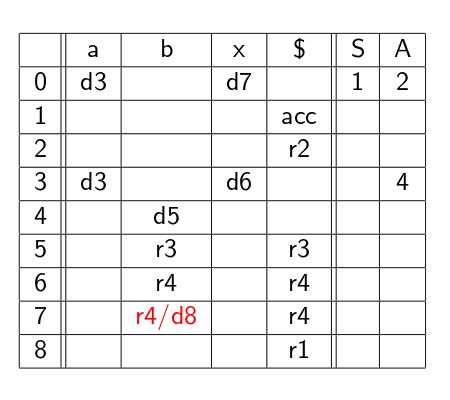
\includegraphics[scale=0.4]{img/tablaanalisisslr1c1.jpg}
\end{center}
\end{example}

Mediante el análisis SLR(1) no añadíamos ningún estado más al autómata, únicamente cambiábamos la tabla de análisis. Ahora, con LR(1) vamos a añadir más estados a nuestro autómata. Así, para formar un autómata LR(1) realizamos los siguientes pasos:

\begin{enumerate}
\item Ahora la gramática extendida no va a tener una regla que sea $S' \rightarrow S\$$ sino que esta regla será $S' \rightarrow S\{\$\}$.
\item Vamos a formar cada estado como en LR(0), poniendo un '.' delante del símbolo que estamos evaluando y \textbf{cerrando} ese símbolo como ya explicamos anteriormente.
\item A cada regla que aparezca en cada estado del autómata se deberá añadir entre corchetes lo que llamaremos el \textbf{símbolo de adelanto}.

Este símbolo es el siguiente(X) si tenemos $X \rightarrow ABC...$, es decir, el siguiente del símbolo no terminal situado a la izquierda de la regla.

\textbf{Esto es algo más complicado de lo que parece. Completar}

\end{enumerate}

Como resultado, tendremos un mayor número de estados ya que si el símbolo de adelanto cambia, habrá que definir un nuevo estado.

\begin{example}
Usando la gramática del ejercicio anterior, generamos el siguiente autómata usando LR(1):

\begin{center}
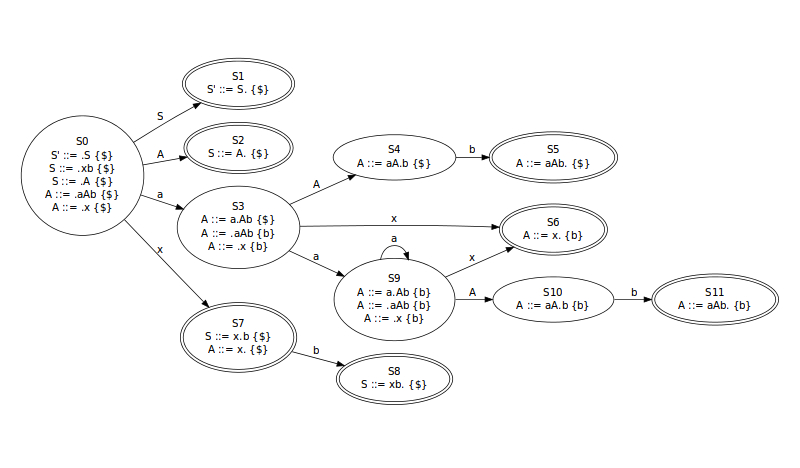
\includegraphics[scale=0.65]{img/automatalr1.jpg}
\end{center}
\obs En este ejemplo hay una errata. En los estados $S_0$, $S_3$ y $S_7$ la regla $A::== .Ab \{\$\}$ debería ser $A::== .Ab \{b\}$, puesto que Siguiente(A) =$\{b\}$ y la regla $A::== .x \{\$\}$ debería ser $A::== .x \{b\}$

Como podemos observar, en este autómata se eliminan los conflictos que teníamos antes. Nos fijamos en la clave de esto.

Nos quedaría la siguiente tabla de análisis:

\begin{center}
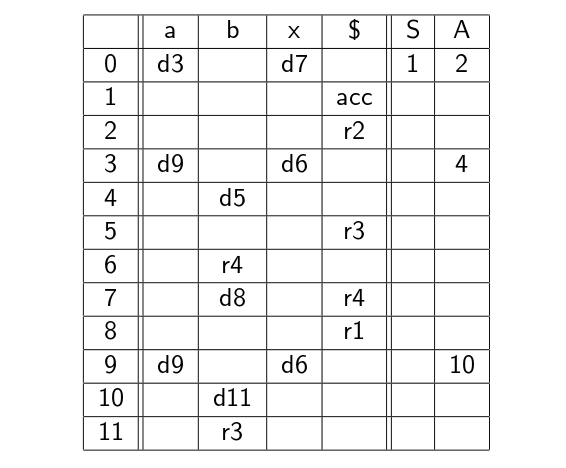
\includegraphics[scale=0.4]{img/tablaanalisislr1.jpg}
\end{center}
\end{example}

\subsection{Tablas LALR(1)}

El análisis LALR(1) supone reducir el tamaño de la tabla de análisis de LR(1), a cambio de la posibilidad de aparición de conflictos reducción/reducción.

Debemos tener en cuenta que buena parte de la complejidad del algoritmo recae en el coste de procesar la entrada siguiendo un autómata y que, cuando menor sea el mismo menor será el coste.

La principal diferencia que aporta el análisis LALR(1) consiste en la agrupación de estados finales que sólo difieran en los símbolos de adelanto.

Veamos como transformar un autómata LR(1) en un autómata LALR(1).

% \includepdf[frame=true, noautoscale=true, delta=10 10, nup=2x4,pages={32-39}, scale=0.72]{pdf/lrpres.pdf}
% \includepdf[frame=true, noautoscale=true, delta=10 10, nup=2x4,pages={40-41}, scale=0.72]{pdf/lrpres.pdf}



\section{Análisis descendente}
Vamos a estudiar cómo se desarrollan los algoritmos de análisis descendente.

Ya los mencionamos anteriormente pero, para ver cómo funcionan, vamos a realizar algunos ejemplos por fuerza bruta, para captar la idea del asunto.

\begin{example}
Empezaremos por una gramática sencillita:
\begin{itemize}
\item S $\rightarrow$ aSb
\item S $\rightarrow$ ab
\end{itemize}
y trataremos de ver si la cadena $aabb$ se deriva de esta gramática.

Para empezar a estudiar el ejemplo, debemos tener en cuenta dos máximas del análisis descendente:

\textbf{La cadena se lee desde la izquierda}

\textbf{Realizaremos siempre derivaciones Left most}

Vamos a realizar el ejercicio por \textit{fuerza bruta}.
\begin{verbatim}
Para empezar derivamos el axioma con la primera regla (en realidad daría igual
cual coger).
Obtenemos por tanto S->aSb y vemos que es compatible con la cadena buscada.

Tomamos ahora el elemento no terminal situado más a la izquierda y lo derivamos.
Obtenemos así S->aSb->aaSbb que vemos que es compatible con la entrada.

Derivamos una vez más el siguiente elemento no terminal más a la izquierda.
En esta ocasión llegamos a S->...->aaaSbbb que ya no es compatible con la
cadena de modo que deshacemos la última operación.

Tratamos de aplicar la segunda regla.
Así obtenemos S->...->aaabbb que tampoco es compatible por lo que volvemos
a deshacer el último paso.

Nos hemos quedado sin reglas por aplicar, de modo que debemos deshacer una
acción más. Volvemos al estado S->aSb y tratamos de aplicar la segunda regla:
Llegamos a S->aSb->aabb y vemos que coincide con la cadena buscada.
\end{verbatim}
\end{example}

Al explicar el algoritmo empleado hemos hecho alusión a la compatibilidad. Definámosla formalmente.

\begin{defn}[Compatibilidad]
Para comprobar si la cadena que tenemos ahora mismo es \textbf{compatible} con la cadena que estamos buscando simplemente vemos si los primeros símbolos terminales (hasta el primer no terminal) coinciden.
\end{defn}

Tal y como lo hemos explicado ,el algoritmo de análisis descendente presenta dos problemas graves:
\begin{enumerate}
\item Es extremadamente ineficiente
\item Recursividad por la izquierda.

Si nos encontramos con una gramática del tipo
\begin{itemize}
\item S $\rightarrow$ b
\item S $\rightarrow$ Sb
\end{itemize}
y buscamos la cadena $abb$ entraríamos en un problema de recursión infinita pues aplicar la primera regla no nos da la solución final en ningún caso y con la segunda regla tendremos siemrpe al inicio de la cadena un símbolo que no es terminal.
\end{enumerate}

Para clasificar las gramáticas según puedan causarnos o no este problema vamos a definir un nuevo concepto

\begin{defn}[Gramática LL(1)]
Gramática en la que todas las reglas presentan en la parte derecha 1 símbolo no terminal seguido de un símbolo cualquiera (terminal o no terminal).

Además, dos reglas con la misma parte izquierda deben un terminal distinto al inicio de su parte derecha.
\end{defn}

Estas gramática son muy interesantes ya que presentan un claro determinismo, que nos evita de hacer backtracking con lo que hacen la búsqueda muy eficiente.


Veremos dos métodos para el análisis de gramáticas de este tipo pero antes debemos definir un nuevo concepto muy importante de cara al análisis descendente: \textbf{Forma normal de Greigbach}

\subsection{Forma normal de Greigbach}

\begin{defn}[Forma normal de Greigbach]
Decimos que una gramática está en forma normal de Greigbach si todas las reglas son de la forma:
\[A \rightarrow a\beta \text{ donde } a \in T, \ \beta \in N^*\]
\end{defn}

\obs Todas las gramáticas pueden expresarse en forma normal de Greigbach.

Una vez que una gramática está expresada de esta forma, comprobamos si es, además, LL(1) y si es así ya lo tenemos.

Vamos a ver cómo tratar una gramática que no esté expresada en forma normal de Greigbach. En estos casos debemos solucionar, antes de nada, los dos problemas que nos impiden que la gramática esté en esta forma normal

\begin{enumerate}
\item \textbf{Eliminación de reglas recursivas por la izquierda}

Dada una gramática de la forma
\begin{itemize}
\item A $\rightarrow$ A$\beta$
\item A $\rightarrow$ α
\end{itemize}
la convertimos en otra
\begin{itemize}
\item A $\rightarrow$ αX
\item X $\rightarrow$ $\beta$X|λ
\end{itemize}

\item \textbf{Eliminar símbolos no terminales del principio de la parte derecha de las reglas.}


Vamos a clasificar las reglas en tres tipos:
\begin{enumerate}
\item $A \rightarrow aZ$
\item $A_i \rightarrow A_jα$ con $A_i$ precediendo a $A_j$
\item $A_i \rightarrow A_jα$ con $A_j$ precediento a $A_i$
\end{enumerate}

El algoritmo a seguir sería:
\begin{enumerate}
\item Dejamos las reglas de Tipo a) como están.
\item Eliminamos las reglas de Tipo c), empezando con aquellas cuyo símbolo de la parte derecha tiene mayor precedencia
\item Eliminamos las reglas de Tipo b), empezando con aquellas cuyo símbolo de la parte izquierda tenga menor precedencia.
\end{enumerate}
\item \textbf{Eliminar símbolos terminales de más.}

Para ello, dada una regla
\[A \rightarrow abX\]

pasamos a dos reglas:
\[A \rightarrow aBX\]
\[B \rightarrow b\]

\item \textbf{Eliminar reglas λ}
\item \textbf{Eliminar indeterminismo}

Dadas reglas de la forma
\begin{enumerate}
\item $A \rightarrow aZ$
\item $A \rightarrow aB$
\end{enumerate}
sacamos factor común y llegamos a
\begin{enumerate}
\item $A \rightarrow aW$
\item $W \rightarrow B$
\item $W \rightarrow Z$
\end{enumerate}

Tras este paso vemos si aparecen reglas recursivas. En caso afirmativo, las eliminamos nates de seguir.
\item \textbf{Volvemos al primer paso y repetimos}

\obs Si la gramática no es LL(1) este algoritmo no converge
\end{enumerate}

Veamos un ejemplo de cómo aplicar este algoritmo
\begin{example}
Tomamos la gramática:
\begin{itemize}
\item $E \rightarrow E+T$
\item $E \rightarrow T$
\item $T \rightarrow T*T$
\item $T \rightarrow F$
\item $F \rightarrow i$
\end{itemize}
Primero eliminamos las reglas recursivas por la izquierda y nos quedamos en:
\begin{itemize}
\item $E \rightarrow TX$ (tipo 2)
\item $X \rightarrow +TX|λ$ (tipo 1)
\item $T \rightarrow FY$ (tipo 2)
\item $Y \rightarrow *TY|λ$ (tipo 1)
\item $F \rightarrow i$ (tipo 1)
\end{itemize}
donde hemos indicado el tipo de cada regla, preparándonos así para el paso siguiente.

Ahora tenemos que eliminar los símbolos no terminales del principio de la parte derecha de las reglas. Para ello aplicamos las siguientes transformaciones
\begin{itemize}
\item $T \rightarrow FY \ \implies T \rightarrow iY$
\item $E \rightarrow TX \ \implies E \rightarrow FYX \implies F \rightarrow iYX$
\end{itemize}
en el orden exacto en que se han indicado.

El resultado por el momento es:
\begin{itemize}
\item $E \rightarrow iYX$
\item $X \rightarrow +TX$
\item $X \rightarrow λ$
\item $T \rightarrow iY$
\item $Y \rightarrow *TY$
\item $Y \rightarrow λ$
\item $F \rightarrow i$
\end{itemize}

Pero a esta gramática aún le falta algo para ser de Greibach, tenemos que eliminar las transiciones vacías, obteniendo:
\begin{itemize}
\item $E \rightarrow iYX$
\item $E \rightarrow iY$
\item $E \rightarrow iX$
\item $E \rightarrow i$
\item $X \rightarrow +TX$
\item $X \rightarrow +T$
\item $T \rightarrow iY$
\item $T \rightarrow i$
\item $Y \rightarrow *TY$
\item $Y \rightarrow *T$
\item $F \rightarrow i$
\end{itemize}
El método seguido se basa en la duplicación de aquellas reglas que contengan $Y$ ó $X$ (los no terminales que ocasionaban transiciones λ) añadiéndoles una opción sin esas variables, que es lo que obtendríamos si empleásemos la derivación λ
\end{example}

El último paso llevado a cabo en el ejemplo (eliminación de reglas λ) no es siempre necesario.

Recordemos que queríamos saber si una gramática era de forma normal de Greibach con el fin de reconocer si era LL(1). Desde el último estado que hemos alcanzado en la gramática, para convertirla en una gramática LL(1) deberíamos eliminar los no terminales que aparecen repetidos en numerosas reglas.

Sin embargo, desde el paso anterior tendríamos directamente que la gramaica es LL(1).

La pregunta que surge ahora está clara:

\subsection{¿Cuándo nos interesa eliminar las transiciones λ?}
En general, nos interesará eliminar las transiciones λ siempre que al hacerlo no estemos generando una gramática no LL(1). Es decir, queremos eliminar estas transiciones sin dar lugar a gramáticas no deterministas.

En general,
\[\text{ primero}(X) \cap \text{ siguiente}(X) = \emptyset \implies \ X \rightarrow λ\text{ no molesta para LL(1)}\]

En el ejemplo anterior ninguna de las reglas λ nos molestaban de modo que podíamos prescindir del último paso para garantizar que la gramática es LL(1)

\subsection{Analisis LL(1) usando la tabla}
El algoritmo a seguir es el siguiente
\begin{enumerate}
\item Inicializamos la pila con S\$
\item Inicializamos la entrada al primer elemento de la cadena
\item Comparamos la pila con la entrada
\begin{enumerate}
\item pila=entrada=\$ \textbf{FIN}
\item pila contiene x$\in T$
\begin{enumerate}
\item x = entrada $\implies$ \textbf{desplazamos entrada y pop}
\item x $\neq$ entrada $\implies$ \textbf{ERROR}
\end{enumerate}
\item pila contiene $x \in N \implies$ \textbf{saco x de la pila y meto $\beta$}.
\end{enumerate}
\end{enumerate}

Veamos un pequeño ejemplo de cómo aplicar este algoritmo.
\begin{example}
Consideremos la gramática:
\begin{itemize}
\item $S \rightarrow E \$$
\item $E \rightarrow TE'$
\item $E'\rightarrow +TE'$
\item $E'\rightarrow λ$
\item $T \rightarrow FT'$
\item $T' \rightarrow *FT'$
\item $T' \rightarrow λ$
\item $F \rightarrow i$
\item $F \rightarrow (E)$
\end{itemize}
Y vamos a analizar con ella la entrada
\[i+i*i\$\]

La tabla queda:
%TODO copiar tabla
\begin{center}
\begin{tabular}{| c | c | c | c | c | c | c |}
\hline
Simbolo & + & * & i & ( & ) & \$ \\
\hline
E &  &  & E $\rightarrow$TE' & $E\rightarrow TE'$ & & \\
\hline
E' & $E'\rightarrow +TE'$ & & & & $E'\rightarrow λ$ & $E'\rightarrow λ$\\
\hline
T & &  & $T \rightarrow FT'$ & $T \rightarrow FT'$ & & \\
\hline
T' & $T' \rightarrow *FT'$ & $T' \rightarrow λ$ & & & $T' \rightarrow λ$ & $T'\rightarrow λ$  \\
\hline
F & & & $F\rightarrow i$ & $F\rightarrow (E)$ & &\\
\hline
\end{tabular}
\end{center}

y el análisis resulta:
\begin{center}
\begin{tabular}{| c | c | c | c |}
\hline
0 & i+i*i\$ & S\$ & derivar E$\rightarrow$TE' \\
\hline
1 & i+i*i\$ &  TE'\$ & derivar T $\rightarrow$ FT' \\
\hline
2 & i+i*i\$ &  FT'E'\$ & derivar F$\rightarrow$i \\
\hline
3 & i+i*i\$ &  iT'E'\$ & desplazar entrada \\
\hline
4 & +i*i\$ &  T'E'\$ & derivar T' $\rightarrow$ λ \\
\hline
5 & +i*i\$ &  E'\$ & derivar E' $\rightarrow$ TE' \\
\hline
6 & +i*i\$ &  +TE'\$ & desplazar \\
\hline
7 & i*i\$ &  TE'\$ & dderivar T $\rightarrow$ FT' \\
\hline
8 & i*i\$ &  FT'E'\$ & derivar F $\rightarrow$ i \\
\hline
9 & i*i\$ &  iT'E'\$ & desplazar \\
\hline
10 & *i\$ &  T'E'\$ & T' $\rightarrow$ *FT' \\
\hline
11 & *i\$ &  *FT'E'\$ & desplazar \\
\hline
12 & i\$ &  FT'E'\$ & F $\rightarrow$ i \\
\hline
13 & i\$ &  iT'E'\$ & desplazar \\
\hline
14 & \$ &  T'E'\$ & T' $\rightarrow$ λ \\
\hline
15 & \$ &  E'\$ & E' $\rightarrow$ λ \\
\hline
16 & \$ &  \$ & OK \\
\hline
\end{tabular}
\end{center}
\end{example}

\begin{example}
Consideremos la gramática:
\begin{itemize}
\item $P \rightarrow iEtPP' \$$
\item $P \rightarrow a$
\item $P'\rightarrow EP$
\item $P'\rightarrow λ$
\item $E \rightarrow b$
\end{itemize}
Vamos a construir ahora la tabla de análisis asociado.

Para ello tenemos que ver cuál es el siguiente de cada elemento no terminal y dejar claro en la tabla que sólo aplicamos la reducción delante del siguiente

La tabla de análisis asociada sería:
\begin{center}
\begin{tabular}{| c | c | c | c | c | c | c |}
\hline
Simbolo & a & t & e & b & i & \$ \\
\hline
P &  $P \rightarrow a$&  & &  &  $P \rightarrow iEtPP'$ & \\
\hline
P' & & & $P' \rightarrow  EP$   $ P' \rightarrow λ$ & & &  $ P' \rightarrow λ$ \\
\hline
E & &  &  & $E \rightarrow b$ & & \\
\hline
\end{tabular}
\end{center}

Como podemos observar, esta gramática no es LL(1)
\end{example}

Vamos a hacer incapié en la diferencia entre gramática LL(1) y lenguaje LL(1)
\begin{defn}[Gramática LL(1)]

Gramática cuya tabla de análisis LL(1) no presenta conflictos
\end{defn}

\begin{defn}[Lenguaje LL(1)]

Lenguaje para el cual existe una gramática LL(1) que lo genera
\end{defn}

\begin{example}
La gramática
\begin{itemize}
\item $ S \rightarrow aSb$
\item $ S\rightarrow ab$
\end{itemize}
no es una gramática LL(1), cosa que podemos comprobar construyendo su tabla de análisis LL(1). Sin embargo, su lenguaje asociado si que es LL(1) ya que podemos transformarla en
\begin{itemize}
\item $ B \rightarrow b$
\item $ S \rightarrow aW$
\item $ W \rightarrow aWb$
\item $ W \rightarrow b$
\end{itemize}
que si es LL(1) (de nuevo lo comprobamos construyendo su tabla de análisis LL(1)).
\end{example}


\subsection{Análisis LL(2) usando la tabla}
La principal diferencia del análisis LL(2) respecto al LL(1) radica en que ahora vamos a tomar \textbf{dos símbolos de adelanto}

Veámoslo para el caso particular de la gramática
\begin{itemize}
\item S $\rightarrow$ aSb
\item S $\rightarrow$ ab
\end{itemize}

En este caso sería tremendamente sencilla la tabla de símbolos:
\begin{center}
\begin{tabular}{| c | c | c |}
\hline
Simbolo & aa & ab \\
\hline
S &  S $\rightarrow$ ab &  S $\rightarrow$ aSb \\
\hline
\end{tabular}
\end{center}


Pero aún quedan casos en los que no podemos resolver los conflictos ni usando LL(2).

Por ejemplo, en la gramática
\begin{itemize}
\item FUNCION -> TIPO ID (ARGS);
\item FUNCION -> TIPO ID (ARGS) \{CUERPO\}
\item ARGS -> λ
\item ARGS -> ARG ARGS
\item TIPO -> int | float
\item ARG -> ID
\item ID -> $(a+...+z)(a+...+z)^*$
\end{itemize}

A la hora de trabajar con la regla \textbf{FUNCION -> TIPO ID (ARGS)} no sabemos cuántos argumentos vamos a encontrar.

La solución para este problema pasa por usar expresiones regulares, lo que nos lleva al análisis LL(*)

\subsection{Análisis LL(*)}
Consiste en emplear expresiones regulares en lugar de símbolos de adelanto.

Continuando con el ejemplo anterior, para resolver el problema con LL(*) consideramos la expresión regular:
\[r=(int+float).(a-z)^+."(".[(a-z)^+]*.")"\]
y la tabla quedaría (para la regla que causaba el problema)
\begin{center}
\begin{tabular}{| c | c | c |}
\hline
Símbolo & r.";" & r."ε" \\
\hline
FUNCION & FUNCION -> TIPO ID (ARGS); &  FUNCION -> TIPO ID (ARGS) \{CUERPO\} \\
\hline
\end{tabular}
\end{center}
En este caso no hay problemas pues es bastante sencilla la tabla mostrada. No obstante, en un caso más general sería necesario cuidar que no se solapen las expresiones regulares empleadas en el análisis.

%%%%%%%%%%%%%%%%%%%%%%%%%%%%%%%%%%%%%%%%%%%%%%%%%%%%%%
\appendix
\chapter{Ejercicios}
% -*- root: ../TIM.tex -*-
\section{Ejercicios}
\subsection{Hoja 1}
\begin{problem}[5]
Dada una sucesión $\lbrace f_n \rbrace \in R([a,b])$ que converge uniformemente a $f$, se pide demostrar que $f$ es integrable Riemann y que:
\[ \lim \int_{a}^{b} f_n = \int_{a}^{b} f \]

\solution
Supongamos que f es integrable Riemann, entonces tenemos que ver que:
\[ \forall \epsilon > 0 \ , \exists N \tq \forall n> N \ \abs{\int_a^b f_n - \int_a^b f} < \epsilon\]

Sabemos que:
\[\abs{\int_a^b f_n - \int_a^b f} \leq \abs{\int_a^b \abs{f_n -f}} dx\]

Recordemos la definición de convergencia uniforme

\begin{defn}[Convergencia\IS uniforme]
\[f_n \xrightarrow{uniforme} f \Leftrightarrow \forall \epsilon < 0, \exists N_{\epsilon} \tq \forall x \in [a,b]  \forall n \geq N_{\epsilon}, \abs{f_n (x) - f(x)} < \epsilon\]
\end{defn}

Si $n \geq N_{\frac{\epsilon}{b-a}}$ entonces, usando la definición de convergencia uniforme:

\[\int_a^b \abs{f_n(x) - f(x) dx} \leq \int_a^b \frac{\epsilon}{b-a}dx = \epsilon\]

Por tanto queda claro que si $f$ es integrable Riemann podemos conmutar el límite con la integral. Ahora queda ver por qué $f$ es integrable Riemann.

$f$ será integrable Riemann sii:
\[\forall \epsilon > 0 \ \exists P \tq \forall P' \prec P \]
\[\overline{J}_{P'}(f) - \underline{J}_{P'}(f) < \epsilon\]

Vamos a probarlo:
\[\overline{J}_P(f) - \underline{J}_P(f) = \sum(\sup_k f - \underset{k}{inf} f)\abs{I_k} \leq\]
\[\leq \sum\left( \abs{\sup_{k}f_n(x) - \sup_{k}f(x)} + \abs{\sup_{k}f_n(x) - \underset{k}{inf}f_n(x)} +  \abs{\underset{k}{inf}f_n(x) - \underset{k}{inf}f_n(x)} \right)\abs{I_k} \leq \]
Puesto que $f_n$ converge uniformemente a $f$ habrá un $n$ a partir del cual la distancia máxima entre $f_n$ y $f$ sea $\frac{\epsilon}{6}$ y por tanto la distancia máxima entre el supremo y el ínfimo de $f_n$ será menor que $\frac{\epsilon}{3}$
\[\leq \sum\left( \sup_{k} \abs{f_n(x) - f(x)} + \frac{\epsilon}{3} + \sup_k \abs{f_n(x) - f(x)} \right)\abs{I_k} \leq\]
Aplicando de nuevo la convergencia uniforme y tomando el máximo entre este $n$ y el calculado en el paso interior nos queda:
\[\leq \sum \left(\frac{\epsilon}{3} + \frac{\epsilon}{3} + \frac{\epsilon}{3} \right)\abs{I_k} = \sum\epsilon\abs{I_k}\]

Como hay convergencia uniforme entre $f_n$ y $f$ podemos hacer que los supremos sean tan pequeños como queramos y hacer así que el interior sumatorio quede menor que $\epsilon \abs{I_k}$

Puesto que $\epsilon$ es un número cualquiera podemos hacerlo tan pequeño como queramos haciendo que el último sumatorio escrito tienda a 0.

\end{problem}

\begin{problem}[6]

Sea $\lbrace f_n \rbrace$ una sucesión monótona creciente de funciones continuas en un intervalo $I=[a,b]$ que convergen en dicho intervalo a otra función continua $f$. Demuestra que entonces:
\[ lim \int_{a}^{b} f_n(x) = \int_{a}^{b} f(x) \]
\solution
Por ser funciones continuas son integrables Riemann. Si conseguimos demostrar que convergen uniformemente podemos emplear el ejercicio anterior y lo tendríamos hecho.
\end{problem}

\begin{problem}[7]
Dada la sucesión $I_k = (a_k, b_k)$ tales que $\bigcup_{k=1}^{N}~I_k~=~[a,b]$

Demostrar que:
\[b-a \leq \sum_{k=1}^N (b_k - a_k)\]

\solution
Vamos a utilizar la integral de Riemann como recomienda el ejercicio, utilizando la función indicatriz de cada intervalo $\ind_{I_k}$

Está claro que la función indicatriz del intervalo I es menor o igual que la suma de las funciones indicatrices de los intervalos. Lo cual es obvio, ya que si $x$ está en el intervalo, $x$ estará también en al menos uno de los intervalos $I_k$. Es decir:
\[\ind_{[a,b]} \leq \sum_{k=1}^{N} \ind_{I_k}\]

Utilizando la monotoneidad de la integral de Riemann podemos ``integrar a ambos lados'' obteniendo:

\[\int_{a}^{b} \ind_{[a,b]} \leq \int_{a_k}^{b_k} \sum_{k=1}^{N} \ind_{I_k}\]

Por la linealidad de la integral, podemos incluso meter la integral dentro del sumatorio
\[\int_{a}^{b} \ind_{[a,b]} \leq \sum_{k=1}^{N} \int_{a_k}^{b_k} \ind_{I_k}\]


Conociendo la integral de la función indicatriz tenemos el resultado de forma inmediata.
\[b-a \leq \sum_{k=1}^{N} ( b_k - a_k )\]

\end{problem}

\begin{problem}[9]
Dado $O\subset (a,b)$ unión numerable de intervalos disjuntos, se pide demostrar:
\[m^*(O)=\sum_{n=1}^{\infty} \abs{I_k}\]

\solution
Está claro que:
\[m^*(O) \leq \sum_{n=1}^{\infty} \abs{I_k}\]

Tenemos que demostrar la desigualdad contraria para poder concluir la igualdad.
Vamos a probar que:
\[m^*(O) \geq \sum_{n=1}^{\infty} \abs{I_k} - \epsilon\]

Puesto que sabemos que la suma infinita tiene un resultad finito (ya que $O$ es finito)
\[\forall \epsilon > 0 \exists N \tq \sum_{n=1}^N\abs{I_n} \geq \sum_{n=1}^{\infty} \abs{I_k} - \frac{\epsilon}{2}\]

Vamos a definir los intervalos $I'_n$ que serán un poco más pequeños que los $I_n$
\[\forall n=1,2,...,N \text{ definimos } I'_n=[a_n+\frac{\frac{\epsilon}{2}}{2^{n+1}}, b-\frac{\frac{\epsilon}{2}}{2^{n+1}}]\]

Ahora tenemos que:
\[\sum_{n=1}^N \abs{I'_n}=\sum_{n=1}^N\abs{I_n} - \frac{\epsilon}{2}\sum_{n=1}^{N}\frac{1}{2^n} \geq \sum_{n=1}^N\abs{I_n} - \frac{\epsilon}{2}\]

Definimos ahora el compacto:
\[K_n = \bigcup_{n=1}^N I'_n\]

Sean $J_n$ intervalos abiertos tales que $O \subset \bigcup_{n=1}^{\infty}J_n \Rightarrow K_n \subset \bigcup_{n=1}^{\infty}J_n$.

Por tanto
\[\exists N' \tq K_n \subset \bigcup_{n=1}^{N'}J_n=A_N\]

Vamos a fijarnos ahora en la medida exterior de $O$:

\[ m^*(O) = \inf\lbrace \sum_{n=1}^{\infty}\abs{J_n} \rbrace \geq \inf\lbrace \sum_{n=1}^{N'}\abs{J_n} \rbrace \geq \]
\[ \geq \inf\lbrace \int \ind_{A_N} \rbrace \geq \inf\lbrace \int \ind_{K_N} \rbrace \geq \inf\lbrace \sum_{n=1}^N\abs{I'_n} \rbrace \geq \]
\[ \geq \inf\lbrace \sum_{n=1}^N\abs{I_n} -\frac{\epsilon}{2}\rbrace \geq \inf\lbrace \sum_{n=1}^N\abs{I_n} -\epsilon \rbrace \]

Y obtenemos así la desigualdad buscada.
\end{problem}

\begin{problem}[10]
Dado un compacto K contenido en el intervalo (a,b), nos piden demostrar que:
\[m(K)<b-a\]

\solution
Consideremos la sucesión: $(a+\frac{1}{n}, b - \frac{1}{n})$, con $n >\frac{2}{b-a}$. Obviamente:
\[K \subset \bigcup_{n=n_0}^{\infty}(a+\frac{1}{n}, b - \frac{1}{n})\]

Como K es compacto:
\[\exists N \tq K \subset \bigcup_{n=n_0}^{N}(a+\frac{1}{n}, b - \frac{1}{n}) = (a+\frac{1}{N}, b - \frac{1}{N}) \]

Y llegamos a:
\[m(K) \leq b-a-\frac{2}{N} < b-a\]

\end{problem}

\begin{problem}[11]
Sea $C_n$ una sucesión creciente de subconjuntos medibles contenidos en (a,b) y sea $C$ la unión de estos subconjuntos. Se pide demostrar que:
\[m(C_n) \nearrow m(C)\]

\solution
Vamos a definir la sucesión $D_n$ como:
\[D_1=C_1 \ D_2 = C_2 \setminus D_1 \ D_3 = C_3 \setminus (C_1 \bigcup C_2) \ ...\]

Teniendo así C expresado como unión de los $D_n$, que son disjuntos. Así, la medida de $C$ queda expresada como:
\[m(C)=\sum_{n=1}^{\infty}m(D_n)\]
sabiendo que:
\[m(C_N)=\sum_{n=1}^{N}m(D_n)\]
\end{problem}

\begin{problem}[12]
Sea $C_n$ una sucesión decreciente de subconjuntos medibles contenidos en (a,b) y sea $C$ la intersección de estos subconjuntos. Se pide demostrar que:
\[m(C_n) \searrow m(C)\]
\solution

Tomando los complementarios, que también son medibles, tenemos una sucesión creciente de subconjuntos medibles contenidos en (a,b). Aplicando el ejercicio anterior llegamos a que:
\[(b-a)-m(C_n) \rightarrow (b-a)-m(C)\]
De donde puede deducirse que $m(C_n)$ decrece hacia $m(c)$.
\end{problem}

\begin{problem}[14]
Dada una sucesión $A_n$ contenida en (a,b), se pide demostrar que:
\[\lim_n m(A_0\Delta A_n)=0 \Rightarrow \lim_n m(A_n)=m(A_0) \]

Recordemos que:
\[ A_n \Delta A_0 = (A_n \setminus A_0) \cup (A_0 \setminus A_n) =
(A_n \cup A_0)\cap(A_n^c \cup A_0^c) \]
\solution
\[\lim_n m(A_0\Delta A_n)=0 \Rightarrow \lim_n m(A_0^c \cap A_n)=0 \wedge \lim_n m(A_0\cap A_n^c)=0\]

Escribimos ahora $A_n$ y $A_0$ como:
\[A_n = (A_n \cap A_0) \bigcup (A_n \cap A_0^c)\]
\[A_0 = (A_0 \cap A_n) \bigcup (A_0 \cap A_n^c)\]

De aquí podemos ver que:
\[m(A_n) = m(A_n \cap A_0) + m(A_n \cap A_n^c)\]
\[m(A_0) = m(A_0 \cap A_n) + m(A_0 \cap A_n^c)\]

Y restando llegamos a:
\[m(An) = m(A_0) -m(A_0 \cap A_n^c) + m(A_n \cap A_0^c)\]

Y sabemos que las medidas de estas intersecciones tienden a 0.
\end{problem}

\subsection{Hoja 2}
\begin{problem}[1]
Sea X=$\{a,b,c,d\}$. Comprueba que la familia de conjuntos
\[A = \{\emptyset, \{a\}, \{b\}, \{a,b\},\{c,d\},\{a,c,d\},\{b,c,d\}, \{a,b,c,d\}\}\]
forma una $\salgb$ en $X$.

\solution
\textcolor{blue}{Hecho por mi, no fiarse al 100\%}
Para comprobar que forma una $\salgb$ debemos comprobar que cumple las condiciones de $\salgb$:

\begin{enumerate}
\item \textbf{Debe contener al total y al vacío.}
Vemos que es cierto ya que contiene $\emptyset$ y $X=\{a,b,c,d,\}$.

\item \textbf{Debe ser cerrada por complementación}
Vemos que tomando cualquier elemento de $A$, su complementario respecto de $X$ también se contiene en $A$.

Los complementarios de los subconjuntos de un sólo elemento son los subconjuntos de tres elementos (y viceversa) y los dos subconjuntos de dos elementos son complementarios el uno del otro.

\item \textbf{Debe ser cerrada por uniones infinitas}
Puesto que el conjunto es finito no tiene sentido hablar de uniones infinitas, por lo que simplemente debemos comprobar que la unión de dos elementos cualesquiera de $A$ se contiene en $A$.

Fácilmente podemos observar que se cumple esta condición puesto que la unión de los subconjuntos de tres elementos con cualquier otro subconjunto nos da el total; la unión de uno de 2 elementos y uno de 2 nos da uno de los de 3; la unión de los de 2 elementos da el total y la unión de los de 1 elemento nos da uno de 2 elementos.
\end{enumerate}

\end{problem}
\begin{problem}[2]
Sea $X=\{a,b,c,d\}$. Se pide construir la $\salgb$ generada por $\algb{E}=\{\{a\},\{b\}\}$ y por $\algb{E}=\{\{a\}\}$

\solution
Sabemos que en un conjunto finito toda álgebra es una $\salgb$, ya que la diferencia entre álgebra y $\salgb$ era el cierre por uniones infinitas numerables. Si un conjunto es finito, $\algb{P}(X)$ será finito y no habrá posibilidad de hacer uniones infinitas.

Vamos a construir la mínima álgebra que contiene a $\algb{E}$ a pelo, forzando que se cumplan las propiedades de un álgebra de conjuntos:
\[\algbM(\{\{a\}\}) = \{\emptyset, \{a\}, \{b,c,d\}, \{a,b,c,d\}\}\]
\[\algb{M}(\{\{a\},\{b\}\})=\{\emptyset, X, \{a\}, \{b\}, \{a,b\}, \{b,c,d\}, \{a,c,d\}, \{c,d\}\}\]

\obs Si tomamos $A_1=\{a\} \ y \ A_2 = \{b\}$ podemos comprobar fácilmente que:
\[\algb{M}(A_1 \cup A_2) \neq \algb{M}(A_1) \cup \algb{M}(A_2)\]
\end{problem}

\begin{problem}
Comprobar que la unión de dos $\salgb$ no tiene por qué ser una $\salgb$. Poner un ejemplo en el que las $\salgb$ de partida tengan infinitos elementos.

\solution
\textcolor{blue}{Hecho por mi, no fiarse al 100\%}

Para comprobarlo podemos apoyarnos en el ejemplo anterior y ver que
\[\algb{M}(A_1) \cup \algb{M}(A_2) = \{\emptyset, \{a\}, \{b\}, \{b,c,d\}, \{a,c,d\}, \{a,b,c,d\}\}\]
es unión de dos $\salgb$ pero no es $\salgb$ ya que $\{a\} \cup \{b\} = \{a,b\} \notin \algbM$

Vamos ahora a buscar un ejemplo de $\salgb$ de infinitos elementos, como pide el enunciado: si tomamos el álgebra formada por los pares (E) y la formada por los impares (O), su unión no es álgebra: eg \{1,2\} $\notin$ E $\cup$ O.
\end{problem}

\begin{problem}[4]
Dada una función $\appl{g}{X}{Y}$ y sea $\algb{A}$ una $\salgb$ de X, demostrar que:
\[\algb{B}=\{E\subset Y \tq g^{-1}(E)\in \algb{A}\}\]
es una $\salgb$

\solution
Debemos comprobar que $\algbB$ cumple las condiciones de $\salgb$. Para ello basta con ver que se cumplen las siguientes dos propiedades sobre $g$
\begin{enumerate}
\item
\[g^{-1}(E_1 \cup E_2)=g^{-1}(E_1) \cup g^{-1}(E_2)\]
\item
\[g^{-1}(Y \setminus E) = X - g^{-1}(E)\]
\end{enumerate}
Vamos a comprobarlas pues
\begin{proof}
\begin{enumerate}
\item
\[x\in g^{-1}(E_1 \cup E_2) \iff g(x) \in E_1 \cup E_2 \iff  \exists i=1,2 \ g(x) \in E_i \iff \]
\[\iff \exists i=1,2 \ x\in g^{-1}(E_i) \iff x\in g^{-1}(E_1) \cup g^{-1}(E_2) \]
\item
\[x\in g^{-1}(Y \setminus E) \iff g(x) \in Y \setminus E \iff g(x) \notin E \iff x \notin g^{-1}(E) \iff x \in X\setminus g^{-1}(E)\]
\end{enumerate}

\end{proof}
Así, por la primera propiedad queda claro que $\algb{B}$ es cerrado por uniones y con la segunda propiedad vemos que es cerrado por complementación. Es decir:
\[\{E_i\}_{i_1}^{\infty} \in \algb{B} \implies \bigcup_{i=1}^{\infty} E_i \in \algb{B}\]
ya que $g^{-1}(\bigcup_{i=1}^{\infty} E_i) = \bigcup_{i=1}^{\infty} g^{-1}(E_i) \in A$

Podemos hacer lo mismo para ver el cierre por complementación

Además, queda claro que tanto el vacío como el total se contienen en $\algb{B}$, ya que $X$ y $\emptyset \in A \implies g^{-1}(Y)=X \in A, g^{-1}(\emptyset)=\emptyset \in A \implies Y, \emptyset \in \algb{B}$ por lo que se trata de una $\salgb$
\end{problem}

\begin{problem}[5]
Dada una función $\appl{g}{X}{Y}$ y sea $\algb{B}$ una $\salgb$ de Y, demostrar que:
\[\algb{A}=\{g^{-1}(E) \tq E \in \algb{B}\}\]
es una $\salgb$

\solution
Vamos a comprobar las propiedades de cierre por unión y por complementación:
\begin{enumerate}
\item. Debemos ver que:
\[A_1, A_2\in \algb{A} \Rightarrow A_1 \cup A_2 \in A\]
Lo cual es cierto ya que, como demostramos en el ejercicio anterior:
\[g^{-1}(E_1 \cup E_2)=g^{-1}(E_1) \cup g^{-1}(E_2)\]
Si tomamos $A_i=g^{-1}(E_i)$ queda claro que:
\[A_1 \cup A_2 = g^{-1}(E_1) \cup g^{-1}(E_2) = g^{-1}(E_1\cup E_2) \Rightarrow g^{-1}(E)\]
para algún $E\in \algb{B}$ por ser esta una $\salgb$.

\item Ahora tenemos que ver que:
\[A \in \algb{A} \Rightarrow X\setminus A \in \algb{A}\]
Con la segunda propiedad del ejercicio anterior queda claro que es cierto
\end{enumerate}

Por tanto, $\algb{A}$ cumple todas las propiedades de $\salgb$.

\obs En este caso resultaba obvio ver que $\algbA$ contenía al vacío y al total por lo que ni nos hemos molestado. Si no estuviese tan claro habría que comprobarlo al igual que las otras propiedades.

\end{problem}

\begin{problem}[4-5Bis]
\textbf{Inventado por el profesor.}

Vamos a ver que la imagen directa de una $\salgb$ no tiene por qué ser una $\salgb$, es decir:
dada una función $\appl{f}{X}{Y}$ y sea $\algb{A}$ una $\salgb$ de X, demostrar que:
\[\algb{B}=\{g(E) \tq E \in \algb{A}\}\]
no es necesariamente una $\salgb$

\solution
Esto es sencillo puesto que si la función $f$ no es suprayectiva, entonces $Y \neq g(E)$ para cualquier $E$, por lo que $\algb{B}$ no contiene al total y, por tanto no sería $\salgb$.

Supongamos ahora que  la función $f$ es suprayectiva. En este caso seguiríamos teniendo problemas si $f$ no es inyectiva.

Tomemos por ejemplo $g(x)=x^2$. En este caso, $g((-\infty, 0] \cup [0, \infty))=g(0)=0 \neq g((-\infty, 0]) \cup g([0, \infty))$.
\end{problem}

\begin{problem}[6]
Demuestra que una álgebra $\algb{A}$ es una $\salgb$ si y sólo si es cerrada para uniones numerables crecientes.

\solution
Vamos a demostrar las dos direcciones de la implicación:
\begin{itemize}
\item $\Rightarrow$
Es obvio ya que una $\salgb$ es un álgebra cerrada por uniones numerables y por tanto, es cerrada para el caso concreto de uniones numerables crecientes.
\item $\Leftarrow$

Dado un conjunto $\{A_i\}_{i=1}^{\infty}$ tal que $A_i \in \algb{A} \quad \forall i$, construyo otro de la siguiente forma:
\[B_n = \bigcup_{i=1}^{n} A_i\]
de tal forma que $B_i \subset B_j \quad \forall i<j$.

Ahora, por hipótesis, sabemos que la unión de los $B_i$ se contiene en la $\salgb$, luego:
\[\bigcup_{n=1}^{\infty} A_i=\bigcup_{n=1}^{\infty} B_i \in \algb{A}\]\qed

\end{itemize}
\end{problem}

\begin{problem}[7]
Determina el álgebra $\algb{A}$ generada por la colección de los subconjuntos finitos de un conjunto X no-numerable. Determina la $\salgb$ generada por $\algb{A}$. Estudiar el mismo problema en caso de que el conjunto X sea infinito numerable

\solution
Dado el conjunto de todos los subconjuntos finitos, para convertirlo en una $\salgb$ debemos asegurarnos de que sea cerrado por uniones numerables y por complementación.

Para hacerlo cerrado por uniones numerables, debemos incluir todos los conjuntos numerables, ya que cualquiera de estos puede obtenerse como unión de conjuntos finitos.

Además, si queremos que sea cerrado por complementación, tendremos que incluir los complementarios de todos los conjuntos mencionados anteriormente, es decir, debemos incluir todos aquellos conjuntos cuyo complementario sea numerable.

Así, vamos a construir de forma directa la $\salgb$ pedida:
\[\algb{M}(\algb{E})=\{ E\subset X \tq E \text{ numerable o finito, } E^c \text{ numerable o finito}\}\]

Podemos comprobar fácilmente que es una $\salgb$ observando que cumple las propiedades necesarias siguiendo el mismo razonamiento que el realizado para construirla (la unión de numerables o finitos sigue siendo numerable o finita y su complementario cumple la propiedad de tener complementario numerable o finito).

Es la mínima por construcción.

Si X es infinito numerable entonces
\[\algb{M}(\algb{E})=\algb{P}(X)\]
aplicando la misma regla de construcción, ya que todos los subconjuntos de $\algb{P}(X)$ son numerables.
\end{problem}

\begin{problem}[8]
La $\salgb$ de (0,1] engendrada por:
\[\algb{E}= \{(0, \frac{1}{n}]: n=1,2,...\}\]
está formada por uniones finitas o numerables de intervalos (a,b]. Estudia cómo son estos intervalos.

\solution
Queremos ver como son los intervalos (a,b] tales que:
\[\algb{M}(\algb{E})=\bigcup_{i=1}^{\infty}\{(a_i, b_i]\}\]

Vamos a ver cuáles son los elementos que tenemos en $\algb{M}(\algb{E})$. Aquí, además de los propios elementos de $\algb{E}$ tenemos:
\begin{itemize}
\item \textbf{Complementarios} Son de la forma $(\frac{1}{n}, 1]$

\item \textbf{Intersecciones} Son de la forma $(\frac{1}{m}, \frac{1}{n}]$ con m>n

\item \textbf{Uniones} Uniendo dos elementos seguimos estando en $\algb{E}$, así que no ganamos nada nuevo.
\end{itemize}

Puesto que las uniones contienen a los complementarios, tenemos que los intervalos que forman la $\salgb$ son de la forma:
\[\algb{M}(\algb{E})=\bigcup_{i=1}^{\infty}\{(a_i, b_i]: a_i =\frac{1}{m}, \ b_i = \frac{1}{n} \ m>n\}\]
\end{problem}

\begin{problem}[9]
Describe la $\salgb$ generada por:
\[\algb{E}= \{N \subset \nat \tq \forall n \in \nat, \ 2n \in N\}\]

\solution
\textcolor{blue}{Hecho por mi. No fiarse al 100\%}

Vemos que el conjunto $\algb{E}$ está formado por todos los conjuntos que contienen a todos los pares.

Esta claro que la unión y la intersección de conjuntos de $\algb{E}$ pertenecen a $\algb{E}$ ya que contendrán a todos los pares.

Los complementarios serán los subconjuntos de $\nat$ que sólo contengan números impares.

Si combinamos todos estos conjuntos formaremos la mínima $\salgb$ que lo contenga todo. Es decir:
\[\algb{M}(\algb{E})=\{N \subset \nat \tq \text{N no contiene ningún par, o N contiene a todos los pares}\}\]
\end{problem}

\begin{problem}[10]
Sea $\algb{M}$ una $\salgb$ de cardinal infinito. Demuestra que tiene cardinal no numerable.
\solution
Si la $\salgb$ es infinita podemos encontrar una colección numerable y disjunta de elementos de la misma. (Lo podemos hacer tomando una colección numerable y haciéndola disjunta mediante la eliminación en cada elemento de la unión de los anteriores).

Denotamos a esta colección como: $\{A_n:n\in \nat\}$.

Ahora vamos a construir una colección infinita de $A_x$ como sigue:
\[\forall x \in (0,1) \text{ obtenemos el desarrollo en base 2 de } x=0,x_1,x_2,x_3,...\]
\[A_x=\bigcup_{n=1}^{\infty}A'_n \text{ donde } A'_n=\left\{ \begin{array}{lcc}
             A_n &   si  & x_n = 1 \\
             \\ \emptyset &  si  & x_n \neq 1
             \end{array}
   \right.\]

Como no puede darse el caso de dos $A_x$ iguales, es necesario tomarlos todos para construir $\algb{M}$ y puesto que el número de $A_x$ es no numerable (uno por cada real en el intervalo (0,1)), tenemos que el número de elementos de $\algb{M}$ es no numerable.

\end{problem}

\begin{problem}[11]
Hallar una cota superior al número de elementos que puede tener una $\salgb$ $\algb{M}$ generada a partir de un conjunto con n elementos:
\solution
El enunciado nos dice que tenemos un conjunto $ε\subset \algb{P}(X) \tq ε=\{A_1,...A_n\}$

Si el conjunto ε es una partición del conjunto $X$ (división de $X$ en subconjuntos disjuntos dos a dos), entonces la mínima $\salgb$ generada tendrá $2^{\#ε}$ elementos.
\begin{proof}
Vamos a considerar todas las posibles uniones de los elementos de ε, que deberán pertenecer a $\algb{M}(ε)$.
Para poder contar estas uniones, vamos a representar cada unión mediante un número binario de longitud \# ε, donde los 1s nos indican qué elementos de ε estamos considerando.

Queda claro así que el conjunto de todas las uniones posibles tiene $2^{\# ε}$ elementos. Estas uniones serán todas disjuntas puesto que así lo son los elementos que las generan. Además, esto implica que las intersecciones son vacías y el complementario de cada elemento está formado por la unión del resto y, por lo tanto, también se contiene en el conjunto de uniones.

Obviamente esta construcción genera la mínima $\salgb$ generada por el conjunto ε y que tiene el cardinal buscado.
\end{proof}

Pero el caso que nos concierne es ligeramente distinto, pues no son disjuntos.

Si tomamos el primer elemento, podemos construir una partición de $X$ a partir de él, considerando los conjuntos: $A_1 \ A_1^c$.

Cogiendo ahora un segundo conjunto $A_2 \in ε$, tenemos entonces que los cuatro conjuntos: $A_1 \cap A_2, \ A_1^c \cap A_2 \ A_1^c \cap A_2^c \ A_1 \cap A_2^c$, se contendrían en la $\salgb$. Estos cuatro conjuntos podrían ser distintos todos ellos, o podrían coincidir. Como mucho darán cuatro conjuntos distintos y como poco 2.

\textbf{Recordemos que la un álgebra (y por tanto una $\salgb$) es cerrada por intersecciones ya que:}
\[A_1, A_2 \in \algb{A} \implies A_1 \cap A_2 = (A_1^c\cup A_2^c)^c \in \algb{A}\]

Para dejarlo claro, los hemos conseguido considerando las posibles intersecciones del segundo conjunto que hemos cogido y su complementario con los conjuntos que teníamos en el paso anterior.

Tomo ahora un tercer elemento de ε distinto de los anteriores, y construyo todas las combinaciones posibles con los 4 elementos anteriores, de forma similar a como construimos esas mismas combinaciones, siendo $A_1$ cada una de esas intersecciones y $A_2$ nuestro tercer conjunto.

En cada paso tenemos $2^i$ conjuntos disjuntos dos a dos que constituyen una partición de $X$. Cuando lleguemos al final, tendremos la partición que contiene a todos los elementos de ε.

Es decir, tenemos $N=2^n$ elementos (o menos) disjuntos que generan nuestra $\salgb$.

Puesto que ahora tenemos un ε como el que comentamos al inicio del ejercicio, tenemos que:
\[\#\algb{M}(ε)=2^N\]
\end{problem}

\begin{problem}[12]
Se llama $\sigma$-anillo de subconjuntos de un conjunto $X$ a toda familia no vacía $\algb{F}$ de subconjuntos de $X$ cerrada para uniones numerables y para las diferencias. Demuestra que todo $\sigma$-anillo es también cerrado para intersecciones numerables. Demuestra que todos $\sigma$-anillo de $X$ es una $\salgb \iff X \in \algb{F}$
\solution
Vamos a probar que un $\sigma$-anillo es cerrado para intersecciones numerables.
Dada una familia infinita numerable $A_i \in \algb{F}$ sabemos que $\bigcup A_i \in \algb{F}$ y lo denotamos por $A$.
Entonces:
\[A \setminus \bigcap A_i = \bigcup(A\setminus A_i) \in \algb{F} \Rightarrow A\setminus (A \setminus \bigcap A_i)=\bigcap A_i \in \algb{F}\]

La condición que le falta a un $\sigma$-anillo para ser una $\salgb$ es contener al total. Por tanto, si añadimos el total ya estamos forzando el cumplimiento de la última condición.
\end{problem}

\begin{problem}[13]
Se llama ``clase monótona'' de un conjunto $X$ a toda familia no vacía $\algb{M}$ de subconjuntos de $X$ que sea cerrada para las uniones crecientes y para las intersecciones decrecientes (es decir, si $\forall i=1,2,.. \ C_i \in \algb{M}$ y $C_i \subset C_{i+1}$ o $C_i \supset C_{i+1}$ entonces $\cup_iC_i \in \algb{M}$ o $\cap_iC_i \in \algb{M}$, respectivamente).

Demuestra que toda $\salgb$ es clase monótona. Da un ejemplo de una clase monótona que no sea $\salgb$
\solution

\begin{defn}[Clase monótona]
$\algb{M} \subset \algb{P}(X)$ es clase monótona si para toda sucesión $\{A_i\}$ de elementos de $\algb{M}$ se cumple que:
\begin{enumerate}
\item \[\forall i A_i \subset A_{i+1} \Rightarrow \bigcup_{n=1}^{\infty}A_i \in \algb{M}\]
\item \[\forall i A_i \supset A_{i+1} \Rightarrow \bigcap_{n=1}^{\infty}A_i \in \algb{M}\]
\end{enumerate}
\end{defn}
Basta con que probemos la primera propiedad ya que la segunda sale por complementación.

Es obvio que toda $\salgb$ es clase monótona, puesto que una $\salgb$ es cerrada para uniones numerables y, en concreto, lo será para uniones numerables crecientes.

La parte interesante del ejercicio es la que sigue.

Vamos a buscar el ejemplo de clase monótona que no sea $\salgb$.
Para el ejemplo basta con encontrar una cadena finita de conjuntos crecientes lo que nos garantiza el cumplimiento de las propiedades de una clase monótona, pero dista mucho de ser una $\salgb$.

Un ejemplo concreto sería:
\[\nat \supset \{2n, \ \forall n \in \nat\}\supset \{4n, \ \forall n \in \nat\}\supset \{8n, \ \forall n \in \nat\}\supset \{16n, \ \forall n \in \nat\}\supset \emptyset\]
La clase monótona sería una subclase de $\algb{P}(\nat)$ formada por todos los conjuntos aquí descritos y no es una $\salgb$, ya que no es cerrada por complementación.
\end{problem}

\begin{problem}[14]
Demuestra que la mínima clase monótona que contiene un álgebra dada $\algb{A}$ es también una $\salgb$

\solution
\textcolor{blue}{Atención, ejercicio clave}
\begin{center}

\includegraphics[scale=0.5]{img/clave.jpg}
\end{center}

Vamos a observar dos cosas:
\begin{enumerate}
\item Existe al menos una clase monótona que contiene a un conjunto $\algb{E}$, que es $\algb{P}(X)$
\item La intersección de clases monótonas es clase monótona. Demostración trivial.
\end{enumerate}

Tras estas observaciones podemos hablar de la mínima clase monótona que contiene a $\algb{E}$ como la intersección de todas las clases monótonas que lo contienen y sabemos que la intersección no es vacía por que hay al menos una.

Vamos a tener que hacer dos observaciones más:
\begin{enumerate}
\item Si una clase de conjuntos es álgebra y clase monótona, entonces es $\salgb$.
\item Sea $\algb{A}$ es un álgebra y $\algb{C}$ la mínima clase monótona que contiene a $\algb{A}$, entonces $\algb{C}$ es un álgebra.
\end{enumerate}

%\textcolor{red}{Hecho por mi. No fiarse al 100\%}
% Rehecho en clase y corregidos errores
\begin{proof}
\begin{enumerate}
\item Si nos apoyamos en el ejercicio 6, vemos clara esta demostración. Por ser clase monótona será cerrada para uniones numerables crecientes. Apoyándonos en el ejercicio 6, tenemos que un álgebra cerrada por uniones crecientes numerables es una $\salgb$

\item Vamos a ver que decir que un conjunto $\algb{C}$ es un álgebra es equivalente a decir:
\[\forall E,F \in \algb{C}, E\cap F, \ E\setminus F, \ F\setminus E \in \algb{C}\]

Vamos a definir:
\[\forall E \in \algb{C}, \ \algb{C}(E)=\{F \in \algb{C}: \  E\cap F, \ E\setminus F, \ F\setminus E \in \algb{C}\} \]

Vamos a comprobar que $\algb{C}(E)$ es una clase monótona comprobando las dos propiedades que definen una clase monótona:
\begin{itemize}
\item Dada una sucesión de conjuntos $\{F_i\} \in \algb{C}(E)$ tales que $F_i \subset F_{i+1}$ vemos que:
\ppart \[(\cup F_i)\setminus E = \cup (F_i \setminus E) \in \algb{C}\]
\ppart \[E \setminus (\cup F_i) = \cap(E \setminus F_i) \in \algb{C}\]
\ppart \[E \cap (\cup F_i) = \cup (E \cap F_i) \in \algb{C}\]

De donde podemos deducir que
\[F_i \in \algb{C}\]

\item Tomemos ahora una sucesión de conjuntos $\{F_i\}\in \algb{C}(E)$ tales que $F_i \supset F_{i+1}$ vemos que:
\ppart \[(\cap F_i)\setminus E = \cap (F_i \setminus E) \in \algb{C}\]
\ppart \[E \setminus (\cap F_i) = \cup(E\setminus F_i) \in \algb{C}\]
\ppart \[E \cap (\cap F_i) = \cap (E \cap F_i)\in \algb{C}\]

De donde podemos deducir que, en este caso:
\[F_i \in \algb{C}\]
\end{itemize}

Además esta claro que:
\[\forall E,F \in \algb{C}, \quad E\in \algb{C}(F) \iff F \in \algb{C}(E)\]

Vamos a ver ahora que $\algb{C} \subset \algb{C}(E) \quad \forall E \in \algb{A}$

Para probarlo, basta con ver que $\forall E \in \algb{A}, \ \algb{C}(E)$ es monótona, $\algb{A} \subseteq \algb{C}(E)$ y que $\algb{C}$ es la mínima clase monótona que contiene a $\algb{A} \implies \algb{C} \subseteq \algb{C}(E) $.

\end{enumerate}
\end{proof}
\end{problem}

\subsection{Hoja 3}
A lo largo de esta hoja se piden realizar varias demostraciones. La terminología que ha establecido Patricio en estos ejercicios consiste en llamar comprobaciones a los ejercicios mas triviales, pruebas a los del un nivel intermedio y demostraciones a los que realmente requieren esfuerzo.

\begin{problem}
Sea $(X, \algbM, µ)$ un espacio de medida. Si $E,F \in \algbM$ comprueba que
\[µ(E)+µ(F)=µ(E\cup F) + µ (E\cap F)\]

\solution
En el enunciado pide comprobar por lo que, según Patricio, debe ser bastante trivial.

En este caso tiene razón, ya que lo ocurre es conceptualmente muy sencillo. Al sumar $µ(E)+µ(F)$ la intersección la estoy teniendo en cuenta dos veces (una al medir $E$ y otra al medir $F$).

Para escribir una demostración formal observemos que:
\[E \cup F = (E \setminus F) \cup (F\setminus E) \cup (E \cap F)\]
Puesto que se trata de una unión disjunta, y µ es una medida, si tomamos la medida de todo ello obtenemos:
\[µ(E \cup F) = µ(E \setminus F) + µ(F\setminus E) + µ(E \cap F) = µ(E)-µ(F\cap E)+µ(F)-µ(E \cap F)+µ(E \cap F) =\]
\[= µ(E) + µ (F) +µ (E \cap F)\]
\end{problem}

\begin{problem}
Sea $(X, \algbM, µ)$ un espacio de medida y sea $E \in \algbM$. Para cada $A \in \algbM$ sea $µ_E(A)=µ(E\cap A)$.

Comprueba que $µ_E$ es una medida en $\algbM$
\solution
Si recordamos la definición de medida en un espacio medible, vemos que se trata de una aplicación de los subconjuntos del espacio a los reales que cumple dos propiedades básicas:
\begin{enumerate}
\item La medida del vacío es 0
\item La medida de una unión de conjuntos disjuntos es la suma de las medidas de cada uno de los conjuntos
\end{enumerate}

Si queremos probar que $µ_E$ es una medida deberemos comprobar que se satisfacen esas dos condiciones, es decir:
\[µ_E(\emptyset) = 0\]
\[µ_E(\bigcup A_n) = \sum µ_E(A_n)\]

La primera propiedad es trivial, ya que, por ser µ una medida tenemos:
\[µ_E(\emptyset)=µ(E \cap \emptyset)=µ(\emptyset)=0\]

Para la segunda propiedad vemos que:
\[µ_E(\bigcup A_n)=µ(E \cap (\bigcup A_n)) = µ(\bigcup(A_n \cap E)) \text{ con } A_i\cap A_j = \emptyset \ \forall i\neq j\]
Puesto que los $A_n \cap E$ son disjuntos y $µ$ es una medida sobre $\algbM$ tenemos que:
\[µ(\bigcup(A_n \cap E))=\sum µ(E \cap A_n) = \sum µ_E(A_n)\]

\end{problem}

\begin{problem}
\begin{enumerate}
\item Comprueba que una medida $\sfin$ es semifinita
\item Sea $X$ un conjunto no numerable y sea µ la medida discreta en $(X, \algbP (X))$, comprueba que µ es  semifinita pero no $\sfin$
\end{enumerate}

\solution
\begin{enumerate}
\item
Sabemos que, por definición de $\sfin$, el conjunto $X$ (sobre el que está definida la medida) puede expresarse como una unión de elementos de la $\salgb$ de medida finita. Es decir:
\[\exists \{E_n\}_{n \in \nat} \subset \algbM \tq X = \bigcup E_n \text{ con } µ(E_n)< \infty \forall n\]

Y para ver que µ es semifinita, por definición, debemos ver que todo subconjunto $E$ de la $\salgb$ tiene un subconjunto contenido también en la $\salgb$ de medida finita. Es decir:
\[\forall E \subset \algbM \text{ con } µ(E)>0, \ \exists A \in \algbM \text{ con } A\neq \emptyset \ A \subset E \text{ y } 0<µ(A) < \infty\]

Puesto que $X$ puede expresarse como unión de los $E_n$ está claro que:
\[E= \bigcup (E \cap E_n)\]
y puesto que no podemos garantizar que sean disjuntos los elementos de la unión tenemos:
\[µ(E)=µ(\bigcup (E \cap E_n))\leq \sum(µ(E \cap E_n))\]

Entonces
%TODO WTF?
\[\exists n \tq 0<µ(E \cap E_n) < \infty\]
Y basta con tomar $A=E \cap E_n \subset E$

\item
Recordemos que la medida discreta es la que, aplicada sobre un conjunto, nos devuelve el cardinal del conjunto si este es finito o infinito en caso contrario.

Para ver que es semifinita nos fijamos en que
\[µ(E) > 0 \implies E \neq \emptyset \implies \exists a \in E\]
En ese caso
\[\{a\}\subset E \text{ con } µ(\{a\})=1\]
Por lo que es semifinita
%TODO WTF?

Ahora vamos a comprobar que no es $\sfin$ por reducción al absurdo.

Si fuese $\sfin$,
\[\exists \{E_n\}_{n \in \nat} \subset \algbM \tq X = \bigcup E_n \text{ con } µ(E_n)< \infty \forall n\]
es decir, el cardinal de $E_n$ sería finito  y $X= \bigcup_{n \in \nat }E_n$ lo que implicaría que $X$ es numerable, en contradicción la hipótesis inicial.

\end{enumerate}
\end{problem}

\begin{problem}
Sea $X$ un conjunto infinito numerable, para $A \subset X$ se define
\[µ(A)=\left\{ \begin{array}{lcc}
             0 &   si  & A \text{ es finito} \\
             \\ \infty &  si  & A \text{ es infinito}
             \end{array}
   \right.\]

\begin{enumerate}
\item Comprueba que µ es finitamente aditiva (en $(X, \algbP (X))$) pero no numerable aditiva
\item Comprueba que existe una sucesión creciente de conjuntos $\{A_n\}$ tal que:
\[\forall n \in \nat, \ µ(A_n)=0 \ y \ \lim_{n} A_n =X\]
\end{enumerate}
\solution
\begin{enumerate}
\item Comprobar que es numerablemente aditiva implica comprobar que la medida de la unión de conjuntos disjuntos es la suma de las medidas.

Vamos a comprobarlo por casos:
Tomemos una sucesión finita y disjunta de $A_n$.
\begin{enumerate}
\item Si todos son finitos las medidas serán 0, la unión será finita y también tendrá medida 0.

\item Si al menos uno es infinito, entonces la medida sería infinita y la suma de medidas será infinito también.

\item Sin embargo, si tomo una sucesión numerable de conjuntos finitos, la medida de cada uno de ellos sería 0 pero la unión sería infinita por lo que tendría medida infinita.

Para obtener elegantemente estos conjuntos podemos tomar una numeración de los elementos de X (ya que es numerable). Es decir, consideramos:
\[X= \bigcup_{n=0}^{\infty}A_n \text{ donde } A_n=\{a_n\}\subset X\]
En este caso µ(X) es infinita pero a la izquierda tendríamos una suma de 0s ($µ(A_n)$) que nos daría 0
\end{enumerate}
Queda claro que es finitamente aditiva pero no numerablemente.

\item Vamos a definir la sucesión creciente:
\[A_n = \bigcup_{i=0}^{n}\{a_n\} \ a_n \in X\]
Puesto que cada $A_n$ será finito, tendrá medida 0 y la sucesión converge a $X$
\end{enumerate}

\end{problem}

\begin{problem} Sean $(X, \algbM, μ)$ un espacio de medida y $\{A_n\}_{n∈ℕ}$ una sucesión de conjuntos medibles. Si $A= \bigcup_{j=0}^∞ A_j$, prueba que \[ μ(A) = \lim_{n\to∞} μ\left(\bigcup_{j=0}^n A_j\right)\]
\solution

Vamos a demostrarlo viendo primero que \[ μ(A) ≥ \lim_{n\to∞} μ\left(\bigcup_{j=0}^n A_j\right) \] y es que es fácil ver que $\bigcup_{j=0}^n A_j ⊆ A \; ∀n$, luego \[ μ(A) ≥ μ\left(\bigcup_{j=0}^n A_j\right)\quad ∀n \]

Ahora bien, ¿puede ser esa desigualdad estrictamente mayor cuando $n\to∞$? Si lo fuera,
\[ μ(A) > μ\left(\bigcup_{j=0}^∞ A_j\right) \]
entonces $\bigcup_{j=0}^∞ A_j \subsetneq A$, lo que implica una contradicción.
\end{problem}

\begin{problem}[6]
Sea ($X, \algbM, µ$) un espacio de medida y $\{E_n\} $ una sucesión de conjuntos en $\algbM$. Demuestra que si existe un k tal que $µ(\bigcup_{i=k}^{\infty}E_i) < \infty$ entonces:
\[µ(\liminf (E_j))<\liminf (µ(E_j)))\]
\[µ(\limsup (E_j))>\limsup (µ(E_j)))\]

En particular si µ(X) < $\infty$ entonces:
\begin{enumerate}
\item
\[µ(\liminf E_j) \leq \liminf µ(E_j) \leq \limsup µ(E_j) \leq µ(\limsup(E_j))\]
\item Si existe $\lim E_j$ entonces $µ(\lim E_j)=\lim µ(E_j)$.
\end{enumerate}
Indica en qué punto es necesaria la condición $µ(\bigcup_{j=k}^{\infty}E_j)< \infty$ para al menos un k.
\solution
Recordemos algunas 'definiciones' necesarias para resolver el ejercicio:
\[\liminf (E_k) = \bigcup_{j=0}^{\infty} \bigcap_{k=j}^{\infty} E_k\]
\[\limsup (E_k)= \bigcap_{j=0}^{\infty} \bigcup_{k=j}^{\infty} E_k\]
Basándonos en la \href{http://en.wikipedia.org/wiki/Limit_superior_and_limit_inferior}{Wikipedia}, daremos una definición más intuitiva de estos conceptos:

\begin{defn}[Límite\IS superior]
Es el conjunto formado por los elementos que pertenecen a todos los conjuntos de la sucesión salvo, quizás, a un número finito de ellos
\end{defn}

\begin{defn}[Límite\IS superior]
Es el conjunto formado por todos los elementos que pertenecen a infinitos conjuntos en la sucesión
\end{defn}

Además, como ya vimos, si una sucesión es creciente el límite coincide con el límite de la unión. Igual ocurre con una sucesión decreciente y la intersección. Es decir:
\[E_i \subset E_{i+1} \implies \lim E_i = \bigcup E_i\]
\[E_i \supset E_{i+1} \implies \lim E_i = \bigcap E_i\]


Vamos ya a por el ejercicio.

Si tomamos un elemento $E_k$ y lo intersecamos con uno o varios elementos de la sucesión obtendremos un subconjunto de $E_k$, es decir:
\[E_k \supset \bigcap_{j=k}^{\infty}E_j\]
Por tanto, si aplicamos medidas a ambos lados tenemos:
\[µ(E_k) < µ(\bigcap_{j=k}^{\infty}E_j) \rightarrow µ(\bigcup_{k=0}^{\infty}\bigcap_{j=k}^{\infty}E_j)\]

La convergencia se debe a que la intersección será más grande (estoy tomando menos conjuntos) por lo que al final me quedarán aquellos elementos que estén en todos los conjuntos salvo en un número finito de ellos. (Está en todos los conjuntos salvo, quizás, en los que he ido quitando)

De esto, y basándonos en las definiciones iniciales, podemos concluir:
\[\lim \inf µ(E_k) \geq \lim \inf µ(\bigcap_{j=k}^{\infty}E_j) = \lim (µ(\bigcap_{j=k}^{\infty}E_k))=µ(\bigcup_{k=0}^{\infty}\bigcap_{j=k}^{\infty}E_j)\]
%TODO No veo claro el por qué

Ahora bien, tenemos una sucesión de conjuntos de la que calculamos el límite superior y el límite inferior mediante las dos definiciones proporcionadas al inicio del ejercicio.

Si tiramos los n primeros conjuntos y nos quedamos con los demás, el límite superior y el límite inferior siguen siendo los mismos.

Analicemos un poco más en detalle esta afirmación:
\[x \in \lim \sup (E_i)_{i=0}^{\infty} \text{ si } \forall k \exists k' \geq k \tq x \in E_{k'}\]
%TODO Ha copiado otro par de definiciones que yo no tengo. apañarlo.

Una vez queda claro que el límite superior y el inferior no dependen de los n primeros elementos de la familia, está claro que, sin pérdida de generalidad, podemos demostrar lo que pide el enunciado suponiendo que k=0.

Tenemos pues:
\[µ(\bigcup_{i=0}^{\infty} E_i)< \infty\]
Basándonos en las definiciones iniciales, vemos que lo que nos pide demostrar el enunciado es equivalente a:
\[µ(\bigcap_{k=0}^{\infty}\bigcup_{j=k}^{\infty}E_j)= µ(E)-µ((\bigcap_{k=0}^{\infty}\bigcup_{j=k}^{\infty}E_j)^c)\]
siendo $E=\bigcup_{j=0}^{\infty}E_j$ y hablando del complementario como el complementario dentro de $E$

Pero si lo analizamos vemos que lo que tenemos es:
\[µ(\bigcup_{k=0}^{\infty}\bigcap_{j=k}^{\infty}E_j)=\]
\[=µ(E)-\liminf µ(\bigcup_{k=0}^{\infty}\bigcap_{j=k}^{\infty}E^c_j) \geq \]
\[\geq µ(E)-\liminf(µ(E)-µ(E_k))=µ(E)-µ(E)+\limsup µ(E_k)\]

Tomando el principio y el final de esta cadena de desigualdades llegamos a lo que queríamos demostrar:
\[µ(\bigcup_{k=0}^{\infty}\bigcap_{j=k}^{\infty}E_j)\geq\limsup µ(E_k)\]
\end{problem}

\begin{problem}[7]
Sea $X=\{a_1, a_2, a_3\}$ y µ una medida definida en $\algbP (X)$ tal que $µ(A_i)=\frac{1}{3} \ \forall i$.

Se define una sucesión $A_n$ tal que $A_{2k}=\{a_1, a_2\}$ y $A_{2k+1}=\{a_3\}$ $\forall k \in \nat$.

Prueba que:
%TODO cadena de desigualdades del ejercicio anterior
\solution
En este caso está bastante claro que:
\[\liminf A_n = \emptyset\]
puesto que este límite consiste en tomar la unión de todos los elementos que están presentes en todos los elementos de la sucesión. No hay ningún elemento que esté en todos los elementos y por ello obtenemos el vacío.
Así mismo
\[\limsup A_n = X\]
ya que este límite implica tomar la intersección de conjuntos formados por los elementos contenidos en algún elemento de la sucesión. Todos los elementos de $X$ están contenidos en algún elemento de la sucesión y la intersección de los $X$ con ellos mismo es $X$.

Por otro lado:
\[\limsup µ(A_n) = \frac{2}{3}\]
\[\liminf µ(A_n) = \frac{1}{3}\]

Puesto que $µ(X) =1$ y $µ(\emptyset)=0$ obtenemos que es claramente correcta la cadena de desigualdades.
\end{problem}


\begin{problem}[9]
Sea µ una medida semifinita y sea $E$ tal que $µ(E) < \infty$. Prueba que si c es un número real mayor que 0, existe un conjunto $F \subset E$ tal que c < $µ(F)$ < $\infty$

\solution
Basándonos en la sugerencia del enunciado, tomemos:
\[k=\sup \{µ(F): \ F \subset E, \ µ(F)< \infty \}\]

Por ser k un supremo,
\[\forall n \exists F_n \subset E \tq k-\frac{1}{n} \leq µ(F_n) \leq k\]
pero
\[k - \frac{1}{n} \leq µ(\bigcup_{n=1}^{N} F_n) \leq k\]
por lo que si tomamos un n suficientemente grande llegaremos a la igualdad:
\[k \leq µ(\bigcup_{n=1}^{\infty}F_n) \leq k\]
Ahora podemos construir una sucesión creciente de $F_n$ tales que la unión de todos ellos es F. Es decir:
\[F= \bigcup F_n\]
y como la medida de $F$ es finita sabemos que:
\[µ(E \setminus F)= \infty\]
y por tanto
\[\exists F'\subset (E \setminus F) \tq µ(F')> 0\]

Entonces
\[F \cup F' \subset E \Rightarrow µ(F \cup F')=µ(F)+µ(F') > k\]
Y llegamos a una contradicción porque k era el supremo.


\end{problem}

\begin{problem}[10]
En un espacio de medida $(X, \algbM, µ)$ sea $\{A_i\}$ una familia de conjuntos medibles tales que $\sum µ(A_i) < \infty$.

Prueba que casi todo elemento $x \in X$ pertenece sólo a un número finito de $A_i$

\solution

Recordemos que el conjunto de los $x \in X$ que pertenecían a un número infinito de $A_i \subset X$ lo denominamos límite superior.

\[\limsup = \bigcap_{n=1}^{\infty}\bigcup_{k=n}^{\infty} A_k\]

\textbf{Si casi todo elemento cumple una propiedad, los que no la cumplen constituyen un conjunto de medida 0}

Vemos ahora que pasa con su medida:
\[µ(\limsup) = µ(\bigcap_{n=1}^{\infty}\bigcup_{k=n}^{\infty} A_k) \leq \sum_{k=n}^{\infty}µ(A_n) \rightarrow 0\]

La última convergencia aquí indicada se deduce de la finitud de la serie. Si una serie es finita, su cola converge a 0, ya que en caso contrario la serie crecería hasta el infinito.
\end{problem}

\begin{problem}[11]
Sea $X_1 \algbM_1,µ_1)$ un espacio de medida completo. Sean $\appl{g}{X_1}{X_2}$ una aplicación, $\algbM_2=\{A \subset X_2 \tq g^{-1}(A) \in \algbM_1\}$, y $µ_2(A)=µ_1(g^{-1}(A)$.

Comprueba que $X_2 \algbM_2,µ_2)$ es un espacio de medida completo.

\solution
\textcolor{blue}{Hecho por mi. No fiarse al 100\%}

Para comprobar que $X_2 \algbM_2,µ_2)$ debemos comprobar que $\algbM_2$ es una $\salgb$ en $X_2$ y que $µ_2$ es una medida. Vamos a ello.

El ejercicio 4 de la hoja 2 nos permite afirmar que $\algbM_2$ es una $\salgb$ así que no hay nada que añadir.

Para comprobar que $µ_2$ es una medida debemos ver que la medida del vacío es 0 y la medida de una unión disjunta de conjuntos es la suma de las medidas.

\textbf{Medida del vacío}
\[µ_2(\emptyset) = µ_1(g^{-1}(\emptyset) = µ_1(\emptyset) = 0\]

\textbf{Numerablemente aditiva}
\[µ_2(\bigcup A_n) =  µ_1(g^{-1}(\bigcup A_n) = µ_1(\bigcup g^{-1}(A_n)) = \sum µ_1(g^{-1}(A_n) = \sum µ_2(A_n)\]
\end{problem}

\begin{problem}[12]
Sea $X$ un conjunto cualquiera. Se define $\appl{µ^*}{\algbP(X)}{[0,1]}$ mediante $µ^*(\emptyset)=0$, $µ^*(A)=1$, si $A \neq \emptyset$, $A\subset X$.

Comprueba que $µ^*$ es una medida exterior. Determina la $\salgb$ de los conjuntos medibles.

\solution
\textcolor{blue}{Hecho por mi. No fiarse al 100\%}
Para comprobar que se trata de una medida exterior debemos verificar que se cumplen las siguientes propiedades:
\begin{enumerate}
\item
\[µ^*(\emptyset)=0\]
Cierto por definición.
\item
\[A \subset B \implies µ^*(A)\leq µ^*(B)\]
Cierto porque tendremos las desigualdades 0$\leq$0, 0$\leq$1, 1$\leq$1; según sean ambos el vacío, sólo sea $A$ el vacío o ninguno sea vacío.
\item
\[µ^*(\bigcup A_n) \leq \sum µ^*(A_n)\]
Cierto pues a la izquierda sólo podremos tener, como mucho, 1 y a la derecha tendremos una suma mayor.
\end{enumerate}

Para la segunda parte del ejercicio vamos a basarnos en el teorema de Caratheodory, que nos dice que teniendo una medida exterior, la $\salgb$ de los conjuntos medibles es:
\[\algbM = \{A \subset X: \ \forall E \subset X \ µ^*(E)=µ^*(E \cap A) + µ^*(E \cap A^c)\}\]

Cuando el conjunto $E$ sea vacío no habrá ningún problema. Cuando no lo sea, su medida exterior será 1 y para que se cumpla la desigualdad necesitaremos que $A$ se contenga en él, o en su complementario (de lo contrario la suma quedaría 1+1=2).

Por desgracia esto sólo ocurre con el vacío y el total, por lo que
\[\algbM = \{\emptyset, X\}\]
\end{problem}

\begin{problem}[13]
Sea $X$ un conjunto cualquiera. Se define $µ^*(\emptyset)=0, \ µ^*(X)=2, µ^*(A)=1, \forall A \subset X$

Comprueba que $µ^*$ es una medida exterior. Determina la $\salgb$ de los conjuntos medibles.
\solution
\textcolor{blue}{Hecho por mi. No fiarse al 100\%}
Vamos a repetir los pasos del ejercicio anterior. Primero, comprobemos que es una medida exterior
\begin{enumerate}
\item
\[µ^*(\emptyset)=0\]
Cierto por definición.
\item
\[A \subset B \implies µ^*(A)\leq µ^*(B)\]
Cierto porque tendremos las desigualdades 0$\leq$0, 0$\leq$1, 0$\leq$2, 1$\leq$1, 1$\leq$2, 2$\leq$2. Según sean ambos el vacío; sólo sea $A$ el vacío y $B$ un conjunto cualquiera; $A$ el vacío y $B$ el total; ninguno sea vacío ni el total; $A$ sea un conjunto cualquiera y $B$ el total; o ambos sean el total
\item
\[µ^*(\bigcup A_n) \leq \sum µ^*(A_n)\]
Si todos los $A_n$ son vacíos tendremos un 0 a la izquierda y otro a la derecha.

Si alguno no es vacío pero ninguno es el total tendremos a la izquierda un 1 y a la derecha una suma de 1s y 0s con, al menos, un 1.

Si unos de los $A_n$ es el total, a la izquierda tendremos un 2 y a la derecha una suma de 0s, 1s y 2s, con al menos un 2.
\end{enumerate}

Nos apoyamos de nuevo en el teorema de Caratheodory y vemos que la $\salgb$ de los conjuntos medibles es:
\[\algbM = \{A \subset X: \ \forall E \subset X \ µ^*(E)=µ^*(E \cap A) + µ^*(E \cap A^c)\}\]

Cuando $E$ sea el vacío todo va bien así como cuando sea el total (0=0, 2=1+1 respectivamente) para cualquier conjunto $A$.

Veamos que pasa cuando $E$ es un subconjunto cualquiera distinto del vacío y del total.

En este caso, a la izquierda tendremos un 1 y, como en el ejercicio anterior, necesitamos que $A$ se contenga en $E$ o en su complementario y esto sólo ocurre con el vacío y el total.

Por tanto
\[\algbM = \{\emptyset, X\}\]
\end{problem}

\begin{problem}[15]
Sea $X$ un conjunto no numerable. Sea $\algbM$ la $\salgb$ formada por los conjuntos finitos o numerables y los conjuntos con complementario finito o numerable.
\[µ(E)= \left\{ \begin{array}{lcc}
             card(E) &   si  & E \text{ finito } \\
            \\ \infty &  si  & E \text{ infinito }
             \end{array}
   \right.\]
\begin{enumerate}
\item Demuestra que µ es una medida completa en $\algbM$
\item Estudia la medida $µ^*$ construida a partir de µ y de $\algbM$
\end{enumerate}

\solution
Aunque el enunciado no dice mucho al respecto, Patricio insiste en dejar claro que  $\algbM$ es realmente una $\salgb$ lo cual se ve de manera sencilla, observando que se cumplen las tres propiedades necesarias para ello.

Vamos ahora a por lo que pide el ejercicio
\begin{enumerate}
\item Para ver que se una medida completa debemos ver que:
\begin{enumerate}
\item La medida del vacío es 0, cosa que es obvia pues el cardinal del vacío es 0.

\item Todo subconjunto de un conjunto de medida 0 se contiene en $\algbM$.

Puesto que en $\algbM$ el único conjunto de medida 0 es $\emptyset$, no hay nada que demostrar.
\end{enumerate}
\item La medida exterior construida a partir de µ y de $\algbM$ se define como:
\[µ ^*(E)=\inf\{µ(A) \tq E \subset A \text { con } A \in \algbM\}\]

En este caso, si $E\in\algbM \implies µ^*(E)=card(E)$ si $E$ es finito y $µ^*(E)=\infty$ en caso contrario.

Habría que ver ahora qué ocurre con los conjuntos que no pertenecen a  $\algbM$.

\textcolor{blue}{Hecho por mi. No fiarse al 100\%}

Los conjuntos que no perteneces a $\algbM$ son aquellos que son infinitos no numerables y cuyo complementario también es infinito no numerable.

Estos conjuntos no estarán contenidos en ningún conjunto finito ni numerable, por lo que sólo podremos estudiarlos como conjuntos contenidos en el total. Por tanto
\[\forall E \subset X \ E \notin \algbM \implies µ^*(E)=\infty\]
\end{enumerate}
\end{problem}

\begin{problem}[16]
Se define $µ^*$ sobre $\algbP (\nat)$ como:
\[µ^*(E) = \frac{n}{n+1} \text{ si } E \text{ es finito }\]
\[µ^*(E) = 1 \text{ si } E \text{ es infinito}\]
siendo n=$|E|$

Demuestra que $µ^*$ es una medida exterior y halla la $\salgb$ de los conjuntos medibles
\solution

Para ver que $µ^*$ es una medida exterior debemos que:
\begin{itemize}
\item $µ^*(\emptyset)= 0$

Es obvio puesto que n=$|\emptyset|$=0.

\item $E \subset E' \implies µ^*(E)<µ^*(E')$

Para comprobar esta propiedad vamos a ver las diferentes posibilidades:
\begin{itemize}
\item E y E' finitos.

En este caso tenemos n=$|E|$ y m=$|E'|$ con m>n.

Es obvio entonces que:
\[\frac{n}{n+1} < \frac{m}{m+1}\]

\item E es finito y E' es infinito.

En este caso también vemos a simple vista que 1 es mayor que cualquier fracción de la forma
\[\frac{n}{n+1} \text{ con } n = |E|\]

\item E y E' infinitos
En este caso tendríamos la desigualdad:
\[1 \leq 1\]
que, evidentemente, es cierta
\end{itemize}

\item $µ^*(\bigcup A_n) \leq \sum µ^*(A_n)$

Como en el apartado anterior, podemos verlo por casos.
\end{itemize}

Vamos a ver ahora cuál es la $\salgb$ de los conjuntos medibles.
\[\algbM^*=\{E \subset \nat \ \forall A \subset \nat \ µ^*(A)\geq µ^*(A \cap E) + µ^*(A \cap E^c)\}\]
Tomamos la igualdad porque la desigualdad contraria está garantizada siempre, de modo que forzar que se cumpla la desigualdad implica el cumplimiento de esta igualdad (que es como se define la $\salgb$ de los conjuntos medibles).

Para que un conjunto $E$ pertenezca a esta $\salgb$ es imprescindible que la parte de la derecha de la desigualdad sea menor que 1.

Sin embargo, tanto tomando $E$ finito como infinito nos topamos siempre con contradicción. Por tanto este álgebra sólo contiene el vacío y el total.
\end{problem}

\begin{problem}[17]
Dada una medida exterior $µ^*$ en $X$ y $\{A_j\}_{j \in \nat}$ una familia disjunta de conjuntos $µ^*-$medibles.

Demuestra que para cualquier $E \subset X$, se cumple que:
\[µ^*(E \bigcap (\bigcup_{j=0}^{\infty} A_i))= \sum_{j=0}^{\infty}µ^*(E \bigcap A_j)\]
\solution
\textcolor{blue}{Hecho por mi. No fiarse al 100\%}

Sabemos que, por ser los $A_j$ $µ^*$-medibles, se cumple que
\[\forall B \subset X \ µ^*(B)=µ^*(B \cap A_j) + µ^*(B \cap A_j^c)\]
Si tomamos $B=E \cap \bigcup_{j=0}^{\infty}A_j$ y fijamos $A_j=0$ tenemos
\[µ^*(E \cap \bigcup_{j=0}^{\infty}A_j)=µ^*(E \cap \bigcup_{j=1}^{\infty}A_j \cap A_0) + µ^*(E \cap \bigcup_{j=0}^{\infty}A_j \cap A_0^c)\]
puesto que los $A_j$ son disjuntos tenemos
\[µ^*(E \cap \bigcup_{j=0}^{\infty}A_j)=µ^*(E \cap A_0) + µ^*(E \cap \bigcup_{j=1}^{\infty}A_j)\]
Repetimos el proceso tomando ahora $B=E \cap \bigcup_{j=1}^{\infty}A_j$ y fijando $A_j=1$ llegando a
\[µ^*(E \cap \bigcup_{j=0}^{\infty}A_j)=µ^*(E \cap A_0) + µ^*(E \cap \bigcup_{j=1}^{\infty}A_j) = µ^*(E \cap A_0) + µ^*(E \cap A_1) + µ^*(E \cap \bigcup_{j=2}^{\infty}A_j)\]
y por indución llegamos a
\[µ^*(E \bigcap (\bigcup_{j=0}^{\infty} A_i))= \sum_{j=0}^{\infty}µ^*(E \bigcap A_j)\]
\end{problem}

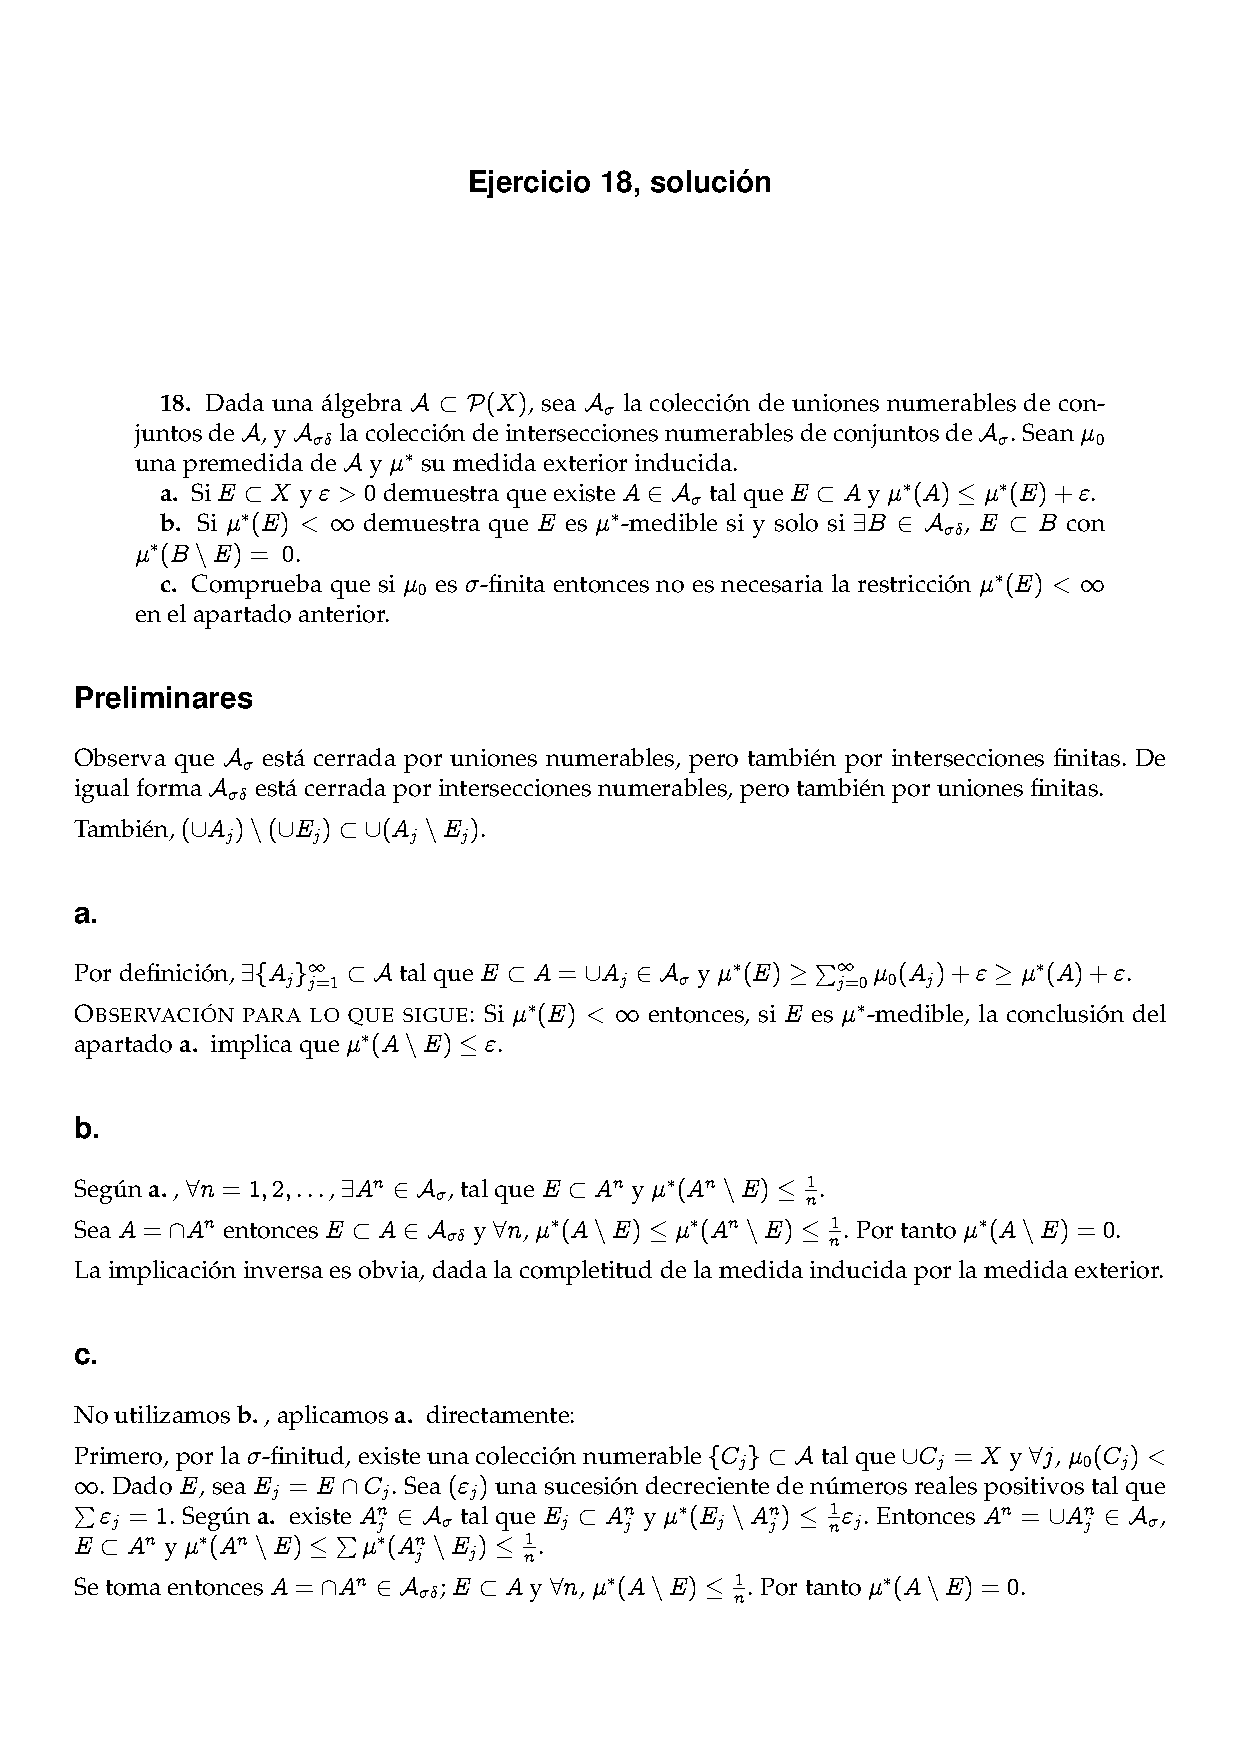
\includepdf[scale=0.9]{pdf/2014-03-18.pdf}
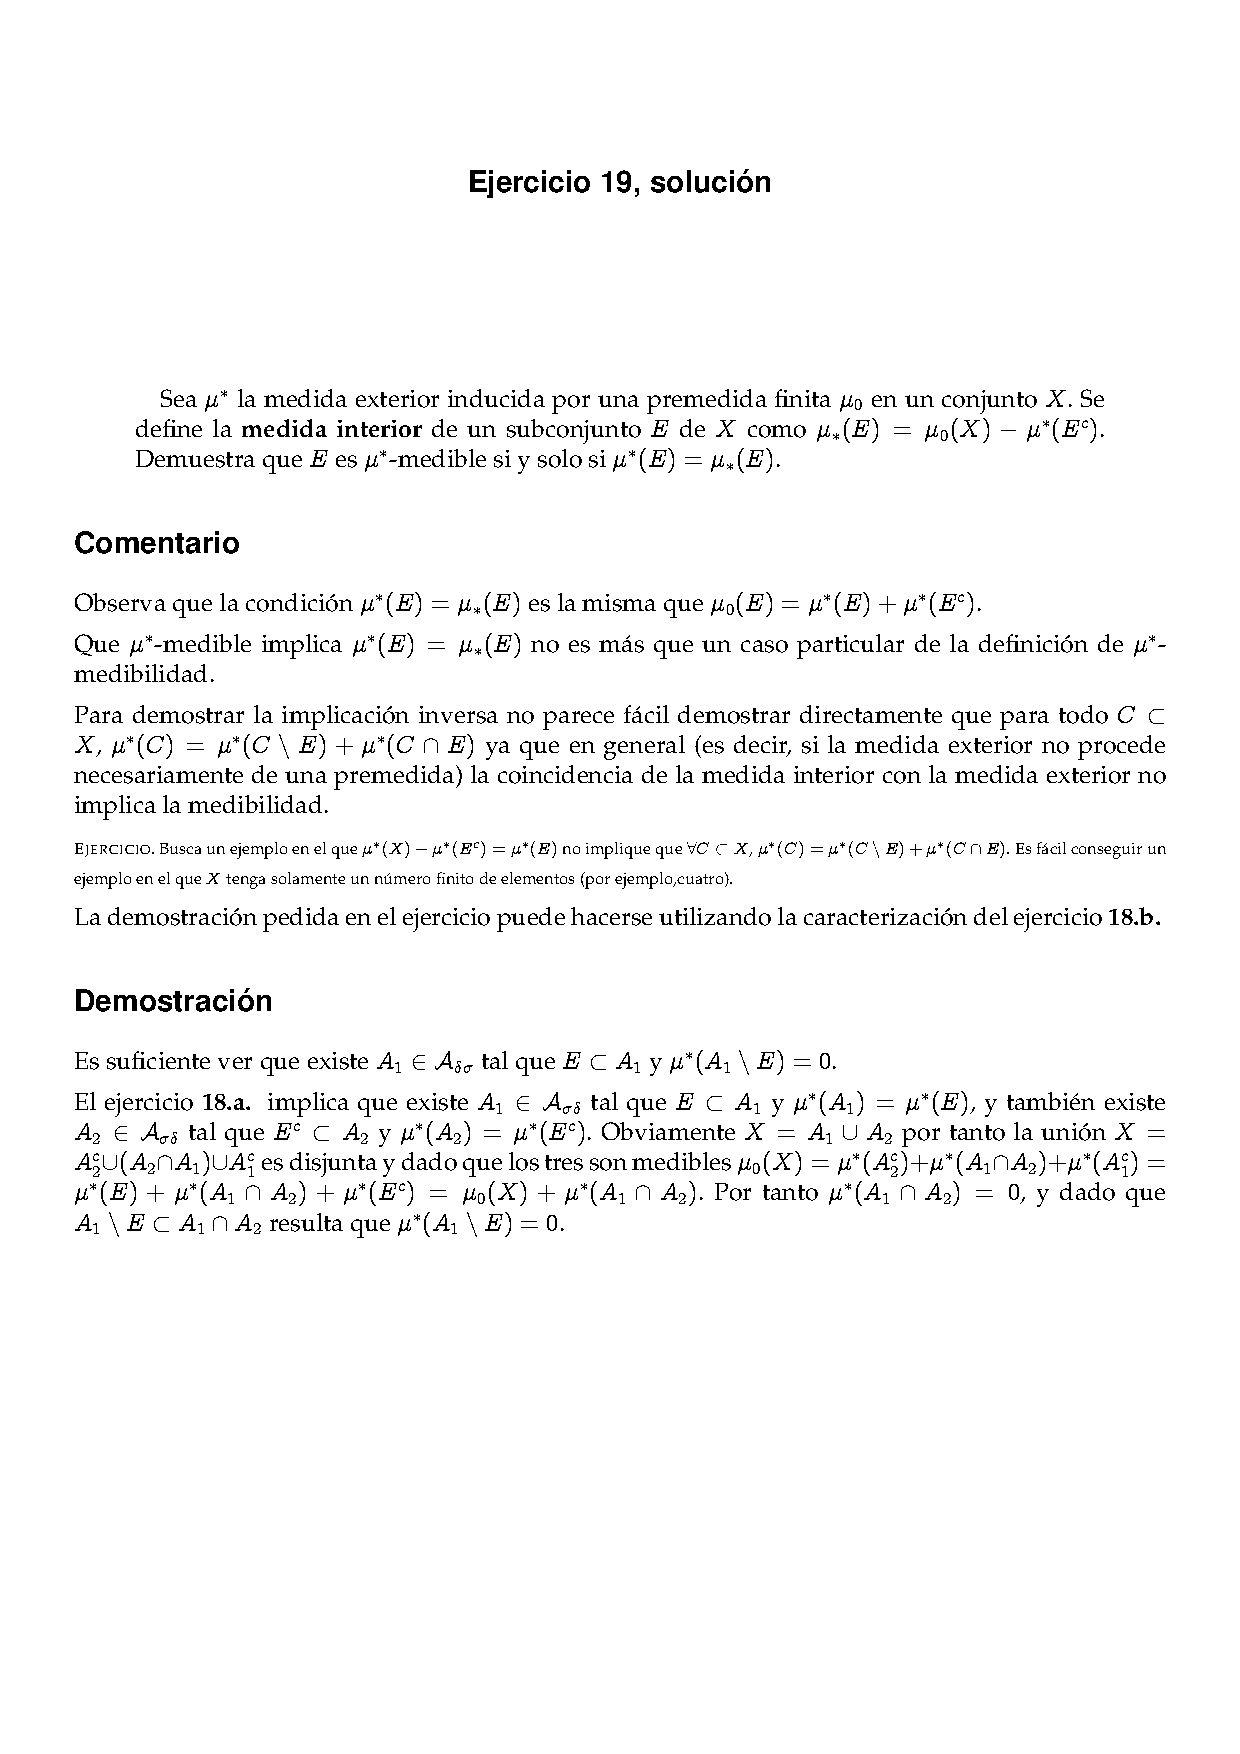
\includepdf[scale=0.9]{pdf/2014-03-19.pdf}
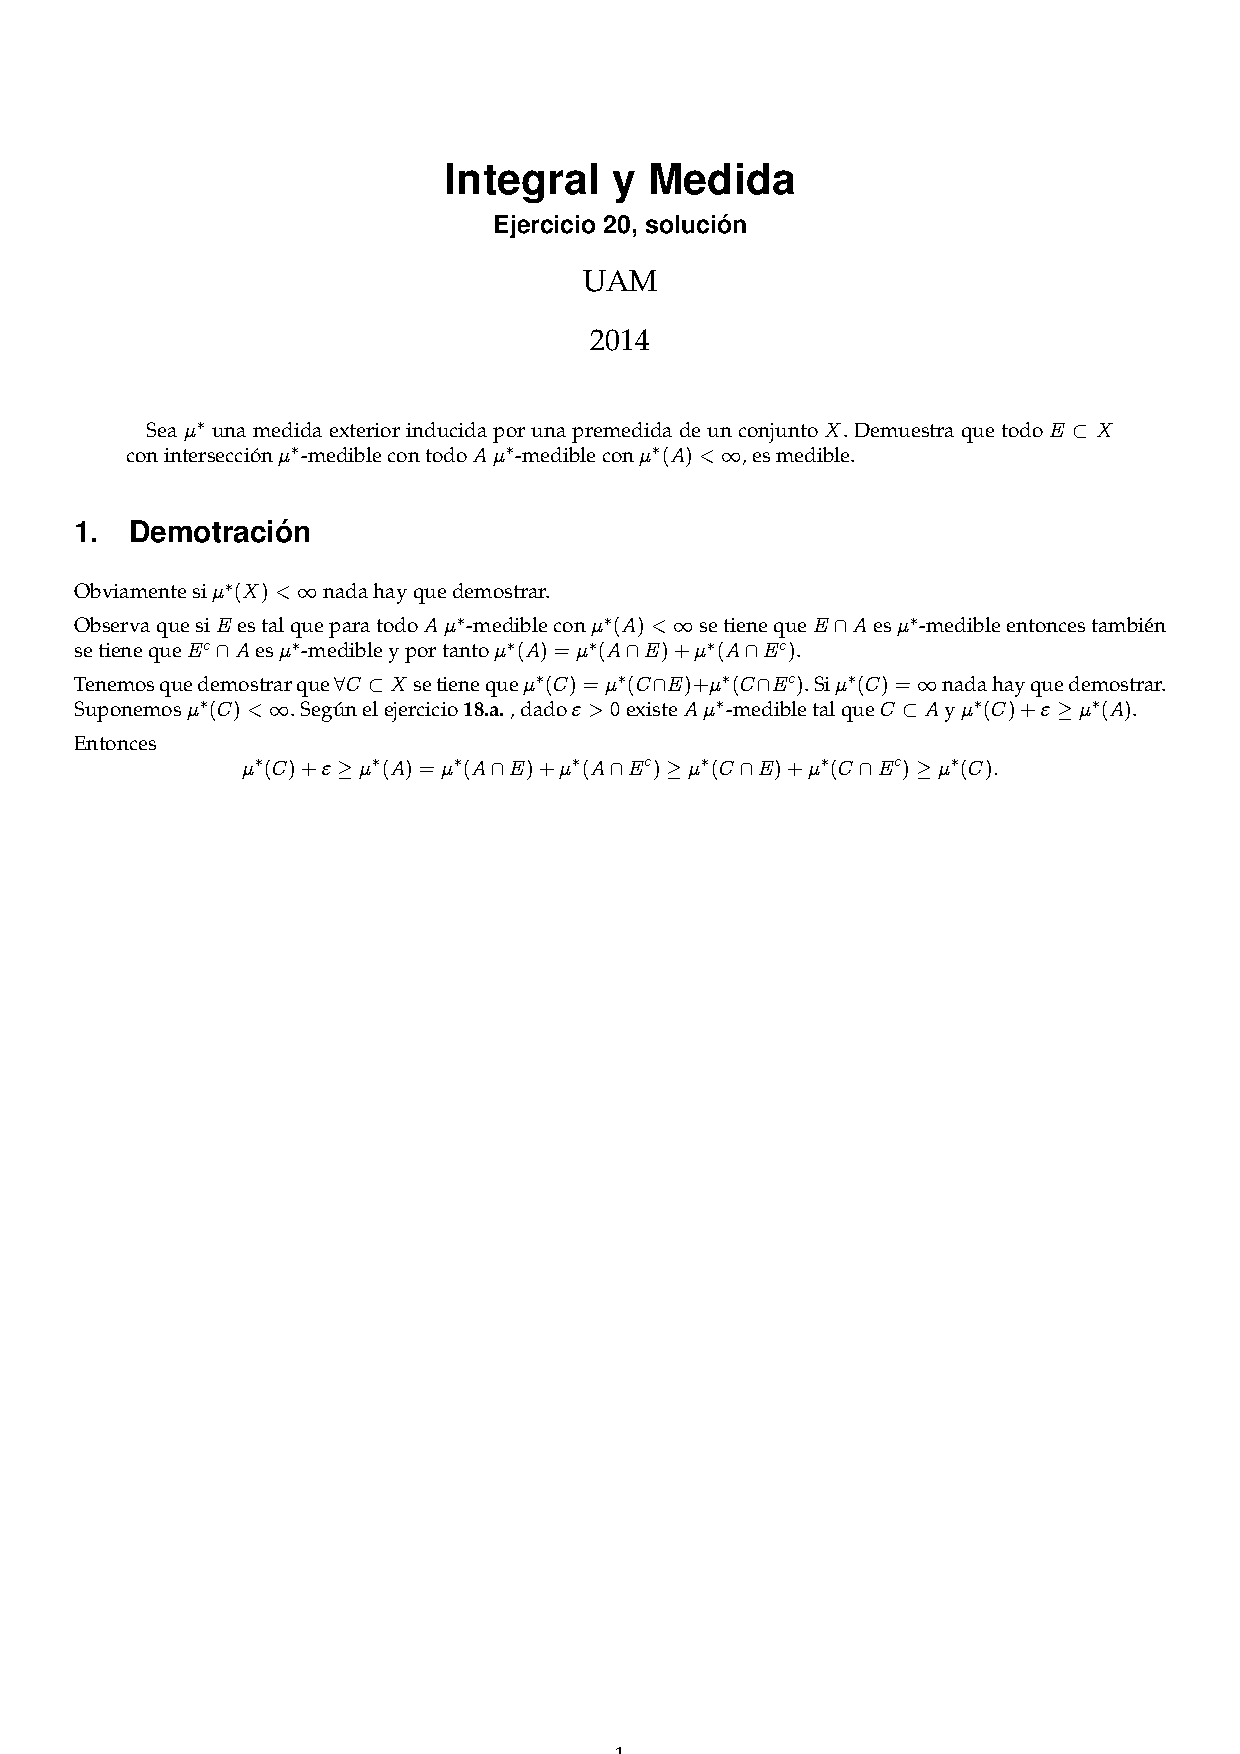
\includepdf[scale=0.9]{pdf/2014-03-20.pdf}

\subsection{Hoja 4}

\begin{problem}
Sea µ la medida de Lebesgue-Stieltjes asociada a la función:
\[F(x)=\left\{ \begin{array}{lcc}
             0 &   \text{si}  & x < 1 \\
             \\ x & \text{si} & 1 \leq x < 3 \\
             \\ 4 &  \text{si}  & 3 \leq x
             \end{array}
   \right.\]

Calcula las siguientes medidas:
\solution
\begin{itemize}
\item $µ(\{1\}) = F(1)-\displaystyle\lim_{x \to 1^-} F(x)$ = 1
\item $µ(\{2\}) = 0$
\item $µ((1, 3]) = F(3)-F(1) = 4 - 1 = 3$
\item $µ((1, 3)) = µ((1, 3]) - µ(\{3\}) = 3 - 1 = 2$
\item $µ([1, 3)) = µ((1, 3)) + µ(\{1\}) = 2 + 1 = 3$
\item $µ([1, 3])) = µ((1, 3]) + µ (\{1\}) = 3 + 1 = 4$
\end{itemize}
\end{problem}

\begin{problem}
Halla funciones de distribución $F$, $F_1$, $F_2$ de forma que, en cada caso, existan $a$ y $b$ tales que:
\begin{enumerate}
\item $µ((a,b)) < F(b)-F(a) < µ([a,b])$, donde $µ=µ_F$
\item $µ_1((a,b)) < µ_1((a,b]) < µ_1([a,b)) < µ_1([a,b])$ y

$µ_2((a,b)) < µ_2([a,b)) < µ_2((a,b]) < µ_2([a,b])$ donde $µ_i = µ_F, \ i=1,2$
\end{enumerate}
\solution
\begin{enumerate}
\item Vale con la función del ejercicio anterior
\item
\textbf{Con i = 1}
\[F_1(x)=\left\{ \begin{array}{lcc}
             0 &   si  & x < 1 \\
             \\ x & si & 1 \leq x < 3 \\
             \\ 3.5 &  si  & 3 \leq x
             \end{array}
   \right.\]

\textbf{Con i = 2}
\[F_2(x)=\left\{ \begin{array}{lcc}
             0 &   si  & x < 1 \\
             \\ x & si & 1 \leq x < 3 \\
             \\ 5 &  si  & 3 \leq x
             \end{array}
   \right.\]
\end{enumerate}

La construcción de estas funciones se ha realizado por la cuenta de la vieja. Si repetimos los cálculos del ejercicio anterior con estas funciones podemos ver que se cumplen las condiciones pedidas (Incluso puede que entendamos de qué va esto)
\end{problem}

\begin{problem}
Sea µ la medida de contar en $(\real, \algbP(\real))$. Para un conjunto finito A $\subset \real$ se define $µ_A(B) = µ(B \cap A)$ para todo $B \subset \real$

\ppart Sea $A=\{1,2,...,n,...\}$ ¿Es $µ_A$ una medida de Lebesgue-Stieltjes?. En caso afirmativo halla $F$ tal que $µ_A=µ_F$
\ppart Sea $A=\{\frac{1}{1},\frac{1}{2},...,\frac{1}{n},...\}$ ¿Es $µ_A$ una medida de Lebesgue-Stieltjes?. En caso afirmativo halla $F$ tal que $µ_A=µ_F$
\solution


\spart Esta medida simplemente cuenta el número de enteros positivos que hay en un conjunto $B$.

Por tanto, simplemente tenemos que buscar una función que realice esa misma función, por ejemplo:
\[F(x)=\left\{ \begin{array}{lcc}
             0 &   si  & 0 \leq x < 1 \\
             \\ n &  si  & n \leq x < n+1
             \end{array}
   \right.\]

Imitando las cuentas realizadas en el ejercicio 1 podemos que ver:
\begin{itemize}
\item $µ((1,3])) = F(3) - F(1) = 2$
\item $µ((1,3)) = µ((1,3])) - µ(\{3\}) = 2 - 1 = 1$
\end{itemize}
observamos que, efectivamente, obtenemos el número de enteros de cada intervalo.

\spart Esta medida cuenta el número de racionales de la forma $\frac{1}{n}$ que hay en un conjunto.

Esta medida no es de Lebesgue-Stieltjes. Una medida de Lebesgue-Stieltjes tiene que tener asociada una función $F$ como en el apartado anterior, es decir, tal que $μ((a,b]) = F(b) - F(a)$, y esta no puede tenerla.

Veamos por qué: tomemos el intervalo $B = (0,ε)$. Su medida según $μ_A$ es infinita, ya que para todo $n$ mayor que $\frac{1}{ε}$, $\frac{1}{n} ∈ A$, y entonces $B∩A$ es infinito. Luego tenemos que encontrar un $F$ tal que $F(ε) - F(0) = ∞$, y la única forma de que eso tenga sentido es que $F(ε) = ∞\; ∀ε$, lo cual es absurdo.

\end{problem}

\begin{problem}
Sea $F$ la función de distribución
\[F(x)=\left\{ \begin{array}{lcc}
             0 &   si  & x \in (-\infty, -1) \\
             \\ 1+x & si & x \in [-1, 0) \\
             \\ 2+x^2 & si & x \in [0, 2) \\
             \\ 9 &  si  & x \in [2, \infty)
             \end{array}
   \right.\]

Siendo $µ=µ_F$, hallar las siguientes medidas.
\solution
\begin{itemize}
\item $µ(\{2\}) = 3 $
\item $µ([-\frac{1}{2}, 3)) = 9 - \frac{1}{2}$
\item $µ((-1,0]\cup (1,2)) = 1 + µ((1,2]) - µ(\{2\}) = 1 + 9 -3 - 3 = 4$
\item $µ([0, \frac{1}{2}) \cup (1, 2]) = \frac{1}{4} + 6$
\item $µ(\{x \in \real \tq |x|+2x^2 > 1\})$=$µ((-\infty, -\frac{1}{2})) + µ((\frac{1}{2}, \infty)) = 0 + 9 - 2 - \frac{1}{4} = 7 - \frac{1}{4}$
\end{itemize}
\end{problem}

\begin{problem}
Sea $\appl{f}{\real}{\real}$ no negativa, integrable Riemann sobre cada intervalo finito y tal que $\int_{-\infty}^{\infty}f(x)=1$.

Prueba que $F(x)=\int_{-\infty}^x f(y) \dif y$ es una función de distribución de probabilidad y que, además, $F$ es continua ($f$ es la función de densidad de $F$).

Si $f(x)=\ind_{[0,1]}$ hallar $F$

\solution
Simplemente tenemos que ver que $F$ es no decreciente, continua por la derecha y que se cumple:
\[\lim_{n \to - \infty}F(x)=0 \ \ \lim_{n \to \infty}F(x)=1\]

Observando que $F$ es una integral y que integrar una función equivale a calcular el área encerrada bajo ella, vemos que a medida que avanzamos la $x$, cada vez estamos calculando un área mayor, luego los dos límites anteriores se cumplen.

Para ver que es continua por la derecha observamos que:
\[ \lim_{h \to 0^+}F(x+h) = \lim_{h \to 0^+} \int_{-\infty}^{x+h}f(y)\dif y = \int_{-\infty}^xf(y)\dif y = F(x)\]

Y es que por ser $F$ una integral, es obvio que es continua.

Suponemos ahora $f(x)=\ind_{[0,1]}$, para responder a la segunda pregunta del enunciado. Entonces
\[F(x)= \int_{-\infty}^{x} \ind_{[0,1]} = \left\{ \begin{array}{lcc}
             0 &   si  & x < 0 \\
             \\ x & si &  0 \leq x \leq 1 \\
             \\ 1 &  si  & 1 \leq x
             \end{array}
   \right.\]
\end{problem}

\begin{problem}
Halla el valor de $k$ para que $f= kx(1-x)\ind_{[0, 1)}$ sea la función de densidad de una medida de probabilidad. Calcula su función de distribución.

\solution
Para que sea función de densidad necesitamos que:
\[\int_{-\infty}^{\infty}f(x) dx = 1\]

Vamos a ver cuánto vale esa integral.
\begin{gather*}
\int_{-\infty}^{\infty}f(x) \dif x = \int_{-\infty}^{\infty}kx(1-x)\ind_{[0, 1)} \dif x  = \\
 = \int_{-\infty}^{0} kx(1-x)\cdot 0 \dif x + \int_{0}^{1}kx(1-x)\dif x + \int_{1}^{\infty}kx(1-x)\cdot 0 \dif x = \\
= k\left(\frac{1}{2}-\frac{1}{3}\right)
\end{gather*}


De donde obtenemos fácilmente que $k = \frac{1}{\frac{1}{2}-\frac{1}{3}} = 6$

La función de distribución sería:
\[\F(x)= \int_{-\infty}^{x} \ind_{[0,1]} = \left\{ \begin{array}{lcc}
             0 &   si  & x < 0 \\
             \\ \int_{0}^{x}kt(1-t)\dif t = (3x^2-2)x^3)& si &  0 \leq x \leq 1 \\
             \\ 1 &  si  & 1 \leq x
             \end{array}
   \right.\]
\end{problem}

\newpage
\begin{problem}
Dado $k$ > 0, sea $f(x)=αe^{-kx}\ind_{[0, \infty)}(x)$
\begin{enumerate}
\item Halla α para que $f$ sea una función de densidad de probabilidad
\item Sea $X$ una variable aleatoria con función de densidad f, si $k=\frac{1}{2}$, calcula la probabilidad de que $X \geq 3$
\item Si $k=\frac{1}{2}$ calcula la probabilidad de que $3 \leq X \leq 6$
\end{enumerate}
\solution
\begin{enumerate}
\item Repitiendo el proceso del ejercicio anterior, debemos hacer que $\int_{0}^{\infty}f(x)dx =1$.

En este caso obtenemos que α=k, es decir, nos encontramos ante una exponencial.

\item
\[\mathbb{P}(X \geq 3) = \int_{³}^{\infty}e^{-kx}dx=e^{\frac{3}{2}}\]

\item Puesto que la función de distribución es continua, la probabilidad de que $X=3$ ó $X=6$ es 0, de modo que podemos calcular la probabilidad pedida como:
\[\mathbb{P}(3 \leq X \leq 6) = \int_{3}^{6}e^{-kx}dx\]
\end{enumerate}
\end{problem}

\begin{problem}
Sea µ la medida de probabilidad definida por la función de distribución:

\[F(x)= \int_{-\infty}^{x} \ind_{[0,1]} = \left\{ \begin{array}{lcc}
             0 &   si  & x \in (- \infty, -1) \\
             \\ \frac{1}{3} & si &  x \in [-1, \sqrt{2}) \\
             \\ \frac{1}{2} + \frac{x-\sqrt{2}}{10} & si &  x \in [\sqrt{2}, 5) \\
             \\ 1 &  si  & x \in [5, \infty)
             \end{array}
   \right.\]

Calcular las siguientes medidas:
\solution

Antes de nada deberíamos comprobar que la función $F(x)$ dada es, efectivamente, una función de distribución. Para ello debemos comprobar que siempre es positiva y que se trata de una función creciente.

En este caso nos fiamos y se deja como ejercicio para el lector desconfiado (Edu) la comprobación de estas propiedades.
\newpage
\begin{enumerate}
\item \[µ((\real \setminus \rac)\cap[\sqrt{2}, 5]) = µ([\sqrt{2}, 5)) = µ((\sqrt{2}, 5]) + µ (\{\sqrt{2}\}) - µ (\{\sqrt{5}\}) =\]
\[ = F(5) - F(\sqrt{2}) +(\frac{1}{2}-\frac{1}{3}) -(1-(1-\frac{\sqrt{2}}{10}))=1-\frac{1}{2}+\frac{1}{6}-\frac{\sqrt{2}}{10}\]

\item \[µ((\real \setminus \rac)\cap [-2, \sqrt{2}]) = µ(\{\sqrt{2}\}) = \frac{1}{2}-\frac{1}{3} = \frac{1}{6}\]

\item \[µ(\rac \cap [1,6]) = µ(\{5\}) = \frac{\sqrt{2}}{10}\]
\end{enumerate}

Vamos ahora a por la parte complicada del ejercicio.

\[A_{3n-2} = \left(\frac{2n}{4n+3}, \frac{4n+5}{3n}\right)\]
\[A_{3n} = \left(\frac{4}{5n+2}, \frac{6n+1}{2n}\right)\]
\[A_{3n-1} = \left(-2, \frac{6n-1}{5n+2}\right)\]

Vemos que:
\begin{enumerate}
	\item $\lim A_{3n-2}= [\frac{1}{2}, \frac{4}{3}]$
	\item $\lim A_n{3n-1} = (-2, \frac{6}{5})$
	\item $\lim A_{3n} = (0^+, 3^+)$
\end{enumerate}

Recordemos que el límite superior de $A_n$ es el conjunto de puntos que están en infinitos conjuntos de la sucesión. Por tanto, todos los puntos contenidos en estos límites se contienen en el límite superior de la sucesión.
\[\limsup A_n = [\frac{1}{2}, \frac{4}{3}] \bigcup  (-2, \frac{6}{5}) \bigcup (0^+, 3^+)\]

Por otro lado, el límite inferior es el conjunto de puntos que se encuentran en todos los elementos de la sucesión a partir de uno dado. Así, el límite inferior será la intersección de los límites calculados anteriormente.
\[\liminf A_n = [\frac{1}{2}, \frac{4}{3}] \bigcap  (-2, \frac{6}{5}) \bigcap (0^+, 3^+)\]

\textcolor{blue}{Completado por mi. No fiarse al 100\%}
\[µ(\limsup A_n) = µ([\frac{1}{2}, \frac{4}{3}]) +  µ((-2, \frac{6}{5})) +µ((0^+, 3^+)) = \frac{1}{3}  + \frac{1}{3} + \frac{1}{3} = 1\]
\[µ(\liminf A_n) = µ([\frac{1}{2}, \frac{6}{5})) = 0\]

\end{problem}

\begin{problem}
Sea $\appl{F}{\real}{\real}$ una función de distribución
\begin{enumerate}
\item Prueba que el conjunto de puntos de discontinuidad de $F$ es numerable
\item Prueba que el conjunto de puntos de continuidad de $F$ es denso en $\real$
\end{enumerate}
\obs $F$ es monótona luego no tiene más discontinuidades que saltos
\solution

\begin{enumerate}
\item Vamos a probar que el número de puntos de discontinuidad en (n, n+1] es numerable.

Para ello tomamos la medida de este intervalo:
\[M = F(n+1)-F(n)\]

La pregunta que nos hacemos ahora es, ¿cuántos puntos $x \in (n, n+1]$ pueden tener $µ_F(\{x\}) \frac{M}{k}$?

La respuesta es sencilla (la supo hasta Elena en clase). $\forall k \in \nat$ No podemos tener más de k puntos con esta condición.

Por tanto no puede haber una cantidad no numerable de puntos de (n, n+1] con $µ_F(\{x\})>0$
%\item Si tuviésemos una cantidad no numerable de discontinuidades tendríamos un intervalo cerrado que contiene una cantidad no numerable de discontinuidades. Puesto que cada una de esas discontinuidades tenemos un salto, resulta que tendríamos un número no numerable de saltos en un intervalo cerrado.

%Así, tendríamos que la medida del intervalo cerrado sería la suma infinita y no numerable de valores positivos, lo que nos daría un resultado finito.

%Leyendo de un artículo de wikipedia:
%\begin{verbatim}
%La suma de los saltos no puede ser mayor que la diferencia de los
%valores de la función en los extremos del intervalo, de modo que
%el conjunto de discontinuidades con salto mayor que 1/n es finito
%y, por tanto, el conjunto de discontinuidades es a lo más numerable
%\end{verbatim}

\item \textcolor{blue}{Hecho por mi. No fiarse al 100\%}

Recordando lo dado en topología, sabemos que un conjunto es denso si la adherencia del conjunto coincide con el total.

Recordamos también que la adeherencia son aquellos puntos tales que todo abierto que lo contenta corta al conjunto dado.

Puesto que las únicas discontinuidades que puede presentar una función de distribución son discontinuidades de salto y es obvio que para cualquier punto en que la función sea continua todo entorno del punto contiene otros puntos de discontinuidad.
\end{enumerate}
\end{problem}

\begin{problem}
Variando si es necesario en cada caso el tamaño de los intervalos, construir un conjunto de tipo Cantor cuya medida de Lebesgue sea mayor que 1-ε
\solution
La construcción del conjunto de Cantor consiste en tomar el intervalo [0,1] y los siguientes conjuntos:
\begin{enumerate}
\item Construimos un intervalo $A_1$ de longitud $\frac{ε}{2}$ centrado en el intervalo [0,1].
\item Construimos $A_2 = \bigcup (a_i, b_i)$ tales que cada elemento de la unión tiene longitud igual a $\frac{1}{2}\frac{ε}{4}$.
\item etc
\end{enumerate}
Así, en el paso n-ésimo tenemos:
\[A_n = (a_1^n,b_1^n) \cup (a_2^n,b_2^n) \cup ... \cup (a_n^n,b_n^n)\]
donde cada intervalo de la unión tiene longitud $\frac{1}{2^{n-1}}\frac{ε}{2}$.

El conjunto de Cantor se obtiene restando del intervalo incial todos los intervalos $A_n$ que hemos ido construyendo. Es decir:
\[C = I -\bigcup A_n\]
\[m(C)=m(I)-\sum m(A_n) = 1 - ε\]
\end{problem}

\begin{problem}
Sea $µ_F$ la medida de Lebesgue-Stieltjes correspondiente a una función creciente y continua $\appl{F}{\real}{\real}$
\begin{enumerate}
\item Prueba que si A es numerable entonces $µ_F(A)$=0
\item Prueba que existen conjuntos A tales que $µ_F(A)> 0$ y A no contiene ningún intervalo abierto.
\item Si $µ(A)\geq 0$ y $µ(\real \setminus A) = 0$, ¿tiene que ser A denso en $\real$
\end{enumerate}
\obs Se recomienda construir una función $F(x)$ que sea constante en un intervalo
\solution

\begin{enumerate}
\item \textcolor{blue}{Hecho por mi. No fiarse al 100\%}

Si $A$ es numerable podemos escribirlo de la forma:
\[A = \bigcup_{i=1}^{\infty}\{a_i\} \tq a_i \neq a_j \forall i, j \ i \neq j\]
por tanto,
\[µ(A) = \sum_{i=1}^{\infty} µ(\{a_i\}) \]
pero, puesto que la función del enunciado es continua, la medida de un único punto siempre es 0 y por lo que
\[µ(A) = \sum_{i=1}^{\infty} µ(\{a_i\}) = \sum_{i=1}^{\infty}  0 = 0\]

\item Podemos tomar el conjunto $(a, b]$ que tendrá
\[µ((a,b]) = F(b)-F(a) \geq 0\]
ya que $F$ es creciente.

Ahora debemos cuida que no contenta abiertos. Para ello basta con tomar la intersección de este intervalo con los racionales.

Con ello eliminamos la posibilidad de que haya abiertos contenidos en el conjunto y mantenemos la medida del conjunto puesto que la medida de los racionales (que son los que estamos extrayendo) es 0.

\item No tiene por qué ser A denso. Pongamos un contraejemplo para probarlo.

Si tomo una función que crece entre el 0 y el 1 y luego se queda constante y tomo $A=(0,1)$ tenemos que se cumplen las condiciones del enunciado pero obviamente el intervalo $(0,1)$ en $\real$ no es denso.
\end{enumerate}
\end{problem}

\begin{problem}
Sea $F(x)=log(1 + |x|)\cdot \ind_{[0, \infty)}(x)$
\begin{enumerate}
\item Comprueba que $\appl{F}{\real}{\real}$ es creciente y continua por la derecha.
\item Calcula $µ_F(\{Cantor\})$
\end{enumerate}
\obs El conjunto de Cantor está contenido en $2^n$ intervalos de longitud $\frac{1}{3^n}$
\solution

\begin{enumerate}
\item \textcolor{blue}{Hecho por mi. No fiarse al 100\%}

Tenemos que ver que $a<b \implies F(a) < F(b)$ lo cual es obvio ya que el logaritmo es creciente y la función indicatriz simplemente vale 0 cuando $x4 < 0$ y 1 en el resto de casos.

Para ver que es contínua por la derecha necesitamos probar que:
\[\lim_{x \to a^+}F(x) = F(a) \ \forall a \in X\]
El único punto donde podemos dudar es en $a=0$ pero en ese caso está claro que:
\[\lim_{x \to 0^+}F(x) = \log(1) = 0 = F(0)\]

\item
\begin{defn}[Conjunto de Cantor]
Es el conjunto de todos los puntos del intervalo real [0,1] que admiten una expresión en base 3 que no utilice el dígito 1
\end{defn}

\[µ_F(\{Cantor\}) = 1 - \frac{1}{3}+2\frac{1}{9}+4\frac{1}{27}+... = \frac{1}{3} \sum_{n=1}^{\infty}\left(\frac{2}{3}\right)^{n-1} = \frac{1}{3} \frac{1}{1-\frac{2}{3}} = 1-1 = 0\]

\end{enumerate}
\end{problem}

\begin{problem}
Sea µ una medida de Borel en $\real$, finita sobre compactos, con $µ((0, 1])=1$
\begin{enumerate}
\item Prueba que si $\forall s \in \real, µ(s + E)=µ(E)$, entonces µ es la medida de Lebesgue.
\item Prueba que si $\forall s \in \real, µ(rE)=|r|µ(E)$, entonces µ es la medida de Lebesgue
\end{enumerate}
\solution
\begin{enumerate}
\item
Para ver que es la medida de Lebesgue necesitamos ver que
\[\forall a,b \ a<b \ µ((a,b]) = b-a\]
Por continuidad podemos restringirnos a trabajar con a,b racionales.

Por la invarianza por traslaciones es suficiente ver:
\[\forall b \in \rac \ µ((0,b])=b\]

Vamos a ello pues
\[µ((0, \frac{p}{q}]) = \sum_{i=1}^{\infty} µ((\frac{1-i}{q}, \frac{i}{q}]) = p\cdot µ((0, \frac{1}{q}])\]

Ahora sólo nos queda ver que $µ((0, \frac{1}{q}]) = \frac{1}{q}$, pero para ello basta con fijarnos en que:
\[µ((0, 1]) = \sum_{i=1}^{\infty} µ((\frac{i-1}{q}, \frac{i}{q}]) = q \cdot µ((0, \frac{1}{q}])\]

\item Se hace prácticamente igual que el apartado anterior. Se deja como ejercicio para casa.


\end{enumerate}
\end{problem}

\begin{problem}
Sea µ la medida de Lebesgue de $\real$ y $E \subset \real$ medible Lebesgue tal que 0 < µ(E) < $\infty$. Demuestra que para todo α, 0<α<1, existe un intervalo abierto I tal que µ($I \cap E$) > α m(I)
\solution
Sabemos que la medida de Lebesgue se puede aproximar bien por abiertos que contengan al conjunto $E$, es decir:
\[\forall ε > 0 \ \exists A \text{ abierto con } E \subset A \tq µ(E) > µ(A)-ε \]

Tomamos $A= \bigcup_{k=1}^{\infty} I_k$ con los $I_k$ disjuntos.

Suponemos ahora que $\exists α \in (0,1) \tq \forall I \text{ intervalo abierto } µ(E \cap I)\leq αµ(I)$
Entonces
\[µ(E) = \sum_{k=1}^{\infty}µ(E \cap I_k) \leq \sum_{k=1}^{\infty} α µ(I_k) = α µ(A)\]

Si la suposición fuese cierta tendríamos ahora
\[µ(A)-µ(E) \geq µ(A) - α µ(A) (1-α)µ(A) \geq (1-α)µ(E) > ε\]
y llegamos a contradicción.
\end{problem}


\chapter{Ejercicios 1ª Hoja}
\section{Ejercicios sobre autómatas finitos y lenguajes regulares}

\begin{problem}[1]
Diseña expresiones regulares para los siguientes lenguajes:
\ppart$L(A) = \lbrace a^nb^m : \ n+m$ es impar $\rbrace$

\ppart Conjunto de números binarios que contienen la subcadena 1010

\ppart Identificadores de un lenguaje de programación que empiezan con el símbolo @, seguido de una letra minúscula y cualquier combinación de letras minúsculas o números.

\solution

\spart
$(aa)*.(a+b).(bb)*$

\spart
$(1+0)*.1010.(1+0)*$

\spart
$@.(a+b+...+z).(0+1+...+9+a+b+...+z)*$
 

\end{problem}


\begin{problem}[2]
Diseña un autómata finito (determinista o no determinista) que reconozca cada uno de los siguientes lenguajes:
\ppart Conjunto de números binarios que contienen la subcadena 1010

\ppart Identificadores de un lenguaje de programación que empiezan con el símbolo @, seguido de una letra minúscula y cualquier combinación de letras minúsculas o números.

\solution
Escojo hacer los diagramas deterministas:\\
\spart
\begin{center}
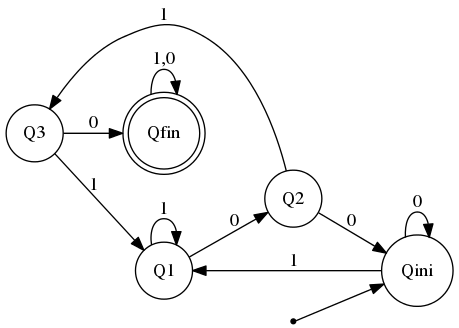
\includegraphics[scale=0.75]{tex/ejerciciosHoja1/automata_2a.png}
\end{center}

\spart
 Las transiciones no indicadas sobreentendemos que van a un nodo residuo.

\begin{center}
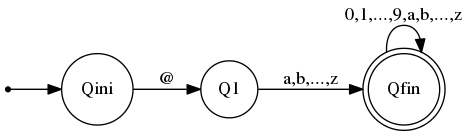
\includegraphics[scale=0.75]{tex/ejerciciosHoja1/automata_2b.png}
\end{center}

 

\end{problem}


\begin{problem}[3]
Indica cuál es el lenguaje aceptado por el siguiente autómata:\\
\begin{center}
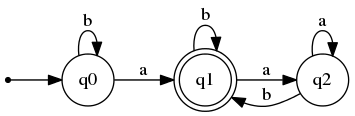
\includegraphics[scale=0.75]{tex/ejerciciosHoja1/automata_3.png}
\end{center}


\solution
Expresión regular: $L(A)=b^*.a+b^*.a.(a+b)^*.b$

Aunque nos pida el lenguaje nos vale con poner la expresión regular.


\end{problem}


\begin{problem}[4]
Construye un autómata finito determinista que acepte cadenas sobre el alfabeto {0,1} que representen números enteros y múltiplos de 5 expresados en representación binaria.

\solution
\begin{expla}
Los estados representan el resto de dividir el número entre 5. Se tiene en cuenta que si tienes un numero cualquiera (por ejemplo 101) al añadirle un 0, es como multiplicarlo por 2, por tanto su resto es el doble, y al añadirle un 1, es como multiplicarle por 2 y sumarle 1.
\end{expla}
\begin{center}
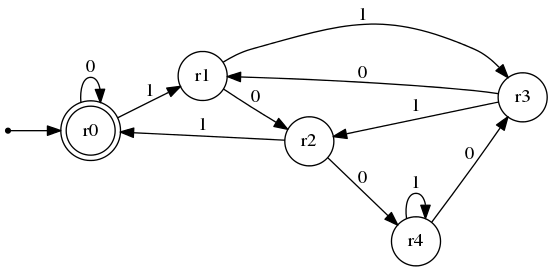
\includegraphics[scale=0.75]{tex/ejerciciosHoja1/automata_4.png}
\end{center}

\end{problem}

 
 \begin{problem}[5]
 Para el autómata siguiente encuentra $\delta^*(q_0,1011)$ y $\delta^*(q_1,01)$ 
 \begin{center}
 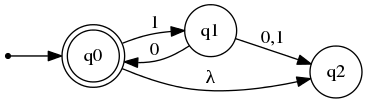
\includegraphics[scale=0.75]{tex/ejerciciosHoja1/automata_5.png}
 \end{center}
 
 \solution
 \begin{expla}
 Nos piden la salida del autómata dada un estado inicial y una palabra.
 \end{expla}
 

 $\delta^*(q_0,1011)$ = q2 \\
 \begin{tabbing}
   \hspace*{2cm} \= \hspace*{2cm} \= \hspace*{2cm} \= \hspace*{2cm} \= \hspace*{2cm} \kill
 Estados \> 1   \> 0   \> 1   \> 1  \\
 q0 \> q1 \> q0 \> q1\> q2  \\
  \>  \> q2 \> - \> -\\
 q2 \> - \> - \> - \> -\\
 \end{tabbing}
 

 $\delta^*(q_1,01)$ = $q1$ \\
  \begin{tabbing}
  \hspace*{2cm} \= \hspace*{2cm} \= \hspace*{2cm} \kill
  Estados \> 0   \> 1  \\
  q1 \> q0 \> q1 \\
   \> q2 \> -\\
  \end{tabbing}
  
 
 \end{problem}
 
 
 \begin{problem}[6]
 Construye un autómata finito no determinista con tres estados que acepte el lenguaje $L=\{ab,abc\}^*$, ¿es posible hacerlo con menos de tres estados?
 
 \solution
 \begin{center}
 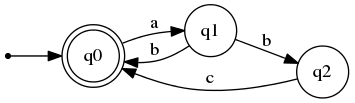
\includegraphics[scale=0.75]{tex/ejerciciosHoja1/automata_6.png}
 \end{center}
  
 
 \end{problem}
 
 \newpage

 
 
 
 
 \section{Ejercicios sobre autómatas a pila y gramáticas independientes del contexto}
 
 \begin{problem}[1]
 Diseña una gramática independiente del contexto que genere el lenguaje de los números capicúa formados con el alfabeto $\Sigma = {0,1,2,3,4,5,6,7,8,9} $. Los números de una sola cifra no se consideran capicúa.
 

 \solution
 
 
  En cada regla, si aparecen dos 'X' estas tienen que acabar en el mismo símbolo terminal. La otra opción era poner muchas reglas más tipo $X_0,...,X_9$.
  
  $S \longrightarrow XZX$
  
  $Z \longrightarrow XZX|X|\lambda$
  
  $X\longrightarrow 0|1|2|3|4|5|6|7|8|9$
 
 \end{problem}
 
 \begin{problem}[2]
 Diseña una gramática independiente del contexto que genere el lenguaje de los números formados con el alfabeto $\Sigma = {0,1,2,3,4,5,6,7,8,9} $ que tengan el mismo número de dígitos pares e impares. Puede suponer por simplicidad que los números pueden tener ceros a la izquierda.
 
 
 \solution
 $S \longrightarrow PSI|ISP|PI|IP|SS$
 
  $P \longrightarrow 0|2|4|6|8$
  
  $I \longrightarrow 1|3|5|7|9$
  
  
 
 \end{problem}
 
 \begin{problem}[3]
Diseña un autómata a piña que reconozca el lenguaje del ejercicio 1.
 
 
 \solution
 \begin{expla}
 Cuando pongo 'x' o 'y' quiero decir un símbolo del conjunto \{0,1,2,3,4,5,6,7,8,9\}. Cuando pongo 'x' e 'y' en la misma transición, $x \neq y$.
 \end{expla}
 \begin{center}
  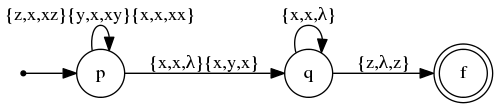
\includegraphics[scale=0.75]{tex/ejerciciosHoja1/automata_7.png}
  \end{center}
 
 \end{problem}
 
 \begin{problem}[4]
 Demuestra que la siguiente gramática es ambigua:
 
 $S \longrightarrow AB | aaB$
 
 $A \longrightarrow a|Aa$
 
 $B\longrightarrow b$
 
 
 \solution
 Si derivamos usando la primera regla de S obtenemos:\\
 $S \longrightarrow AB \longrightarrow AaB \longrightarrow aaB \longrightarrow aab $
 
  Si derivamos usando la segunda regla de S obtenemos:\\
  $S \longrightarrow aaB \longrightarrow aab$
 
 \end{problem}
  
  \begin{problem}[5]
  Encuentra una gramática independiente del contexto para el siguiente lenguaje:\\
  $L=\{a^nww^Rb^n:w\in\{a,b\}^*, n\geq1\}$
  
  \solution
  $w^R$, es la imagen simétrica de la cadena $w$. Si $w$ es $aab$, $w^R$ es $baa$.
  
   $S \longrightarrow aSb | aXb | $
   
   $X \longrightarrow aXa | bXb | \lambda$

  
  \end{problem}
  
  \begin{problem}[6]
  Indica cuál es el lenguaje aceptado por el siguiente autómata a pila:\\
  $A = (\{q_0,q_1,q_2\},\{a,b\},\{a,b,z\},\delta,q_0,z,\{q_2\})$\\
  $\delta(q_0,a,z) = \{(q_1,a),(q_2,\lambda)\} $\\
   $\delta(q_1,b,a) = \{(q_1,b)\} $\\
   $\delta(q_1,b,b) = \{(q_1,b)\} $\\
   $\delta(q_1,a,b) = \{(q_2,\lambda)\} $\\
  
  \solution
  El autómata a pila sería el siguiente:
  \begin{center}
    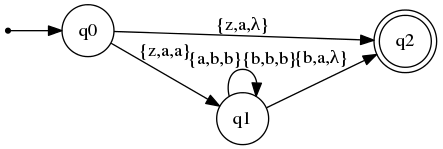
\includegraphics[scale=0.75]{tex/ejerciciosHoja1/automata_8.png}
   \end{center}
   El lenguaje consiste en expresiones del tipo $\{a\}\cup\{ab^n a\\forall n>0\}$
  
  \end{problem}
  
  
  
 
 
 
 
 
 
 
\end{document}


\chapter{Ejercicios 2ª Hoja}
\section{Ejercicios sobre Gramáticas de Atributos}
La gramática:
\begin{verbatim}
axioma         ::= USUARIO peliculas
peliculas      ::= peliculas peliculas | pelicula
pelicula       ::= TITULO valoraciones
valoraciones   ::= valoraciones valoracion valoracion
valoracion     ::= (USUARIO:NUMERO)
\end{verbatim}
genera frases que consisten en una secuencia de películas con sus respectivas valoraciones realizadas por los usuarios.Al principio de las frases generadas por la
gramática siempre aparece el nombre de un usuario. A continuación se muestran tres ejemplos:

jaime Star\_Wars(jaime:10)(ana:10) Spiderman(ana:10)(pepe:1)

ana Kapax(pepe:100)(jaime:1) Avatar(ana:40) Pi(pepe:100)(ana:1)

mike Kapax(pepe:100)(jaime:1) Avatar(ana:40) Pi(pepe:100)(ana:1)


Se desa añadir a esta gramática un sistema de atributos que haga lo siguiente:
\begin{enumerate}
\item Calcular el número total de películas valoradas
\item Indicar el título y la valoración de la película mejor valoradas por el usuario indicado al principio de la cadena. Si no hay ninguna películas valorada por dicho usuario debe indicarse tal circunstancia.
\end{enumerate}

Por ejemplo, para las tres cadenas anteriores se mostrarían respectivamente los mensajes siguientes:

Se han valorado 2 películas.
La mejor valorada por jaime es Star\_Wars, con una valoración de 10.

Se han valorado 3 películas.
La mejor valorada por ana es Avatar, con una valoración de 40.

Se han valorado 3 películas.
Ninguna película ha sido valorada por mike.


\textbf{Notas:}
\begin{itemize}
\item Puede considerarse que existe un proceso de análisis morfológio que asigna a los símbolos terminales los siguientes atributos semánticos: USUARIO.nombre (nombre de usuario), TITULO.titulo (título de la película), NUMERO.valor (valor numérico del número)
\item Debe comprobarse que el usuario que aparece al principio de la cadena no valora más de una vez la misma película. No es necesario realizar esta comprobación para el resto de usuarios.
\item No está permitido el uso de información global
\item Debe responderse a cada una de las cuestiones usando las plantillas correspondientes
\end{itemize}
\newpage

\begin{problem}[1]
Describa explícita y brevemente el significado de cada atributo que utilice, así como el proceso de actualización de cada uno de ellos mencionando si se realiza herencia o síntesis en su propagación. Responde rellenando la tabla:
\solution
\begin{tabular}{|c|c|l|}
\hline
SÍMBOLO & ATRIBUTOS & DESCRIPCIÓN \\
\hline
\hline
USUARIO & nombre & Nombre del usuario.\\
\hline
TITULO & titulo & Título de la película.\\
\hline
NÚMERO & valor & Valor numérico del número.\\
\hline
valoración & nota & nota de la valoración (por síntesis) \\
\cline{2-3}
& usuario & usuario que da la valoración (por síntesis)\\
\hline
valoraciones & usuario\_actual & Usuario inicial (por herencia)\\
\cline{2-3}
& notaMax & nota máxima (por síntesis) \\
\hline
& nota & Nota máxima de la película (por síntesis)\\
\cline{2-3}
película & titulo & titulo de la película (por síntesis) \\
\cline{2-3}
& usuario\_actual & Usuario inicial (por herencia) \\
\hline
& num & Número de películas valoradas (por síntesis)\\
\cline{2-3}
películas & usuario\_actual & Usuario inicial (por herencia) \\
\cline{2-3}
& titulo & titulo de la película mejor valorada (por síntesis) \\
\cline{2-3}
& nota & nota de la película mejor valorada (por síntesis)\\
\hline
\end{tabular}
\end{problem}

\begin{problem}[2]
Define formalmente la gramática utilizando la notación explicada en el temario de esta asignatura. Utiliza la siguiente tabla, en la que debes indicar, para cada regla de la gramática, las acciones semánticas asociadas junto con el instante en que se deben ejecutar.
\solution
\begin{tabular}{|c|l|}
\hline
INSTATE & ACCIÓN \\
\hline
\multicolumn{2}{|l|}{axioma ::= USUARIO peliculas} \\
\hline
 1 & peliculas.usuario\_actual = USUARIO.nombre \\
\hline
 2 & print("Se han valorado " + peliculas.num + " películas") \\
 & print("la mejor valorada por " + USUARIO.nombre + " es " + peliculas.titulo \\ & + " con una valoración de " + peliculas.nota + ".")\\
 \hline
\multicolumn{2}{|l|}{peliculas\_1 ::= peliculas\_2 pelicula} \\
\hline
 0 & peliculas\_2.usuario\_actual = peliculas\_1.usuario\_actual \\ & pelicula.usuario\_actual = peliculas\_1.usuario\_actual\\
 \hline
 2 & if(peliculas\_2.nota>pelicula.nota)\{\\ &
 peliculas\_1.nota=peliculas\_2.nota\\ &
 peliculas\_1.titulo=peliculas\_2.titulo\}\\ &
 else\{peliculas\_1.nota=pelicula.nota\\ &
 peliculas\_1.titulo=pelicula.titulo\}\\ &
 peliculas\_1.num = peliculas\_2.num+1\\
\hline
\multicolumn{2}{|l|}{peliculas ::= pelicula} \\
\hline
 0 & pelicula.usuario\_actual = peliculas.usuario\_actual \\
 \hline
 1 & peliculas.titulo = pelicula.titulo \\ & peliculas.nota = pelicula.nota \\ &
 peliculas.num=1\\
\hline
\multicolumn{2}{|l|}{pelicula ::= TITULO valoraciones} \\
\hline
0 & valoraciones.usuario\_actual = pelicula.usuario\_actual \\
 \hline
 1 & pelicula.titulo = TITULO.titulo \\
 \hline
 2 & pelicula.nota=valoraciones.notamax\\
\hline
\multicolumn{2}{|l|}{valoraciones\_1 ::= valoraciones\_2 valoracion} \\
\hline
0 & valoraciones\_2.usuario\_actual = valoraciones\_1.usuario\_actual\\
\hline
2 & if(valoraciones\_1.usuario\_actual==valoracion.usuario AND valoraciones\_2.notamax\\& $\neq$ 0)\{\\ &
print("ERROR")\\&
\}else if(valoraciones\_1.usuario\_actual==valoracion.usuario)\}\\&
valoraciones\_1.notamax=valoracion.nota\\&
\}else if(valoraciones\_2.notamax $\neq$0)\{\\&
valoracion\_1.notamax=valoraciones\_2.notamax\\&
\}else\{valoraciones\_1.notamax=0\}\\
\hline
\multicolumn{2}{|l|}{valoraciones ::= valoracion} \\
\hline
 0 & valoraciones.notamax=0 \\
 \hline
 1 & if(valoraciones.usuario\_actual==valoracion.usuario)\{\\ &
 valoraciones.notamax=valoracion.nota\}\\
\hline
\multicolumn{2}{|l|}{valoracion ::= (USUARIO:NUMERO)} \\
\hline
 2 & valoracion.nota = NUMERO.valor\\ & valoracion.usuario=USUARIO.nombre\\
 \hline

\end{tabular}

\end{problem}


\begin{problem}[4]
Considérese la siguiente gramática independiente del contexto:
\begin{verbatim}
axioma        ::= DINERO lista_compra
lista_compra  ::= compra lista_compra | compra
compra        ::= [PRODUCTO, PRECIO]
\end{verbatim}
Esta gramática genera sentencias que consisten en una cantidad de DINERO seguida de una lsita de compras, cada una con un PRODUCTO y el PRECIO del mismo. Tanto el DINERO como el PRECIO son números reales.

Se desa añadir a esta gramática un sistema de atributos que compruebe si se puede hacer la compra con el dinero disponible. Se indicarán los productos de la lista que se pueden comprar y el saldo disponible al final. Se supone que los productos se adquieren en el mismo orden en el que aparecen en la lista.

\textbf{Notas:}
\begin{itemize}
\item Puede considerarse que existe un proceso de análisis morfológico que asigna a los símbolos terminales los siguientes aributos semánticos: PRODUCTO.nombre (nombre del producto), PRECIO.valor (valor numérico del precio) y DINERO.valor (valor numérico del dinero).
\item No está permitido el uso de información global
\end{itemize}
\solution
Los atributos que debemos añadir son:
\begin{itemize}
\item \textbf{lista\_compra}
Añadimos los atributos: items, coste y saldo
\item \textbf{compra}
Añadimos los atributos: item y coste
\end{itemize}

La gramática de atributos resultante sería:
\begin{verbatim}
axioma          ::= DINERO lista_compra
{Herencia; lista_compra.saldo = DINERO}

lista_compra_1  ::= compra lista_compra_2
{Herencia;
    if lista_compra_1.saldo < compra.coste:
        lista_compra_2.saldo = lista_compra_1.saldo
    else
        lista_compra_1.saldo = lista_compra_2.saldo - compra.coste
        print compra}


lista_compra    ::= compra
{Herencia;
    if lista_compra.saldo >= compra.coste:
        print compra}

compra          ::= [PRODUCTO, PRECIO]
{compra.coste = PRODUCTO}
{Síntesis; compra.item = PRODUCTO}
\end{verbatim}
\end{problem}

\begin{problem}[5]
Considérese la siguiente gramática independiente del contexto:
\begin{verbatim}
romano ::= IList | I V | V IList
IList  ::= IList I | λ
\end{verbatim}
Esta gramática genera sentencias entre las que se encuentran los números romanos hasta el 8.

Se pide añadir a la gramática un sistema de atributos que compruebe si la sentencia corresponde a un número romano correcto y, en caso afirmativo, imprima su valor numérico.

\textbf{No está permitido el uso de información global}
\solution
\begin{verbatim}
romano ::= IList
{romano.esValido = IList.esValido}

romano ::= I V
{romano.esValido = true}

romano ::= V IList
{síntesis; romano.esValido = IList.esValido}

IList_1  ::= IList_2 I
{Síntesis; if IList_2.esValido & IList_2.items < 3 , IList_1.esValido = true}
{Síntesis; IList_1.items = IList_2.items + 1}

IList ::= λ
{IList.esValido = true}
{IList.items = 0}
\end{verbatim}
\end{problem}

\begin{problem}[6]
Considérese la gramática independiente del contexto resultante de añadir a la del ejercicio 5 el siguiente axioma:
\begin{verbatim}
S ::= romano = IList
\end{verbatim}
Esta gramática genera sentencias formadas por dos cadenas separadas por el signo '='. La primera cadena es igual que las generadas por la gramática del ejercicio 5. La segunda cadena es una lista de símbolos I.

Se pide añadir a la gramática un sistema de atributos que compruebe si, en el caso de que la primera cadena sea un número romano correcto, el valor del mismo coincide con el número de símbolos I en la segunda cadena.

\textbf{No está permitido el uso de información global}
\solution
\begin{verbatim}
S      ::= romano = IList
{Síntesis; if (romano.esValido & romano.value == IList.items), OK}

romano ::= IList
{Síntesis; romano.esValido = IList.esValido}
{Síntesis; if (IList.esValido), romano.value=IList.items}

romano ::= I V
{Síntesis; romano.esValido = true}
{Síntesis; romano.value = 4}

romano ::= V IList
{Síntesis; romano.esValido = IList.esValido}
{Síntesis; if (Ilist.esValido) romano.value = IList.items + 5}

IList_1  ::= IList_2 I
{Síntesis; if (IList_2.esValido & IList_2.items < 3) , IList_1.esValido = true}
{Síntesis; IList_1.items = IList_2.items + 1}

IList ::= λ
{IList.esValido = true}
{IList.items = 0}
\end{verbatim}
\end{problem}
\end{document}


\chapter{Ejercicios 3ª Hoja}
\section{Ejercicios de análisis}

%%%%%%%%%%%%%%%%%%%%%%%%%%%%%%%%%%%%%%%%%%%%%%%
%%%
%%% 		Problema 1
%%%
%%%%%%%%%%%%%%%%%%%%%%%%%%%%%%%%%%%%%%%%%%%%%%%
\begin{problem}
Sea la siguiente gramática:
\begin{itemize}
\item S ::= A
\item S ::= B
\item A ::= cA+b
\item A ::= a
\item B ::= cB+a
\item B :== b
\end{itemize}
 Calcula los conjuntos primero y siguiente para cada símbolo no terminal
\solution
\textbf{Primeros:}

\begin{itemize}
\item Primero(A) =$\{c,a\}$
\item Primero(B) =$\{c,b\}$
\item Primero(S) =$\{a,c,b\}$
\end{itemize}

\textbf{Sigueintes}

\begin{itemize}
\item siguiente(A) =$\{\$,+\}$
\item siguiente(B) =$\{\$, +\}$
\item siguiente(S) =$\{\$\}$
\end{itemize}
\end{problem}

%%%%%%%%%%%%%%%%%%%%%%%%%%%%%%%%%%%%%%%%%%%%%%%
%%%
%%% 		Problema 2
%%%
%%%%%%%%%%%%%%%%%%%%%%%%%%%%%%%%%%%%%%%%%%%%%%%
\begin{problem}
Sea la siguiente gramática LR(0):
\begin{itemize}
\item E ::= T
\item E ::= E + T
\item T ::= i
\item T ::= (E)
\end{itemize}
Calcula el cierre de la configuración inicial: E' ::= .ES
\solution
\begin{itemize}
\item E' ::= .ES
\item E ::= .T
\item E ::= .E + T
\item T ::= .i
\item T ::=.(E)
\end{itemize}
\end{problem}

%%%%%%%%%%%%%%%%%%%%%%%%%%%%%%%%%%%%%%%%%%%%%%%
%%%
%%% 		Problema 3
%%%
%%%%%%%%%%%%%%%%%%%%%%%%%%%%%%%%%%%%%%%%%%%%%%%
\begin{problem}
Sea la siguiente gramática LR(0):
\begin{itemize}
\item E ::= (L)
\item E ::= i
\item L ::= L,E
\item L ::= E
\end{itemize}

\ppart Calcula el cierre de la configuración E ::= (.L)

\ppart Calcula el estado al que se llega desde el estado anterior tras conocer el símbolo no terminal L.
\solution
\ppart
\begin{itemize}
\item E ::= (.L)
\item L ::= .L,E
\item L ::= .E
\item E ::= .(L)
\item E ::= .i
\end{itemize}

\ppart
\begin{itemize}
\item E ::= (L.)
\end{itemize}
puesto que el punto se encuentra delante de símbolos terminales no es necesario cerrar la configuración.
\end{problem}

%%%%%%%%%%%%%%%%%%%%%%%%%%%%%%%%%%%%%%%%%%%%%%%
%%%
%%% 		Problema 4
%%%
%%%%%%%%%%%%%%%%%%%%%%%%%%%%%%%%%%%%%%%%%%%%%%%
\begin{problem}
Sea la siguiente gramática

\begin{itemize}
\item D ::= iPSn
\item P ::= :n
\item S ::= λ
\item S ::= n
\end{itemize}

\ppart Dibuja el diagrama de estados del analizador LR(0) para dicha gramática
\ppart Calcula la tabla de análisis para el analizador LR(0)
\ppart Indica justificadamente si la gramática es LR(0). Indica justificadamente si es SLR(1)
\solution
Para trabajar con esta gramática primero añadimos la regla: D' ::= D\$, con lo que nos queda el conjunto de reglas:
\begin{itemize}
\item (0) D' ::= .D\$
\item (1) D ::= .iPSn
\item (2) P ::= .:n
\item (3) S ::= .λ
\item (4) S ::= .n
\end{itemize}
\ppart
\begin{center}
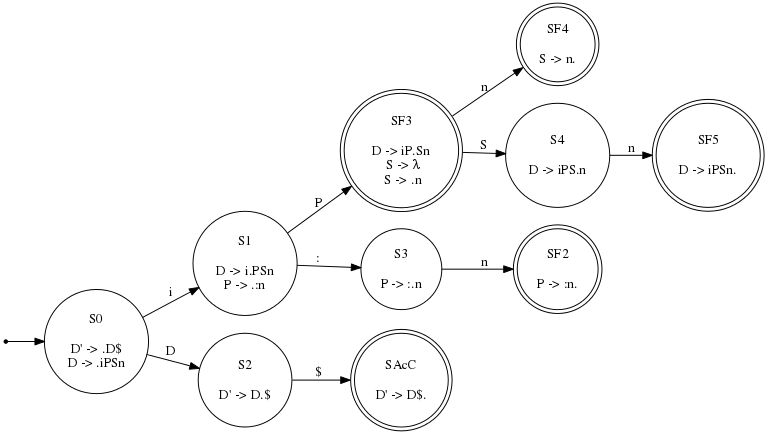
\includegraphics[scale=0.65]{tex/ejerciciosHoja3/automata_H3E4.png}
\end{center}

\ppart
\begin{tabular}{| c | c | c | c | c | c | c | c | }
\hline
Estado & i & n & : & \$ & D & P & S\\
\hline
S0 & d1 & &  &  & 2 &  & \\
\hline
S1 &  &  & d3 &  &  & F3 & \\
\hline
S2 &  &  &  & dacc &  & F5 &\\
\hline
SF3 & r3 & \textcolor{red}{r3/df4} & r3 & r3 &  &  & 4\\
\hline
S3 &  & dF2 & &  &  &  & \\
\hline
SF4 & r4  & r4  & r4 & r4 & &  &\\
\hline
S4 &  & dF5 &  &  &  &  & \\
\hline
SF2 & r2 & r2 & r2 & r2 &  &  & \\
\hline
SF5 & r1 & r1 & r1 & r1 &  &  & \\
\hline
\end{tabular}
\ppart \textbf{No se trata de una gramática LR(0)} ya que hay ocasiones en las que observamos un conflico desplazamiento-reducción. Por ejemplo, en el estado inicial podemos reducir la S o desplazar según la entrada dada.

Para ver si se trata de una gramática SLR(1) vamos a ver si somos capaces de solucionar los conflictos sabiendo cuales son los elementos siguientes:
\begin{itemize}
\item siguiente(D)={\$} : solo reducimos la regla 1 si después hay un '\$'.
\item siguiente(P)={n} : solo reducimos la regla 2 si después hay una 'n'.
\item siguiente(S)={n} : solo reducimos las reglas 3 y 4 si después hay una 'n'.
\end{itemize}

Sin embargo, \textbf{tampoco se trata de una gramática SLR(1)} ya que si forzamos a que las reducciones se produzcan en presencia del siguiente elemento no evitamos el conflicto. Como el siguiente de S es n, en presencia de esta n podremos aplicar la reducción S ::= λ o desplazar según la regla S ::= n. Quedando la siguiente tabla SLR(1):

\begin{tabular}{| c | c | c | c | c | c | c | c | }
\hline
Estado & i & n & : & \$ & D & P & S\\
\hline
S0 & d1 & &  &  & 2 &  & \\
\hline
S1 &  &  & d3 &  &  & F3 & \\
\hline
S2 &  &  &  & dacc &  & F5 &\\
\hline
SF3 &  & \textcolor{red}{r3/df4} &  &  &  &  & 4\\
\hline
S3 &  & dF2 & &  &  &  & \\
\hline
SF4 &   & r4  &  &  & &  &\\
\hline
S4 &  & dF5 &  &  &  &  & \\
\hline
SF2 &  & r2 &  &  &  &  & \\
\hline
SF5 &  &  &  & r1  &  &  & \\
\hline
\end{tabular}

\end{problem}

%%%%%%%%%%%%%%%%%%%%%%%%%%%%%%%%%%%%%%%%%%%%%%%
%%%
%%% 		Problema 5
%%%
%%%%%%%%%%%%%%%%%%%%%%%%%%%%%%%%%%%%%%%%%%%%%%%
\begin{problem}
Sea la siguiente gramática:
\begin{itemize}
\item S ::= bLd
\item L ::= E;L
\item L ::= λ
\item E ::= i=c
\item E ::= b
\end{itemize}
\ppart Dibuja el diagrama de estados del analizador LR(0) para dicha gramática
\ppart Calcula la tabla de análisis para el analizador LR(0)
\ppart Indica justificadamente si es SLR(1)

\solution
\ppart Extendemos la gramática para realizar el análisis LR(0):

\begin{itemize}
\item (0) S' ::= S \$
\item (1) S ::= bLd
\item (2) L ::= E;L
\item (3) L ::= λ
\item (4) E ::= i=c
\item (5) E ::= b
\end{itemize}
\begin{center}
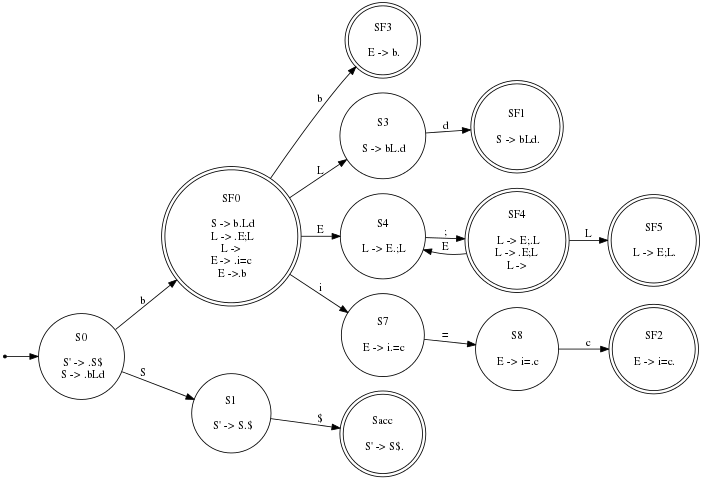
\includegraphics[scale=0.65]{tex/ejerciciosHoja3/automata5.png}
\end{center}

\ppart
\begin{tabular}{| c | c | c | c | c | c | c | c | c | c | c | }
\hline
Estado  & i & = & c & ; & b & d & \$ & L & E & S \\
\hline
S0 &  &  &  &  & dF0 &  &  &  &  & 1\\
\hline
S1 &  &  &  &  &  &  & dacc &  &  & \\
\hline
SF0 & \textcolor{red}{r3/d7} & r3 & r3 & r3 & \textcolor{red}{r3/dF3} & r3 & r3 & 3 & 4 & \\
\hline
S3 &  &  &  &  &  & dF1 &  &  &  & \\
\hline
SF1 & r1 & r1 & r1 & r1 & r1 & r1 & r1 &  &  & \\
\hline
S4 &  &  &  & dF4 &  &  &  &  &  & \\
\hline
SF4 & r3 & r3 & r3 & r3 & r3 & r3 & r3 & F5 & 4 & \\
\hline
SF5 & r2 & r2 & r2 & r2 & r2 & r2 & r2 &  &  & \\
\hline
SF3 & r5 & r5 & r5 & r5 & r5 & r5 & r5 &  &  & \\
\hline
S7 &  & d8 &  &  &  &  &  &  &  & \\
\hline
S8 &  &  & dF2 &  &  &  &  &  &  & \\
\hline
SF2 & r4 & r4 & r4 & r4 & r4 & r4 & r4 &  &  & \\
\hline
\end{tabular}
\ppart \textbf{No se trata de una gramática LR(0)} ya que hay ocasiones en las que observamos un conflicto desplazamiento-reducción.

Para ver si se trata de una gramática SLR(1) vamos a ver si somos capaces de solucionar los conflictos sabiendo cuales son los elementos siguientes:
\begin{itemize}
\item siguiente(L)={d} : solo reducimos las reglas 2 y 3 si después hay una 'd'.
\item siguiente(E)={;} : solo reducimos las reglas 4 y 5 si después hay un ';'.
\item siguiente(S)={\$} : solo reducimos la regla 1 si después hay un '\$'.
\end{itemize}

Se corrigen los dos conflictos que hay ya que en el estado SF0 solo reduciremos si llega una 'd', por tanto en el caso de que llegue una 'b' o una 'i' desplazaremos. Quedando la tabla así:

\begin{tabular}{| c | c | c | c | c | c | c | c | c | c | c | }
\hline
Estado  & i & = & c & ; & b & d & \$ & L & E & S \\
\hline
S0 &  &  &  &  & dF0 &  &  &  &  & 1\\
\hline
S1 &  &  &  &  &  &  & dacc &  &  & \\
\hline
SF0 & d7 &  &  &  & dF3 & r3 &  & 3 & 4 & \\
\hline
S3 &  &  &  &  &  & dF1 &  &  &  & \\
\hline
SF1 &  &  &  &  &  &  & r1 &  &  & \\
\hline
S4 &  &  &  & dF4 &  &  &  &  &  & \\
\hline
SF4 &  &  &  &  &  & r3 &  & F5 & 4 & \\
\hline
SF5 &  &  &  &  &  & r2 &  &  &  & \\
\hline
SF3 &  &  &  & r5 &  &  &  &  &  & \\
\hline
S7 &  & d8 &  &  &  &  &  &  &  & \\
\hline
S8 &  &  & dF2 &  &  &  &  &  &  & \\
\hline
SF2 &  &  &  & r4 &  &  &  &  &  & \\
\hline
\end{tabular}

\end{problem}

%%%%%%%%%%%%%%%%%%%%%%%%%%%%%%%%%%%%%%%%%%%%%%%
%%%
%%% 		Problema 6
%%%
%%%%%%%%%%%%%%%%%%%%%%%%%%%%%%%%%%%%%%%%%%%%%%%
\begin{problem}
Calcula los conjuntos primero y siguiente de todos los símbolos no terminales de las gramáticas siguientes

\ppart
\begin{itemize}
\item X ::= Ye
\item X ::= eYZf
\item Y ::= g
\item Y ::= Yg
\item Z ::= h
\end{itemize}

\ppart
\begin{itemize}
\item Q ::= fXY
\item X ::= cQ
\item X ::= λ
\item Y ::= iQ
\item Y ::= λ
\end{itemize}

\ppart
\begin{itemize}
\item A ::= BXB
\item X ::= ,
\item X ::= .
\item X ::= e
\item B ::= 0B
\item B ::= 1B
\item B ::= λ
\end{itemize}

\solution
\spart
\begin{itemize}
\item primero(X)=\{e,g\}
\item primero(Y)=\{g\}
\item primero(Z)=\{h\}
\end{itemize}
\begin{itemize}
\item siguiente(X)=\{\$\}
\item siguiente(Y)=\{\$,e,h\}
\item siguiente(Z)=\{\$,f\}
\end{itemize}

\newpage

\spart
\begin{itemize}
\item primero(Q)=\{f\}
\item primero(X)=\{c,λ\}
\item primero(Y)=\{i,λ\}
\end{itemize}
\begin{itemize}
\item siguiente(Q)=\{\$\} $\cup$ siguiente(X) $\cup$ siguiente(Y) = \{\$, i\}
\item siguiente(X)=\{i\} $\cup$ siguiente(Q) = \{\$, i\}
\item siguiente(Y)=siguiente(Q) = \{\$, i\}
\end{itemize}

\spart
\begin{itemize}
\item primero(X)=\{",",.,e\}
\item primero(A)=\{0,1,",",.,e\}
\item primero(B)=\{0,1,",",.,e\}
\end{itemize}
\begin{itemize}
\item siguiente(X)=\{\$,0,1\}
\item siguiente(A)=\{\$,\}
\item siguiente(B)=\{\$,",",.,e\}
\end{itemize}

\end{problem}

%%%%%%%%%%%%%%%%%%%%%%%%%%%%%%%%%%%%%%%%%%%%%%%
%%%
%%% 		Problema 7
%%%
%%%%%%%%%%%%%%%%%%%%%%%%%%%%%%%%%%%%%%%%%%%%%%%
\begin{problem}
Cacula los símbolos de adelanto para el cierre de las siguientes reglas y gramáticas:
\ppart Cierre de E' ::= .E $\{ \$ \}$ para la siguiente gramática
\begin{itemize}
\item E' ::= E
\item E ::= T
\item E ::= E+T
\item T ::= i
\item T ::= (E)
\end{itemize}

\ppart Cierre de S' ::= .s $\{ \$ \}$ para la siguiente gramática
\begin{itemize}
\item S' ::= S
\item S ::= L=R
\item S ::= R
\item L ::= *R
\item L ::= i
\item R ::= L
\end{itemize}

\ppart Cierre de E ::= (.E) $\{ \$ \}$ para la siguiente gramática
\begin{itemize}
\item E ::= (L)
\item E ::= a
\item L ::= L,E
\item L ::= E
\end{itemize}
\solution
\ppart
El cierre, con los conjuntos de adelanto, sería
\begin{itemize}
\item E' ::= .E $\{\$\}$
\item E ::= .T $\{\$\}$
\item E ::= .E+T $\{+,\$\}$
\item T ::= .i $\{+,\$\}$
\item T ::= .(E) $\{\$\}$
\end{itemize}

\ppart
\begin{itemize}
\item S' ::= .S $\{\$\}$
\item S ::= .L=R $\{\$\}$
\item S ::= .R $\{\$\}$
\item L ::= .*R $\{=, \$\}$
\item L ::= .i $\{=, \$\}$
\item R ::= .L $\{\$\}$
\end{itemize}

\ppart
\begin{itemize}
\item E ::= (.L) $\{\$\}$
\item L ::= .L,E $\{",", )\}$
\item L ::= .E $\{",", )\}$
\item E ::= .a $\{",", )\}$
\item E ::= .(L) $\{",", )\}$
\end{itemize}
\end{problem}

%%%%%%%%%%%%%%%%%%%%%%%%%%%%%%%%%%%%%%%%%%%%%%%
%%%
%%% 		Problema 8
%%%
%%%%%%%%%%%%%%%%%%%%%%%%%%%%%%%%%%%%%%%%%%%%%%%
\begin{problem}
Sea la siguiente gramática independiente del contexto:
\begin{itemize}
\item S ::= aSb
\item S ::= ab
\end{itemize}
\ppart Dibuja el diagrama de estados del analizador LR(1) para dicha gramática
\ppart Calcula la tabla de análisis para el analizador LR(1)
\ppart Usa la tabla de análisis para analizar la sentencia $aabb$
\ppart Dibuja esquemáticamente el diagrama de estados LALR(1). Es suficiente con indicar los nombres de los estados, especificando cuáles son la unión de otros en LR(1).
\solution
\ppart
\begin{center}
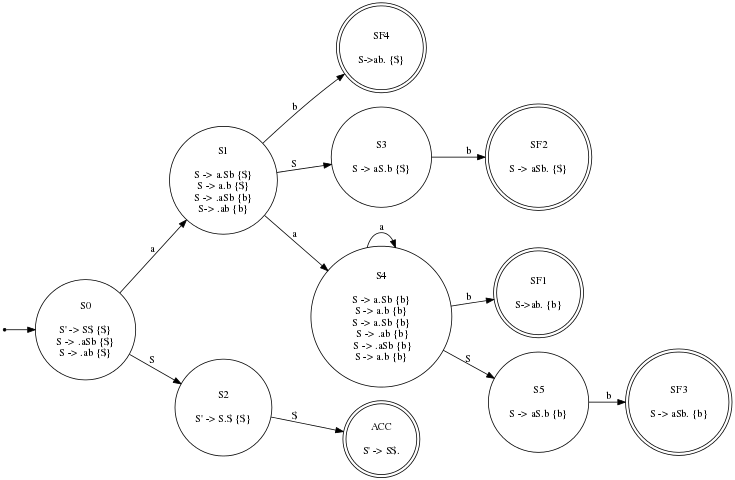
\includegraphics[scale=0.65]{tex/ejerciciosHoja3/automata_H3E8.png}
\end{center}

\ppart
\begin{tabular}{| c | c | c | c | c |}
\hline
Estado & S & a & b & \$\\
\hline
S0 & S2 & S1 & & \\
\hline
S1 & S3 & S4 & SF4 & \\
\hline
S2 & & & & ACC \\
\hline
S3 & & & SF2 & \\
\hline
S4 & S5 & S4 & SF1 & \\
\hline
S5 & & & SF3 & \\
\hline
SF1 & & & r3 & \\
\hline
SF2 & & & & r2\\
\hline
SF3 & & & r2 & \\
\hline
SF4 & & & & r3 \\
\hline
\end{tabular}

\ppart
La secuencia de acciones sería la siguiente:
\begin{verbatim}
Cadena: .aabb / Leemos 'a' y pasamos a S1
Cadena: a.abb / Leemos 'a' y pasamos a S4
Cadena: aa.bb / Leemos b y pasamos a SF1
Cadena: aab.b / Como el siguiente elemento a leer es b reducimos y volvemos a S0
Cadena: .aSb / Leemos 'a' y pasamos a S1
Cadena: a.Sb / Leemos 'S' y pasamos a S3
Cadena: aS.b / Leemos 'b' y pasamos a SF2
Cadena: aSb. / Como el siguiente elemento a leer es $, reducimos y volvemos a S0
Cadena: .S / Leemos S y pasamos a S2
Cadena: . / Fin de cadena. Llegados a este punto aceptamos la entrada
\end{verbatim}

\ppart
Cuando pasemos de LR(1) a LALR(1) vamos a agrupar los nodos SF4 y SF1 en uno solo así como SF2 y SF3, manteniendo las mismas reglas en cada caso y estableciendo como símbolos de adelanto la unión de los símbolos de adelanto de las reglas de los estados a unir.
\end{problem}

%%%%%%%%%%%%%%%%%%%%%%%%%%%%%%%%%%%%%%%%%%%%%%%
%%%
%%% 		Problema 9
%%%
%%%%%%%%%%%%%%%%%%%%%%%%%%%%%%%%%%%%%%%%%%%%%%%
\begin{problem}
Sea la siguiente gramática independiente del contexto:
\begin{itemize}
\item S ::= XX
\item X ::= aX
\item X ::= b
\end{itemize}
\ppart Dibuja el diagrama de estados del analizador LR(1) para dicha gramática
\ppart Calcula la tabla de análisis para el analizador LR(1)
\ppart Usa la tabla de análisis para analizar la sentencia $aabb$
\ppart Dibuja esquemáticamente el diagrama de estados LALR(1). Es suficiente con indicar los nombres de los estados, especificando cuáles son la unión de otros en LR(1).
\solution
\ppart Extendemos la gramática para realizar el análisis LR(1):

\begin{itemize}
\item (0) S' ::= S
\item (1) S ::= XX
\item (2) X ::= aX
\item (3) X ::= b
\end{itemize}
\begin{center}
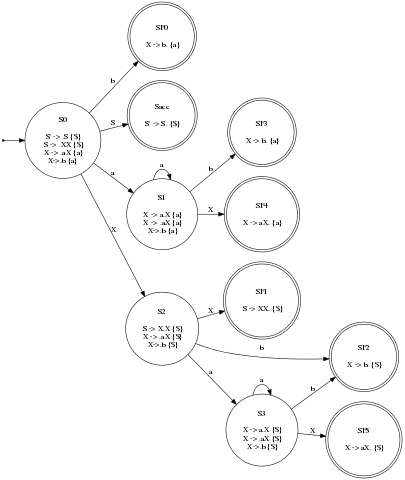
\includegraphics[scale=0.65]{tex/ejerciciosHoja3/automata9.png}
\end{center}

\ppart
\begin{tabular}{| c | c | c | c | c | }
\hline
Estado  & a & b & X & S \\
\hline
S0 & d1 & dF0 & acc & 2\\
\hline
SF0 & r3  & r3 &  & \\
\hline
S1 & d1 & dF3 & F4 &  \\
\hline
SF3 & r3 & r3 &  & \\
\hline
SF4 & r2 & r2 &  &   \\
\hline
S2 & d3 & dF2 & F1 &  \\
\hline
SF1 & r1 & r1 &  &  \\
\hline
S3 & d3 & dF2 & F5 & \\
\hline
SF5 & r2 & r2 &  &  \\
\hline
SF2 & r3 & r3 &  &  \\
\hline
\end{tabular}


\end{problem}

%%%%%%%%%%%%%%%%%%%%%%%%%%%%%%%%%%%%%%%%%%%%%%%
%%%
%%% 		Problema 10
%%%
%%%%%%%%%%%%%%%%%%%%%%%%%%%%%%%%%%%%%%%%%%%%%%%
\begin{problem}
Sea la siguiente gramática

\begin{itemize}
\item D ::= iPSn
\item P ::= :n
\item S ::= λ
\item S ::= n
\end{itemize}

\ppart Dibuja el diagrama de estados del analizador LR(1) para dicha gramática
\ppart Calcula la tabla de análisis para el analizador LR(1)
\ppart Indica justificadamente si la gramática es LR(1). Indica justificadamente si es SLR(1)
\solution
\ppart Extendemos la gramática para realizar el análisis LR(1):

\begin{itemize}
\item (0) S' ::= S
\item (1) S ::= XX
\item (2) X ::= aX
\item (3) X ::= b
\end{itemize}
\begin{center}
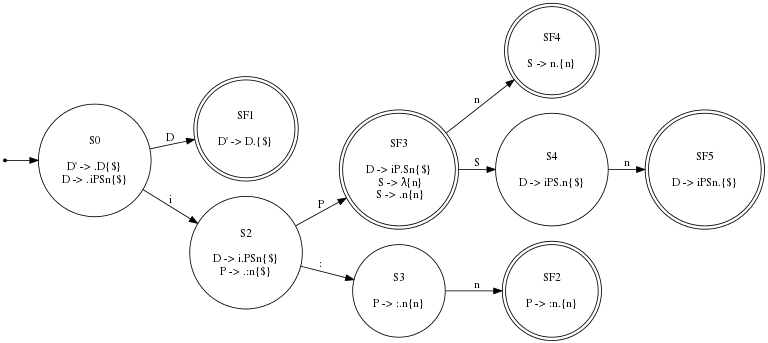
\includegraphics[scale=0.65]{tex/ejerciciosHoja3/automata10.png}
\end{center}

\ppart
\begin{tabular}{| c | c | c | c | c | c | c | c | }
\hline
Estado & i & n & : & \$ & D & P & S\\
\hline
S0 & d1 & &  &  & 2 &  & \\
\hline
S1 &  &  & d3 &  &  & F3 & \\
\hline
S2 &  &  &  & dacc &  & F5 &\\
\hline
SF3 & r3 & \textcolor{red}{r3/df4} & r3 & r3 &  &  & 4\\
\hline
S3 &  & dF2 & &  &  &  & \\
\hline
SF4 & r4  & r4  & r4 & r4 & &  &\\
\hline
S4 &  & dF5 &  &  &  &  & \\
\hline
SF2 & r2 & r2 & r2 & r2 &  &  & \\
\hline
SF5 & r1 & r1 & r1 & r1 &  &  & \\
\hline
\end{tabular}


\ppart
No es LR(1) porque sigue habiendo conflictos.
\end{problem}



\printindex
\end{document}
